\documentclass[smallabstract,smallcaptions]{dccpaper}
%
\usepackage{amssymb,amsthm}
\usepackage{thmtools}
\usepackage{amsxtra,amsfonts}
\usepackage[dvipsnames]{xcolor}
\usepackage{enumitem}
\usepackage{mathtools}
\usepackage{enumitem}
\usepackage{latexsym}
\usepackage{mathrsfs}
\newtheorem{prop}{Proposition}
\newtheorem{Def}{Definition}
\newtheorem{lemma}{Lemma}
\newtheorem{theorem}{Theorem}
\newcounter{MYtempeqncnt}
\usepackage{algorithm}
\usepackage{algorithmic}
\newcommand{\V}{\mathbf{V}}
\newcommand{\hP}{\widehat{P}}
\newcommand{\hQ}{\widehat{Q}}
\newcommand{\bX}{\mathbf{X}}
\newcommand{\bZ}{\mathbf{Z}}
\newcommand{\bR}{\mathbf{R}}
\newcommand{\bV}{\mathbf{V}}
\newcommand{\bU}{\mathbf{U}}
\newcommand{\interior}[1]{%
  {\kern0pt#1}^{\mathrm{o}}%
}
\newcommand{\disfunction}{distortion function}
  
\usepackage{verbatim}
\usepackage{srcltx}

\usepackage[utf8]{inputenc}                                         % -> damit man sie auch gleich im Code eingeben kann
\usepackage[T1]{fontenc}
\usepackage[pdfborder={0 0 0},colorlinks,citecolor=blue,hyperindex=true,hypertexnames=false,extension=pdf]{hyperref} 
\newenvironment{shrinkeq}[1]
{ \bgroup
  \addtolength\abovedisplayshortskip{#1}
  \addtolength\abovedisplayskip{#1}
  \addtolength\belowdisplayshortskip{#1}
  \addtolength\belowdisplayskip{#1}}
{\egroup\ignorespacesafterend}

\graphicspath{{../jpg/}{../pdf/}{../jpeg/}{../eps/}}
\DeclareGraphicsExtensions{.jpg,.pdf,.jpeg,.png,.eps}
\pagenumbering{plain}
%\usepackage[shortlabels]{enumitem}

% *** SUBFIGURE PACKAGES ***
\usepackage[caption=false,font=footnotesize]{subfig}
% correct bad hyphenation here
\hyphenation{op-tical net-works semi-conduc-tor}
\usepackage{setspace}

\usepackage{amsmath}
% header Datei
%%%%%%%%%%%%%%%%%%%%%%%%%%%%%%%%%%%%%%%%%%%%%%%%%%%%%%55
\usepackage{tensor} % noetig für einige indizes. Sieht sonst scheisse aus.

\usepackage{cleveref} % referenzing mulitple equations package,http://www.ctan.org/tex-archive/macros/latex/contrib/cleveref/ 
\newcommand{\crefrangeconjunction}{--}

% neues für sparseconv2 arxiv
\newcommand{\mgeq}{\succeq}

%%%%%% Hennings Abkürzungen:start

% Skalarräume
\newcommand{\NO}{\mathbb{N_0}}
\newcommand{\Ngzero}{{\mathbb{N}_{>0}}}

% Vektorräume
\newcommand{\spaceS}{{\mathcal S}}

% Funktionenräume
\newcommand{\Lp}{{L}^p}
\newcommand{\Linf}{{L}^\infty}


% indices of Dimensions, functions, etc
\newcommand{\xone}{\ensuremath{x_1}}
\newcommand{\xtwo}{\ensuremath{x_2}}

\newcommand{\hd}{\ensuremath{\hat{d}}}
\newcommand{\dzero}{\ensuremath{d_0}}
\newcommand{\done}{\ensuremath{d_1}}
\newcommand{\dtwo}{\ensuremath{d_2}}
\newcommand{\dK}{\ensuremath{d_K}}
\newcommand{\hdzero}{\ensuremath{\hd_0}}
\newcommand{\hdone}{\ensuremath{\hd_1}}
\newcommand{\hdtwo}{\ensuremath{\hd_2}}
\newcommand{\hdK}{\ensuremath{\hd_K}}

\newcommand{\Lone}{{{L}_1}}
\newcommand{\Ltwo}{{{L}_2}}
\newcommand{\tLone}{{\tilde{L}}_1}
\newcommand{\tLtwo}{{\tilde{L}}_2}

% Folgenräume
\newcommand{\lp}{{\ell^p}}
\newcommand{\linf}{{\ell^\infty}}
\newcommand{\ltwo}{{\ell^2}}
\newcommand{\lone}{{\ell^1}}

\newcommand{\begriff}[1]{\textcolor{red}{\bf #1}}

% Kürzel für oft gebrauchte Ausdrücke
\newcommand{\normtwo}[1]{\left\|#1\right\|_{\ell^2}}
\newcommand{\normp}[1]{\left\|#1\right\|_{\ell^p}}
\newcommand{\abs}[1]{\left|#1\right|}
\newcommand{\onehalf}{\frac{1}{2}}
\newcommand{\oneover}[1]{\frac{1}{#1}}
\newcommand{\twopi}{{2\pi}}
%\newcommand{\curve}{{\mathcal C}}

% Zeichen
\newcommand{\om}{\omega}
\newcommand{\Om}{\Omega}
\newcommand{\opdot}{\;\cdot\;}

% Integrale
\newcommand{\intpi}{\int_{-\pi}^\pi}
\newcommand{\intinf}{\int_{-\infty}^\infty}
\newcommand{\intones}{\int_{-1}^1}
\newcommand{\intzeroone}{\int_0^1}
\newcommand{\intzero}{\int_0}
\newcommand{\intsym}[1]{\int_{-#1}^{#1}}

\newcommand{\dt}{\mathrm dt}
\newcommand{\dw}{\mathrm d\omega}
\newcommand{\dtau}{\mathrm d\tau}
\newcommand{\dz}{\mathrm dz}
\newcommand{\dx}{\mathrm dx}

% Summen
\newcommand{\suminf}[1][k]{\sum_{#1=-\infty}^\infty}
\newcommand{\sumnN}{\sum_{n=1}^N}
\newcommand{\sumsym}[2][N]{\sum_{#1=-#2}^{#2}}

% Folgen
\newcommand{\seq}[1]{\left\{#1\right\}}
\newcommand{\seqkZ}[1]{\seq{#1}_{k\in\Z}}
\newcommand{\seqnZ}[1]{\seq{#1}_{n\in\Z}}
\newcommand{\seqkN}[1]{\seq{#1}_{k\in\N}}
\newcommand{\seqnN}[1]{\seq{#1}_{n\in\N}}

% Sinc
\newcommand{\sincfrac}[1][t]{\frac{\sin(\pi #1)}{\pi #1}}
\newcommand{\sincfracz}{\frac{\sin(\pi z)}{\pi z}}
\newcommand{\sinc}{\ensuremath{\operatorname{sinc}}}
\newcommand{\versine}{\ensuremath{\operatorname{versine}}}

% Weitere Operatoren
\newcommand{\dist}{\operatorname{dist}}
%\renewcommand{\span}[1]{{\operatorname{span}\left\{#1\right\}}}
\newcommand{\scp}[1]{\left\langle #1 \right\rangle}
\newcommand{\dual}[1]{{#1}^\ast}
\newcommand{\bidual}[1]{{#1}^{\ast\ast}}
\newcommand{\inn}{\operatorname{int}}
%%%%%%%%%\newcommand{\graph}{\operatorname{graph}}
\newcommand{\gdw}{\Leftrightarrow}
\newcommand{\grad}{\triangledown}
\newcommand{\codim}{\operatorname{codim}}
\renewcommand{\P}{\operatorname{Pr}}
\newcommand{\diag}{\operatorname{diag}}
\newcommand{\sgn}{\operatorname{sgn}}
\newcommand{\modulo}{\operatorname{mod}}

\newcommand{\otriangle}{\circledcirc} % in MnSymbol package defined as circled triangle

% Schwache Konvergenz
\newcommand{\wto}{\rightharpoonup}
\newcommand{\wsto}{\overset{\ast}\rightharpoonup}

% For all
\let\forallalt\forall
\renewcommand{\forall}{\;\forallalt\;}

% Ref mit Klammern
\let\refalt\ref
\renewcommand{\ref}[1]{(\refalt{#1})}

% IEEE
\renewcommand{\vec}{\mathbf}

%%%%%% Hennings Abkürzungen:ende


%---------------%
% Abbreviations %
%---------------%

% kleine griechische = Winkel, große = Mengen 
\newcommand{\alp}{\ensuremath{\alpha}}
\newcommand{\bet}{\ensuremath{\beta}}
\newcommand{\Del}{\ensuremath{\Delta}}
\newcommand{\del}{\ensuremath{\delta}}
\newcommand{\eps}{\ensuremath{\epsilon}}
\newcommand{\Gam}{\ensuremath{\Gamma}}
\newcommand{\gam}{\ensuremath{\gamma}}
\newcommand{\Lam}{\ensuremath{\Lambda}}
\newcommand{\lam}{\ensuremath{\lambda}}
\newcommand{\kap}{\ensuremath{\kappa}}
\newcommand{\Ome}{\ensuremath{\Omega}}
\newcommand{\ome}{\ensuremath{\omega}}
\newcommand{\Sig}{\ensuremath{\Sigma}}
\newcommand{\sig}{\ensuremath{\sigma}}
\newcommand{\tht}{\ensuremath{\theta}}
\newcommand{\zet}{\ensuremath{\zeta}}

\newcommand{\zetkl}{\ensuremath{\zeta_{k_l}}}


\newcommand{\phii}{{ \ensuremath{ \phi_i} }}
\newcommand{\tphi}{{ \ensuremath{ \tilde{\phi}} }}
\newcommand{\tome}{{ \ensuremath{ \tilde{\ome}} }}
\newcommand{\tzeta}{{ \ensuremath{ \tilde{\zeta}} }}
\newcommand{\tvphi}{{ \ensuremath{ \tilde{\vphi}} }}
\newcommand{\ttht}{{ \ensuremath{ \tilde{\tht}} }}
\newcommand{\tPhi}{{ \ensuremath{ \tilde{\Phi}} }}
\newcommand{\phik}{{ \ensuremath{ \phi_k} }}
\newcommand{\phij}{{ \ensuremath{ \phi_j} }}
\newcommand{\phijp}{{ \ensuremath{ {\phi'}_j} }}
\newcommand{\eip}[1]{\ensuremath{e^{i2\pi #1}} }
\newcommand{\alpj}{\ensuremath{\alp_j}}
\newcommand{\betj}{\ensuremath{\bet_j}}

% vectoren (v) mit normal (), tilde (t), prime (p)
% Vektoren werden klein und fett geschrieben, Vektoroperatoren werden gro{\ss} und fett geschrieben


\newcommand{\vOme}{\ensuremath{\mathbf{\Omega}}}
\newcommand{\vGam}{\ensuremath{\mathbf{\Gam}}}
\newcommand{\vGamnull}{\ensuremath{\mathbf{R}}}     % von Henning übernommen, reversal matrix
\newcommand{\vGamnulln}{\ensuremath{\mathbf{R}}_{n}}
\newcommand{\vGamnullN}{\ensuremath{\mathbf{R}}_{N}}
\newcommand{\vgam}{\ensuremath{\boldsymbol{ \gam}}}
\newcommand{\vLam}{\ensuremath{\mathbf{\Lambda}}}
\newcommand{\vlam}{\ensuremath{\boldsymbol{ \lam}}}
\newcommand{\vtlam}{\ensuremath{\tilde{\boldsymbol{ \lam}}}}
\newcommand{\hvlam}{\ensuremath{\hat{\boldsymbol{ \lam}}}}

\newcommand{\vphi}{\ensuremath{\boldsymbol{ \phi}}}
\newcommand{\vpsi}{\ensuremath{\boldsymbol{ \psi}}}
\newcommand{\vtau}{\ensuremath{\boldsymbol \tau }}                         % Vektorwertige Funktion

\newcommand{\vm}{\ensuremath{\mathbf m}}
\newcommand{\vdel}{\ensuremath{\boldsymbol \delta}}
\newcommand{\veka}{\ensuremath{\mathbf a}}
\newcommand{\vnu}{\ensuremath{\boldsymbol \nu}}
\newcommand{\vmu}{\ensuremath{\boldsymbol \mu}}

% Vektoren (v)
\newcommand{\va}{{\ensuremath{\mathbf a}}}
\newcommand{\vb}{{\ensuremath{\mathbf b}}}
\newcommand{\vc}{{\ensuremath{\mathbf c}}}
\newcommand{\vd}{{\ensuremath{\mathbf d}}}
%\newcommand{\ve}{{\ensuremath{\mathbf{4}}}} % old version -> used for noise now
\newcommand{\ve}{{\ensuremath{\boldsymbol{\del}}}} % better and new version
\newcommand{\verr}{{\ensuremath{\boldsymbol{e}}}} % better and new version
\newcommand{\vf}{{\ensuremath{\mathbf f}}}
\newcommand{\vg}{{\ensuremath{\mathbf g}}}
\newcommand{\vh}{{\ensuremath{\mathbf h}}}                         % Vektorwertige Funktion
\newcommand{\vn}{{\ensuremath{\mathbf n}}}                         % Vektorwertige Funktion
\newcommand{\vp}{{\ensuremath{\mathbf p}}}
\newcommand{\vq}{{\ensuremath{\mathbf q}}}
\newcommand{\vqx}{{\ensuremath{\mathbf q}}}
\newcommand{\vqy}{{\ensuremath{\mathbf p}}}
\newcommand{\vr}{{\ensuremath{\mathbf r}}}                         % Vektorwertige Funktion
\newcommand{\vs}{{\ensuremath{\mathbf s}}}
\newcommand{\vt}{{\ensuremath{\mathbf t}}}
\newcommand{\vu}{{\ensuremath{\mathbf u}}}
\newcommand{\vv}{{\ensuremath{\mathbf v}}}
\newcommand{\vw}{{\ensuremath{\mathbf w}}}
\newcommand{\vx}{{\ensuremath{\mathbf x}}}
\newcommand{\vy}{{\ensuremath{\mathbf y}}}



\newcommand{\vue}{{\ensuremath{\mathbf u}_1}}
\newcommand{\vuz}{{\ensuremath{\mathbf u}_2}}
\newcommand{\vxe}{{\ensuremath{\mathbf x}_1}}
\newcommand{\vxz}{{\ensuremath{\mathbf x}_2}}
\newcommand{\vtxe}{{\ensuremath{\tilde{\mathbf x}}_1}}
\newcommand{\vtxz}{{\ensuremath{\tilde{\mathbf x}}_2}}
\newcommand{\vye}{{\ensuremath{\mathbf y}_1}}
\newcommand{\vyz}{{\ensuremath{\mathbf y}_2}}
\newcommand{\vxone}{{\ensuremath{\mathbf x}_1}}
\newcommand{\vxtwo}{{\ensuremath{\mathbf x}_2}}
\newcommand{\tvxone}{{\ensuremath{\tilde{\mathbf x}_1}}}
\newcommand{\tvxtwo}{{\ensuremath{\tilde{\mathbf x}_2}}}
\newcommand{\vtxone}{{\ensuremath{\tilde{\mathbf x}_1}}}
\newcommand{\vtxtwo}{{\ensuremath{\tilde{\mathbf x}_2}}}
\newcommand{\vxn}{{\ensuremath{\mathbf{ x}^n}}}
\newcommand{\vxN}{{\ensuremath{\mathbf{x}^{\Lone}_1}}}
\newcommand{\vxL}{{\ensuremath{\mathbf{x}^{\Ltwo}_2}}}
\newcommand{\vxrev}{{\ensuremath{\mathbf{ x}^-}}}
\newcommand{\vyrev}{{\ensuremath{\mathbf{ y}^-}}}
\newcommand{\vzrev}{{\ensuremath{\mathbf{ z}^-}}}
\newcommand{\vxo}{{\ensuremath{\mathbf x}^{\circ}}}
\newcommand{\vxom}{{\ensuremath{\mathbf x}^{\circ}_{-}}}
\newcommand{\vyn}{\ensuremath{ {\mathbf y}(n)} }
\newcommand{\vyL}{\ensuremath{ {\mathbf y}^{\Ltwo}} }
\newcommand{\vyN}{\ensuremath{ {\mathbf y}^{\Lone}} }
\newcommand{\vyest}{\ensuremath{{\mathbf y}^{\#}}}
\newcommand{\vz}{{\ensuremath{\mathbf z}}}

% Time-Reverse (reciprocal) vectors
\newcommand{\Rx}{{\ensuremath{x}^{-}}}
\newcommand{\Ry}{{\ensuremath{y}^{-}}}
\newcommand{\Rtx}{{\ensuremath{\tx}^{-}}}
\newcommand{\Rty}{{\ensuremath{\ty}^{-}}}
\newcommand{\Rvx}{{\ensuremath{\mathbf x}^{-}}}
\newcommand{\Rvxj}{{\ensuremath{\mathbf x}^{-}_j}}
\newcommand{\Rxone}{\ensuremath{ x_1^{-}}}
\newcommand{\Rxtwo}{\ensuremath{ x_2^{-}}}
\newcommand{\Rvxone}{\ensuremath{{\mathbf x}_1^{-}}}
\newcommand{\Rvxtwo}{{\ensuremath{\mathbf x}_2^{-}}}

% sepcial vectors
\newcommand{\vpilot}{\ensuremath{\vp}}

% vector (v) mit tilde (t)
\newcommand{\vta}{\ensuremath{\tilde{\mathbf a}}}
\newcommand{\vtb}{\ensuremath{\tilde{\mathbf b}}}
\newcommand{\vtd}{\ensuremath{\tilde{\mathbf d}}}
\newcommand{\vtg}{\ensuremath{\tilde{\mathbf g}}}
\newcommand{\vth}{\ensuremath{\tilde{\mathbf h}}}
\newcommand{\vtu}{\ensuremath{\tilde{\mathbf u}}}
\newcommand{\vtq}{\ensuremath{\tilde{\mathbf q}}}
\newcommand{\vtn}{\ensuremath{\tilde{\mathbf n}}}
\newcommand{\vtx}{\ensuremath{\tilde{\mathbf x}}}
\newcommand{\vttx}{\ensuremath{\tilde{\tilde{\mathbf x}}}}
\newcommand{\vtxn}{\ensuremath{\tilde{\mathbf x}^n}}
\newcommand{\vty}{\ensuremath{\tilde{\mathbf y}}}
\newcommand{\vtyn}{\ensuremath{\tilde{\mathbf y}^n}}
\newcommand{\vtz}{\ensuremath{\tilde{\mathbf z}}}

\newcommand{\vsx}{\ensuremath{{\mathbf x}^{\prime}}}
\newcommand{\vsy}{\ensuremath{{\mathbf y}^{\prime}}}

\newcommand{\vgt}{{\ensuremath{\mathbf \tilde{g}}^L}}


\newcommand{\vhi}{\ensuremath{\mathbf h^{(i)} }}                         % Vektorwertige Funktion

% vecotr (v) mit tilde (t) und prime (p)
\newcommand{\vhp}{\ensuremath{\mathbf h^{'}}}                         % Vektorwertige Funktion

\newcommand{\vgtDg}{{\ensuremath{{{\tilde{\mathbf g}}}_{\Delta,{\vg}}}}}
\newcommand{\hvgtDg}{{\ensuremath{{\hat{\tilde{\mathbf g}}}_{\Delta,{\vg}}}}}
\newcommand{\vgtDzweig}{{\ensuremath{{\tilde{\mathbf g}}_{2,{\vg}}}}}
\newcommand{\hvgtDzweig}{{\ensuremath{{\hat{\tilde{\mathbf g}}}_{2,{\vg}}}}}
\newcommand{\ihve}{{\ensuremath{\check{\ve}}}}

% sonstiges
\newcommand{\yest}{\ensuremath{{y}^{\#}}}
\newcommand{\Eps}{\ensuremath{\mathcal{E}}}

% hat(h)-vector(v)
\newcommand{\hva}{{\ensuremath{\hat{\mathbf a}}}}
\newcommand{\hvb}{{\ensuremath{\hat{\mathbf b}}}}
\newcommand{\hvc}{\ensuremath{\hat{\vc}}}
\newcommand{\hve}{{\ensuremath{\hat{\ve}}}}
\newcommand{\hvg}{{\ensuremath{\hat{\mathbf g}}}}
\newcommand{\hvh}{{\ensuremath{\hat{\mathbf h}}}}
\newcommand{\hvn}{\ensuremath{\hat{\vn}}}
\newcommand{\hvm}{\ensuremath{\hat{\vm}}}
\newcommand{\hvp}{{\ensuremath{\hat{\mathbf p}}}}
\newcommand{\hvr}{{\ensuremath{\hat{\mathbf r}}}}
\newcommand{\hvs}{{\ensuremath{\hat{\mathbf s}}}}
\newcommand{\hvu}{\ensuremath{\hat{\vu}}}
\newcommand{\hvw}{\ensuremath{\hat{\vw}}}
\newcommand{\hvx}{{\ensuremath{\hat{\mathbf x}}}}
\newcommand{\hvy}{{\ensuremath{\hat{\mathbf y}}}}
\newcommand{\hvz}{{\ensuremath{\hat{\mathbf z}}}}
\newcommand{\hvgL}{{\ensuremath{\hat{\mathbf g}}}}

% hat (h) -tilde (t) -vector (v)
\newcommand{\htvh}{{\ensuremath{\hat{\tilde{\mathbf h}}}}}
\newcommand{\htvx}{{\ensuremath{\hat{\tilde{\mathbf x}}}}}
\newcommand{\htvy}{{\ensuremath{\hat{\tilde{\mathbf y}}}}}
\newcommand{\htvz}{{\ensuremath{\hat{\tilde{\mathbf z}}}}}

\newcommand{\hvtx}{{\ensuremath{\hat{\tilde{\mathbf x}}}}}
\newcommand{\hvty}{{\ensuremath{\hat{\tilde{\mathbf y}}}}}
% Random Variables

\newcommand{\rX}{{\ensuremath{\mathrm X}}}
\newcommand{\rY}{{\ensuremath{\mathrm Y}}}

% Polynomials
\newcommand{\uA}{{\ensuremath{\mathrm A}}}
\newcommand{\uB}{{\ensuremath{\mathrm B}}}
\newcommand{\utB}{{\ensuremath{\mathrm \tilde{B}}}}
\newcommand{\uC}{{\ensuremath{\mathrm C}}}
\newcommand{\uD}{{\ensuremath{\mathrm D}}}
\newcommand{\uI}{{\ensuremath{\mathrm I}}}
\newcommand{\uX}{{\ensuremath{\mathrm X}}}
\newcommand{\uY}{{\ensuremath{\mathrm Y}}}
\newcommand{\ua}{{\ensuremath{\mathrm a}}}
\newcommand{\ub}{{\ensuremath{\mathrm b}}}
\newcommand{\utb}{{\ensuremath{\tilde{\mathrm b}}}}
\newcommand{\uc}{{\ensuremath{\mathrm c}}}
\newcommand{\ud}{{\ensuremath{\mathrm d}}}
\newcommand{\ux}{{\ensuremath{\mathrm x}}}
\newcommand{\uq}{{\ensuremath{\mathrm q}}}
\newcommand{\us}{{\ensuremath{\mathrm s}}}
\newcommand{\ur}{{\ensuremath{\mathrm r}}}
\newcommand{\upoly}{{\ensuremath{\mathrm p}}}
\newcommand{\upz}{{\ensuremath{{\mathrm p}(z)}}}
\newcommand{\uy}{{\ensuremath{\mathrm y}}}
\newcommand{\uXone}{{\ensuremath{\mathrm X}_1}}
\newcommand{\uXtwo}{{\ensuremath{\mathrm X}_2}}
\newcommand{\tuX}{{\ensuremath{\tilde{\mathrm X}}}}
\newcommand{\utY}{{\ensuremath{\tilde{\mathrm Y}}}}
\newcommand{\uZ}{{\ensuremath{\mathrm Z}}}
\newcommand{\uR}{{\ensuremath{\mathrm R}}}
\newcommand{\uH}{{\ensuremath{\mathrm H}}}
\newcommand{\uS}{{\ensuremath{\mathrm S}}}
\newcommand{\uG}{{\ensuremath{\mathrm G}}}
\newcommand{\tuG}{{\ensuremath{\tilde{\mathrm G}}}}
\newcommand{\tuI}{{\ensuremath{\tilde{\mathrm I}}}}
\newcommand{\tuR}{{\ensuremath{\tilde{\mathrm R}}}}
\newcommand{\tuS}{{\ensuremath{\tilde{\mathrm S}}}}
\newcommand{\uN}{{\ensuremath{\mathrm N}}}
\newcommand{\uT}{{\ensuremath{\mathrm T}}}
\newcommand{\uU}{{\ensuremath{\mathrm U}}}
\newcommand{\uP}{{\ensuremath{\mathrm P}}}
\newcommand{\uQ}{{\ensuremath{\mathrm Q}}}

% Matrizen
\newcommand{\vA}{{\ensuremath{\mathbf A}}}
\newcommand{\vB}{{\ensuremath{\mathbf B}}}
\newcommand{\vC}{{\ensuremath{\mathbf C}}}
\newcommand{\vD}{{\ensuremath{\mathbf D}}}
\newcommand{\vE}{{\ensuremath{\mathbf E}}}
\newcommand{\vF}{{\ensuremath{\mathbf F}}}
\newcommand{\vG}{{\ensuremath{\mathbf G}}}
\newcommand{\vH}{\ensuremath{\mathbf H }}                         % Vektorwertige Funktion
\newcommand{\vI}{\ensuremath{\mathbf H }}                         % Vektorwertige Funktion
\newcommand{\vJ}{\ensuremath{\mathbf{J}}}
\newcommand{\vL}{{\ensuremath{\mathbf L}}}
\newcommand{\vM}{\ensuremath{\mathbf M}}
\newcommand{\vP}{\ensuremath{\mathbf P }}                         % Vektorwertiges Ma{\ss}
\newcommand{\vQ}{\ensuremath{\mathbf Q}}
\newcommand{\vR}{\ensuremath{\mathbf R}}
\newcommand{\vS}{\ensuremath{\mathbf S }}                         % Vektorwertiges Ma{\ss}
\newcommand{\vT}{\ensuremath{\mathbf T}}
\newcommand{\vU}{{\ensuremath{\mathbf U}}}
\newcommand{\vV}{{\ensuremath{\mathbf V}}}
\newcommand{\vW}{{\ensuremath{\mathbf W}}}
\newcommand{\vX}{{\ensuremath{\mathbf X}}}
\newcommand{\vY}{{\ensuremath{\mathbf Y}}}
\newcommand{\vZ}{{\ensuremath{\mathbf Z}}}

% tilde (t) Matrizen
\newcommand{\vtA}{{\ensuremath{\tilde{\mathbf A}}}}
\newcommand{\vtC}{{\ensuremath{\tilde{\mathbf C}}}}
\newcommand{\vtG}{{\ensuremath{\tilde{\mathbf G}}}}
\newcommand{\vtU}{{\ensuremath{\tilde{\mathbf U}}}}
\newcommand{\vtT}{\ensuremath{\tilde{\mathbf T}}}
\newcommand{\vtX}{\ensuremath{\tilde{\mathbf X}}}

\newcommand{\vnull}{\ensuremath{\mathbf 0}}
\newcommand{\vTT}{\ensuremath{\tilde{\mathbf T} }}

% vector (v) greek letters
\newcommand{\valp}{\ensuremath{\boldsymbol{ \alp}}}
\newcommand{\vbet}{\ensuremath{\boldsymbol{ \bet}}}
\newcommand{\veps}{\ensuremath{\boldsymbol{ \eps}}} 
\newcommand{\vzet}{\ensuremath{\boldsymbol{ \zet}}}
%\newcommand{\hvbet}{\ensuremath{\hat{\boldsymbol{ \bet}}}}
\newcommand{\vome}{\ensuremath{\boldsymbol{ \ome}}}
%\newcommand{\vzet}{\ensuremath{\boldsymbol{ \zet}}}


\newcommand{\vXgt}{\ensuremath{\vX_0}} % ground truth


\newcommand{\vgm}{\ensuremath{{\mathbf g}^L_m}}
\newcommand{\zero}{{\ensuremath{\mathbf 0}}}
\newcommand{\zerom}{{\ensuremath{\mathbb 0}}}
\newcommand{\vzero}{{\ensuremath{\mathbf O}}}

\newcommand{\hvbet}{\ensuremath{\hat{\boldsymbol{ \bet}}}}
% tilde (t) vector (v) greek letters
\newcommand{\Tvalp}{\ensuremath{\tilde{\valp} }}
\newcommand{\Tvbet}{\ensuremath{\tilde{\vbet} }}
\newcommand{\Talpj}{\ensuremath{\tilde{\alpj} }}
\newcommand{\Tvphi}{\ensuremath{\tilde{\vphi} }}
\newcommand{\Tbetj}{\ensuremath{\tilde{\betj} }}
\newcommand{\Tvome}{\ensuremath{\tilde{\vome} }}
\newcommand{\xbarj}{\ensuremath{\bar{x}_j }}

\newcommand{\vPM}{\ensuremath{\mathbf P\!}_M}                         % Vektorwertiges Ma{\ss}
\newcommand{\Shift}{\ensuremath{\mathbf T }}                         % Vektorwertiges Ma{\ss}
\newcommand{\cvektor}{\ensuremath{\mathbf c }}                         % Vektorwertige Funktion



% tilde (t) versionen
\newcommand{\ta}{\ensuremath{\tilde{a}}}
\newcommand{\tb}{\ensuremath{\tilde{b}}}
\newcommand{\tc}{\ensuremath{\tilde{c}}}
\newcommand{\td}{\ensuremath{\tilde{d}}}
\newcommand{\te}{\ensuremath{\tilde{e}}}
\newcommand{\tg}{\ensuremath{\tilde{g}}}
\newcommand{\tilh}{\ensuremath{\tilde{h}}} %\tg ist schon definiert
\newcommand{\tl}{\ensuremath{\tilde{l}}}
\newcommand{\ti}{\ensuremath{\tilde{i}}}
\newcommand{\tj}{\ensuremath{\tilde{j}}}
\newcommand{\tm}{\ensuremath{\tilde{m}}}
\newcommand{\tilder}{\ensuremath{\tilde{r}}}
\newcommand{\tilr}{\ensuremath{\tilde{r}}}
\newcommand{\tn}{\ensuremath{\tilde{n}}}
\newcommand{\tp}{\ensuremath{\tilde{p}}}
\newcommand{\tq}{\ensuremath{\tilde{q}}}
\newcommand{\ts}{\ensuremath{\tilde{s}}}
\newcommand{\tilt}{\ensuremath{\tilde{t}}} % \tt ist schon belegt 
\newcommand{\tu}{\ensuremath{\tilde{u}}}
\newcommand{\tv}{\ensuremath{\tilde{v}}}
\newcommand{\tx}{\ensuremath{\tilde{x}}}
\newcommand{\ty}{\ensuremath{\tilde{y}}}
\newcommand{\tz}{\ensuremath{\tilde{z}}}

\newcommand{\iot}{\ensuremath{\iota}} %imaginaere einheit, nicht oft genutzt
\newcommand{\ted}[1]{\tensor{\delta}{#1}}
\newcommand{\tep}[1]{\tensor{\psi}{#1}}
\newcommand{\teO}[1]{\tensor{\Ome}{#1}}
\newcommand{\tee}[1]{\tensor{\eps}{#1}}
\newcommand{\thh}{\ensuremath{\tilde{h}}}

% tilde (t) sets and integers
\newcommand{\tA}{\ensuremath{\tilde{A}}}                         
\newcommand{\tB}{\ensuremath{\tilde{B}}}                         
\newcommand{\tC}{\ensuremath{\tilde{C}}}                         
\newcommand{\tF}{\ensuremath{\tilde{F}}}
\newcommand{\tH}{\ensuremath{\tilde{H}}}
\newcommand{\tI}{\ensuremath{\tilde{I}}}
\newcommand{\tJ}{\ensuremath{\tilde{J}}}
\newcommand{\tK}{\ensuremath{\tilde{K}}}
\newcommand{\tL}{\ensuremath{\tilde{L}}}
\newcommand{\tM}{\ensuremath{\tilde{M}}}
\newcommand{\tN}{\ensuremath{\tilde{N}}}
\newcommand{\tP}{\ensuremath{\tilde{P}}}
\newcommand{\tQ}{\ensuremath{\tilde{Q}}}                         
\newcommand{\tR}{\ensuremath{\tilde{R}}} % ring extension 
\newcommand{\tS}{\ensuremath{\tilde{S}}}
\newcommand{\tU}{\ensuremath{\tilde{U}}}
\newcommand{\tV}{\ensuremath{\tilde{V}}}
\newcommand{\tX}{\ensuremath{\tilde{X}}}


\newcommand{\Pn}{\ensuremath{P^{(n)}}}

% tilde (t) greek
\newcommand{\talp}{\ensuremath{\tilde{\alp}}}
\newcommand{\tbet}{\ensuremath{\tilde{\bet}}}
\newcommand{\tdel}{\ensuremath{\tilde{\del}}}
\newcommand{\tlam}{{\ensuremath{\tilde{\lam}}}}
\newcommand{\tlaminv}{{\ensuremath{\frac{1}{\sqrt{\tilde{\lam}^{M}}}}}}
\newcommand{\tmu}{{\ensuremath{\tilde{\mu}}}}
\newcommand{\ttau}{\ensuremath{\tilde\tau }}                         % Vektorwertige Funktion


\newcommand{\teps}{\ensuremath{\tilde{\eps} }}
\newcommand{\Tbet}{\ensuremath{\tilde{\bet} }}
\newcommand{\Tome}{\ensuremath{\tilde{\ome}}}

\newcommand{\vpx}{\ensuremath{\mathbf p}^X}
\newcommand{\vpy}{\ensuremath{\mathbf p}^Y}

% vector-prime versionen
\newcommand{\vsz}{\ensuremath{{\mathbf z}^{\prime}}}

% hat versionen
\newcommand{\ha}{\ensuremath{\hat{a}}}
\newcommand{\hg}{\ensuremath{\hat{g}}}
\newcommand{\hh}{\ensuremath{\hat{h}}}
\newcommand{\hn}{\ensuremath{\hat{n}}}
\newcommand{\hp}{\ensuremath{\hat{p}}}
\newcommand{\hq}{\ensuremath{\hat{q}}}
\newcommand{\hs}{\ensuremath{\hat{s}}}
\newcommand{\hu}{\ensuremath{\hat{u}}}
\newcommand{\hv}{\ensuremath{\hat{v}}}
\newcommand{\hx}{\ensuremath{\hat{x}}}
\newcommand{\hy}{\ensuremath{\hat{y}}}
\newcommand{\hz}{\ensuremath{\hat{z}}}

% hat matrix version
\newcommand{\hvA}{\ensuremath{\hat{\vA}}}
\newcommand{\hvR}{\ensuremath{\hat{\vG}}}
\newcommand{\hvH}{\ensuremath{\hat{\vH}}}
\newcommand{\hvN}{\ensuremath{\hat{\vN}}}
\newcommand{\hvP}{\ensuremath{\hat{\vP}}}
\newcommand{\hvQ}{\ensuremath{\hat{\vQ}}}
\newcommand{\hvS}{\ensuremath{\hat{\vS}}}
\newcommand{\hvU}{\ensuremath{\hat{\vU}}}
\newcommand{\hvV}{\ensuremath{\hat{\vV}}}
\newcommand{\hvX}{\ensuremath{\hat{\vX}}}
\newcommand{\hvY}{\ensuremath{\hat{\vY}}}
\newcommand{\hvZ}{\ensuremath{\hat{\vZ}}}

\newcommand{\ihx}{\ensuremath{\check{x}}}
% hat version (greek)
\newcommand{\hbet}{\ensuremath{\hat{\bet}}}
\newcommand{\hlam}{\ensuremath{\hat{\lam}}}

\newcommand{\hpo}{\ensuremath{\hat{p}^\circ}}
\newcommand{\hpoD}{\ensuremath{\hat{p}^{\Delta,\circ}}}
\newcommand{\hqo}{\ensuremath{\hat{q}^\circ}}
\newcommand{\hqoD}{\ensuremath{\hat{q}^{\Delta,\circ}}}
\newcommand{\hgo}{\ensuremath{\hat{g}^\circ}}

% hat-tilde version
\newcommand{\htx}{\ensuremath{\hat{\tx}}}
\newcommand{\hty}{\ensuremath{\hat{\ty}}}
\newcommand{\htz}{\ensuremath{\hat{\tz}}}

% hat-tilde matrix vesion
\newcommand{\htX}{\ensuremath{\hat{\tx}}}

% sets of sets
\newcommand{\Alge}{\ensuremath{\mathscr A}}
\newcommand{\Bore}{\ensuremath{\mathscr B}}
\newcommand{\Calg}{\ensuremath{\mathscr C}}
\newcommand{\Code}{\Calg}
\newcommand{\Edge}{\ensuremath{\mathscr E}}
\newcommand{\Ealg}{\ensuremath{\mathscr E}}
\newcommand{\Falg}{\ensuremath{\mathscr F}}\newcommand{\algF}{\Falg}
\newcommand{\Grap}{\ensuremath{\mathscr G}}
\newcommand{\Halg}{\ensuremath{\mathscr H}}
\newcommand{\Jalg}{\ensuremath{\mathscr J}}
\newcommand{\Salg}{\ensuremath{\mathscr S}}
\newcommand{\Vset}{\ensuremath{\mathscr V}}
\newcommand{\Walg}{\ensuremath{\mathscr W}}
\newcommand{\Pset}{\ensuremath{\mathscr P}}
\newcommand{\Sset}{\ensuremath{\mathscr S}}
\newcommand{\Ttop}{\ensuremath{\mathscr T}}
\newcommand{\Xset}{\ensuremath{\mathscr X}}  % Probabilty space
\newcommand{\Zalg}{\ensuremath{\mathscr Z}}  % Zero codebook

% Non linear maps or sets
\newcommand{\Afrak}{\ensuremath{\mathfrak A}}
\newcommand{\Bfrak}{\ensuremath{\mathfrak B}}
\newcommand{\Cfrak}{\ensuremath{\mathfrak C}}
\newcommand{\Mfrak}{\ensuremath{\mathfrak M}}
\newcommand{\Kfrak}{\ensuremath{\mathfrak K}}


\newcommand{\Nset}{{\ensuremath{\mathcal{N}}}}
\newcommand{\Aset}{{\ensuremath{\mathcal{A}}}}
\newcommand{\Zset}{{\ensuremath{\mathcal{Z}}}}
\newcommand{\Pseta}{{\ensuremath{\mathcal{P}_A}}}

\newcommand{\LAcorr}{\ensuremath{{\mathfrak A}_{\triangle}}}
\newcommand{\LAconv}{\ensuremath{{\mathfrak A}_{*}}}
\newcommand{\CAcorr}{\ensuremath{{\mathfrak A}_{\otriangle}}}
\newcommand{\tCAcorr}{\ensuremath{{\tilde{\mathfrak A}}_{\otriangle}}}
\newcommand{\CAcorrN}{\ensuremath{{\mathfrak A}^N_{\otriangle}}}
\newcommand{\CAconv}{\ensuremath{{\mathfrak A}_{\circledast}}}
\newcommand{\tCAconv}{\ensuremath{\tilde{{\mathfrak A}}_{\circledast}}}
\newcommand{\Ambi}{{\operatorname{Ag}}}

\newcommand{\Omi}{\ensuremath{\mathcal{O}}}
\newcommand{\Lamp}{\ensuremath{\Lambda_+}}
\newcommand{\Lampeins}{\ensuremath{\Lambda^{+}_{1}}}
\newcommand{\omek}{\ensuremath{\omega_k}}
\newcommand{\omeNull}{\ensuremath{\omega_{0}}}
\newcommand{\omenull}{\ensuremath{\omega_{0}}}
\newcommand{\Tomenull}{\ensuremath{\tilde{\omega}_{0}}}
\newcommand{\omeup}{\ensuremath{\omega_{\uparrow}}}
\newcommand{\omedown}{\ensuremath{\omega_{\downarrow}}}
\newcommand{\Omepeins}{\ensuremath{\Omega^{1}_+}}
\newcommand{\Omep}{\ensuremath{\Omega_{+}}}
\newcommand{\OcL}{\ensuremath{X_k\circledast Y_l}}
\newcommand{\Tcc}{\ensuremath{\circledast}}
\newcommand{\OpcLp}{\ensuremath{\Omep\circledast\Lamp}}
\newcommand{\OptLp}{\ensuremath{\Omep\times\Lamp}}
\newcommand{\OmcLm}{\ensuremath{X_{k'}\circledast Y_{l'}}}
\newcommand{\OtL}{\ensuremath{\Omega\times\Lambda}}
\newcommand{\OmtLm}{\ensuremath{\Omega_m\times\Lambda_m}}
\newcommand{\Oeins}{\ensuremath{\Omega^1}}
\newcommand{\pZeins}{\ensuremath{\partial Z^1}}
\newcommand{\Opeins}{\ensuremath{\Ome^{1}_+}}
\newcommand{\pOeins}{\ensuremath{\partial\Omega^1}}
\newcommand{\pOeinspm}{\ensuremath{\partial\Omega^{1}_{+,m}}}
\newcommand{\Leins}{\ensuremath{\Lambda^1}}
\newcommand{\Lpeins}{\ensuremath{\Lambda^{1}_+}}
\newcommand{\Lpeinsmin}{\ensuremath{\Lambda^{1,1/\sqrt{\min\{S,F\}}}_+}}
\newcommand{\pLeins}{\ensuremath{\partial\Lambda^1}}
\newcommand{\LRa}{\ensuremath{\Lambda^{R}}}
\newcommand{\ORa}{\ensuremath{\Omega^{R}}}
\newcommand{\rh}{\ensuremath{\rho}}
\newcommand{\Tp}{\ensuremath{\mathcal T}_{p}}
\newcommand{\pt}{{\ensuremath{t^\prime}}}
\newcommand{\ppt}{{\ensuremath{t^{\prime\prime}}}}
\newcommand{\bp}{\ensuremath{\bar{p}}}
\newcommand{\thn}{\ensuremath{\hat{\tilde{n}}}}
\newcommand{\hhp}{\ensuremath{\hat{h}_p}}
\newcommand{\hbp}{\ensuremath{\hat{\bp}}}
\newcommand{\Laplacep}{\ensuremath{(\mathscr{L}{p})}}
\newcommand{\hgDhq}{\ensuremath{\hat{g}_{\Delta,h,q}}}
\newcommand{\gDhq}{\ensuremath{{g}_{\Delta,h,q}}}
\newcommand{\hqL}{\ensuremath{ {\hq_{\Lam}}}}
\newcommand{\htp}{\ensuremath{\hat{\tp}}}
\newcommand{\itp}{\ensuremath{\check{\tp}}}
\newcommand{\vpt}{\ensuremath{\mathbf p}_t}
\newcommand{\vpN}{\ensuremath{\mathbf p}_N}
\newcommand{\vpK}{\ensuremath{\mathbf p}_{K}}
\newcommand{\vptK}{\ensuremath{\mathbf p}_t^{2K+1}}
\newcommand{\hvpN}{\ensuremath{\hat{{\mathbf p}}_N}}
\newcommand{\hvptN}{\ensuremath{\hat{{\mathbf p}}_{t,N}}}
\newcommand{\vpM}{\ensuremath{\mathbf p}^M}
\newcommand{\Ce}{\ensuremath{B^{\eps}_+}}
\newcommand{\Ke}{\ensuremath{K^{\eps}}}
\newcommand{\Kgood}{\ensuremath{\mathfrak{K}}}
\newcommand{\Zgood}{\ensuremath{\mathfrak{Z}}}
\newcommand{\Zout}{{\ensuremath{\Ynonlin}}}
\newcommand{\Zcal}{{\ensuremath{\mathcal{Z}}}}

\newcommand{\pchb}{\ensuremath{p^c_{\text{HB}}}}
\newcommand{\SNR}{\ensuremath{{\text{SNR}}}}
\newcommand{\rxSNR}{\ensuremath{{\text{rxSNR}}}}
\newcommand{\PAPR}{\ensuremath{{\text{PAPR}}}}
\newcommand{\PAER}{\ensuremath{{\text{PAER}}}}
\newcommand{\pcbddw}{\ensuremath{p^c_{\text{BDDW}}}}

\newcommand{\iid}{i.i.d.}

\newcommand{\tva}{\ensuremath{\tilde{\va}}}
\newcommand{\tve}{{\ensuremath{\tilde{\ve}}}}
\newcommand{\tvp}{\ensuremath{\tilde{\vp}}}
\newcommand{\tvy}{\ensuremath{\tilde{\vy}}}
\newcommand{\tvpt}{\ensuremath{\tilde{\vp}_t}}
\newcommand{\tvpN}{\ensuremath{\tilde{\vp}_N}}
\newcommand{\tvpM}{\ensuremath{\tilde{\vp}^M}}
\newcommand{\po}{\ensuremath{p^\circ}}
\newcommand{\pTo}{\ensuremath{p^{T,\circ}}}
\newcommand{\pToM}{\ensuremath{p^{T,\circ,M}}}
\newcommand{\poD}{\ensuremath{p^{\Delta,\circ}}}
\newcommand{\tpo}{\ensuremath{\tilde{p}^\circ}}
\newcommand{\tpToM}{\ensuremath{\tilde{p}^{T,\circ,M}}}
\newcommand{\tpok}{\ensuremath{\tilde{p}^\circ_k}}
\newcommand{\htpo}{\ensuremath{\hat{\tilde{p}}^\circ}}
\newcommand{\qo}{\ensuremath{q^\circ}}
\newcommand{\qoT}{\ensuremath{q^{\circ,T}}}
\newcommand{\qoD}{\ensuremath{q^{\Delta,\circ}}}
\newcommand{\go}{\ensuremath{g^\circ}}
\newcommand{\ho}{\ensuremath{h^\circ}}
\newcommand{\poo}{\ensuremath{p^\circ_0}}
\newcommand{\poM}{\ensuremath{p^{\circ,M}}}
\newcommand{\fo}{\ensuremath{f^\circ}}
\newcommand{\pto}{\ensuremath{p_t^\circ}}
\newcommand{\vpto}{{\ensuremath{\mathbf p}^{\circ} (t)}}
\newcommand{\tvpo}{\ensuremath{{\mathbf \tilde{p}}^\circ}}
\newcommand{\tpoN}{{\ensuremath{{\tilde{p}}^{\circ,N}}}}
\newcommand{\tpoK}{{\ensuremath{{\tilde{p}}^{\circ,K}}}}
\newcommand{\tpoM}{{\ensuremath{{\tilde{p}}^{\circ,M}}}}
\newcommand{\tpoMm}{{\ensuremath{{\tilde{p}}^{\circ,M}_m}}}
\newcommand{\tpoMk}{{\ensuremath{{\tilde{p}}^{\circ,M}_k}}}
\newcommand{\tpoKk}{{\ensuremath{{\tilde{p}}^{\circ,K}_k}}}
\newcommand{\tpoKo}{{\ensuremath{{\tilde{p}}^{\circ,K}_0}}}
\newcommand{\tpoKl}{{\ensuremath{{\tilde{p}}^{\circ,K}_l}}}
\newcommand{\tpoKkK}{{\ensuremath{{\tilde{p}}^{\circ,K}_{k-K}}}}
\newcommand{\tpoLk}{{\ensuremath{{\tilde{p}}^{\circ,L}_k}}}
\newcommand{\tpoKnK}{{\ensuremath{{\tilde{p}}^{\circ,K}_{m\!-\!K}}}}
\newcommand{\tpoMnM}{{\ensuremath{{\tilde{p}}^{\circ,M}_{m\!-\!M}}}}
\newcommand{\vpoM}{{\ensuremath{\mathbf p}^{\circ}_M}}
\newcommand{\vfoM}{{\ensuremath{\mathbf f}^{\circ}_M}}
\newcommand{\vpoK}{{\ensuremath{\mathbf p}^{\circ}_{K}}}
\newcommand{\poKk}{{\ensuremath{p}^{\circ,K}_k}}
\newcommand{\poKo}{{\ensuremath{p}^{\circ,K}_0}}
\newcommand{\poKl}{{\ensuremath{p}^{\circ,K}_l}}
\newcommand{\poK}{{\ensuremath{p}^{\circ,K}}}
\newcommand{\poMm}{{\ensuremath{p}^{\circ,M}_m}}
\newcommand{\hvpo}{\ensuremath{\mathbf \hpo}}
\newcommand{\vpot}{\ensuremath{{\mathbf p}^\circ_t}}
\newcommand{\vpo}{\ensuremath{{\mathbf p}^\circ}}
\newcommand{\tvpoN}{\ensuremath{{\tilde{\mathbf p}}^\circ_N}} 
\newcommand{\tvpoM}{\ensuremath{{\tilde{\mathbf p}}^{\circ,M}}} 
\newcommand{\tvpoK}{\ensuremath{{\tilde{\mathbf p}}^{\circ,K}_{K}}} 

%Algebren, Vektorr{\"a}ume und Zustandsräume    
\newcommand{\A}{{\ensuremath{\mathcal{A}}}}
\newcommand{\Conv}{{\ensuremath{\mathcal{A}_{*}}}}
\newcommand{\Convk}{{\ensuremath{\mathcal{C}_{*,k}}}}
\newcommand{\tConv}{{\ensuremath{\tilde{\mathcal{A}}}}}
\newcommand{\Corr}{{\ensuremath{\mathcal{A_{\triangle}}}}}
\newcommand{\ALam}{\ensuremath{\A_{\Lam} }}
\newcommand{\B}{{\ensuremath{\mathcal{B}}}}
\newcommand{\D}{{\ensuremath{\mathcal{D}}}}
\newcommand{\MA}{{\ensuremath{\mathfrak{M}}}}
\newcommand{\X}{{\ensuremath{\mathcal{X}}}}
\newcommand{\Xmin}{{\ensuremath{X_\text{min}}}}
\newcommand{\Xminstern}{{\ensuremath{X_\text{min}^*}}}
\newcommand{\Xo}{{\ensuremath{X\!\setminus\!\{\zero\}}}}
\newcommand{\Xeins}{{\ensuremath{\partial X^1}}}
\newcommand{\Xeinsp}{{\ensuremath{\partial X^1_+}}}
\newcommand{\Yeins}{{\ensuremath{\partial Y^1}}}
\newcommand{\Yo}{{\ensuremath{Y\!\setminus\!\{\zero\}}}}
\newcommand{\Y}{{\ensuremath{\mathcal{Y}}}}
\newcommand{\Noise}{{\ensuremath{\mathcal{N}}}}
\newcommand{\NV}{{\ensuremath{\mathcal{N}}}}
\newcommand{\Bbar}{{\ensuremath{\bar{\mathcal B}}}}
\newcommand{\F}{{\ensuremath{\mathcal{F}}}}
\newcommand{\Ft}{{\ensuremath{\mathbb{F}_{\theta}}}}
\newcommand{\Hil}{{\ensuremath{H}}}
\newcommand{\Hi}{{\ensuremath{\mathcal H}}}
\newcommand{\T}{{\ensuremath{\mathcal{T}}}}
\newcommand{\St}{{\ensuremath{\mathcal{S}}}}
\newcommand{\Sym}{{\ensuremath{\mathcal{S}}}}
\newcommand{\Symo}{{\ensuremath{\mathcal{S}^{\circ}}}}
\newcommand{\SymK}{{\ensuremath{\mathcal{\tilde{S}}^{\circ}_{\!K}}}}
\newcommand{\SymtK}{{\ensuremath{\mathcal{\tilde{S}}^{\circ}_{\!K'}}}}
\newcommand{\Symone}{{\ensuremath{\mathcal{S}_1}}}
\newcommand{\Syme}{{\ensuremath{\mathcal{\tilde{S}}}}}
\newcommand{\Symeo}{{\ensuremath{\mathcal{\tilde{S}}^{{\circ}}}}}
\newcommand{\Symoo}{{\ensuremath{\mathcal{S}^{{\circ}}}}}
\newcommand{\Stex}{\ensuremath{\mathcal{S}_{ex} }}
\newcommand{\G}{\ensuremath{\mathcal{G} }}						% Grundzust{\"a}nde im therm. Limes
\newcommand{\Kinf}{\ensuremath{K_\infty }}					        % KMS Grundzust{\"a}nde
\newcommand{\AlgSt}{{\ensuremath{\mathcal{F}}}}
\newcommand{\AlgA}{{\ensuremath{\mathfrak{A}}}}
\newcommand{\Setcor}{{\ensuremath{\mathscr{A}_{\otriangle}}}}
\newcommand{\hSetcor}{{\ensuremath{{\widehat{\mathscr{A}_{\otriangle}}}}}}
\newcommand{\htSetcor}{{\ensuremath{{\widehat{\tilde{\mathscr{A}}_{\otriangle}}}}}}
\newcommand{\Setconv}{{\ensuremath{\mathscr{A}_{\circledast}}}}
\newcommand{\tSetcor}{{\ensuremath{{\tilde{\mathscr{A}}}_{\otriangle}}}}
\newcommand{\hSetconv}{{\ensuremath{{\widehat{\mathscr{A}_{\circledast}} }}}}
\newcommand{\SetconvN}{{\ensuremath{\mathscr{A}_{\circledast}^N}}}
\newcommand{\CSetccon}{{\ensuremath{\mathscr{C}_{\circledast}}}}
\newcommand{\CSetcconN}{{\ensuremath{\mathscr{C}_{\circledast}^N}}}
\newcommand{\SetcorN}{{\ensuremath{\mathscr{A}_{\otriangle}^N}}}
%\newcommand{\tSetcorN}{{\ensuremath{\mathcal{\tilde{A^N}}_{\otriangle}}}}
\newcommand{\tSetcorN}{{\ensuremath{\tensor*{\tilde{\mathscr{A}}}{^N_{\otriangle}} }}}
\newcommand{\AlgB}{{\ensuremath{\mathcal{B}}}}
\newcommand{\AlgS}{{\ensuremath{\mathcal{S}}}}
\newcommand{\FrakS}{{\ensuremath{\mathfrak{S}}}}
\newcommand{\Ainf}{{\ensuremath{\mathcal{A}^{\infty}}}}
\newcommand{\Binf}{{\ensuremath{\mathcal{B}^{\infty}}}}
\newcommand{\Erg}{{\ensuremath{\mathcal{E}}}}
\newcommand{\En}{{\ensuremath{\mathcal{E}}}}
\newcommand{\Euc}{{\ensuremath{\mathcal{E}}}}
\newcommand{\Apos}{{\ensuremath{\mathcal{A}_{\scriptscriptstyle +} }}}
\newcommand{\Rpos}{{\ensuremath{\R_{\scriptscriptstyle +} }}}
\newcommand{\Rplus}{{\ensuremath{\R_{\scriptscriptstyle +} }}}
\newcommand{\MApos}{{\ensuremath{\MA_{\scriptscriptstyle +} }}}
\newcommand{\APos}{{\ensuremath{\mathcal{A}_{\scriptscriptstyle +} }}}
\newcommand{\ADual}{{\ensuremath{\mathcal{A}^* }}}
\newcommand{\ADualpos}{{\ensuremath{ \tensor*{\A}{^{*}_{\scriptscriptstyle +}} }}}
\newcommand{\Bpos}{{\ensuremath{\mathcal{B}_{\scriptscriptstyle +} }}}
\newcommand{\ABpos}{{\ensuremath{{(\A \otimes \B)}_{\scriptscriptstyle +} }}}
\newcommand{\AStern}{{\ensuremath{\mathcal{A}^{\ast}}}}
\newcommand{\AOb}{{\ensuremath{\mathcal{A}_{Ob}}}}
\newcommand{\Au}{{\ensuremath{\mathcal{A}^{u}}}}
\newcommand{\Ag}{{\ensuremath{\mathcal{A}^{g}}}}
\newcommand{\Ai}{{\ensuremath{\mathcal{A}_{i}}}}
\newcommand{\Ae}{{\ensuremath{\mathcal{A}_{1}}}}
\newcommand{\Az}{{\ensuremath{\mathcal{A}_{2}}}}
\newcommand{\Al}{{\ensuremath{\mathcal{A}_{\Lam}}}}
\newcommand{\Aloc}{\ensuremath{\mathcal{A}_{\text{\rm loc} } }}
\newcommand{\Top}{{\ensuremath{\mathcal{O}}}}
\newcommand{\Lin}{\ensuremath{\mathscr{L} }}
\newcommand{\I}{\ensuremath{\mathfrak{I} }}                                               % Ideal
\newcommand{\Ik}{\ensuremath{\mathfrak{I}^S_k }}                                               % Ideal
\newcommand{\Il}{\ensuremath{\mathfrak{I}^F_l }}                                               % Ideal
\newcommand{\LzweiP}{\ensuremath{\mathfrak{L}^2 (P) }}
\newcommand{\Amin}{\ensuremath{ \A_1 \otimes_{\text{min}} \A_2} }
\newcommand{\einhalb}{\ensuremath{ {\scriptstyle \frac{1}{2}}}}
\newcommand{\meinhalb}{\ensuremath{ {\scriptstyle -\frac{1}{2}}}}
\newcommand{\AN}{{\ensuremath{ \A_{\N} }}}
\newcommand{\AZN}{\ensuremath{\A_{\Z \setminus \N } }}
\newcommand{\stetig}{\ensuremath{ {\mathcal C} }}                                          % stetig
\newcommand{\cone}{\ensuremath{ {\mathfrak C} }}                                          % stetig
\newcommand{\Hyp}{\ensuremath{ {\mathfrak H} }}                                          % stetig
\newcommand{\SG}{\ensuremath{ {\mathcal N} }}                                          % stetig
\newcommand{\Stetig}{\ensuremath{ {\mathcal C} }}                                          % stetig
\newcommand{\CX}{\ensuremath{ \stetig(X)} }			                           % stetige Funktionen auf X
\newcommand{\CR}{\ensuremath{ \stetig(\R)} }			                           % stetige Funktionen auf X
\newcommand{\COZ}{\ensuremath{\stetig (\Ome)_{\Z} }}                                       % stetige Funktionen auf Omega

\newcommand{\meins}{\ensuremath{ {\scriptstyle -}1}}
\newcommand{\cost}{\ensuremath{ \cos \theta }}
\newcommand{\Wt}{\ensuremath{ W_\theta }}
\newcommand{\Vt}{\ensuremath{ V_\theta }}
\newcommand{\sint}{\ensuremath{ \sin \theta }}
\newcommand{\sinqt}{\ensuremath{ \sin^2 \theta }}
\newcommand{\cosqt}{\ensuremath{ \cos^2 \theta }}
\newcommand{\be}{\ensuremath{b^{(1)}}}
\newcommand{\bz}{\ensuremath{b^{(2)}}}
\newcommand{\Psilocg}{\ensuremath{\Psi_{0}^{(\Lam)} }}
\newcommand{\Psilocgn}{\ensuremath{\Psi_{0}^{(\Lam_n)} }}
\newcommand{\Psilocgnk}{\ensuremath{\Psi_{0}^{(\Lam_{n_k})} }}
\newcommand{\PsiLg}{\ensuremath{|\Psi_{0}^{(L)} \ket }}


\newcommand{\SIp}{\ensuremath{ V^p }}
\newcommand{\SI}{\ensuremath{ V }}

% Spezielle Räume
\newcommand{\Hardy}{\ensuremath{H}} % Hardy Raum

% Pulse,Funktionen
\newcommand{\qL}{\ensuremath{ q_{\Lam} }}
\newcommand{\qR}{\ensuremath{ q_{\Pi} }}

% Sonstige Mengen
\newcommand{\Grund}{\ensuremath{\Ome}}  % Grundmenge, Wahrscheinlichkeits theory \Ome, Statistic S
\newcommand{\Deins}{\ensuremath{D^1} }
\newcommand{\Seins}{\ensuremath{\mathcal{S}^1} }
\newcommand{\Sn}{\ensuremath{\mathcal{S}^{n-1}} }
\newcommand{\Teins}{\ensuremath{\mathbb{T}} }
\newcommand{\Torus}{\ensuremath{\mathbb{T}} }
\newcommand{\Disc}{\ensuremath{\mathbb{D}} }
\newcommand{\Discr}{\ensuremath{\mathbb{D}}_{\rho} }
\newcommand{\Galois}{\ensuremath{\mathbb{F}} }
\newcommand{\Ftwo}{\ensuremath{\mathbb{F}_2} }
\newcommand{\Galoisq}{\ensuremath{\mathbb{F}_q} }
\newcommand{\GaloisN}{\ensuremath{\mathbb{F}_{\!N}} }
\newcommand{\SeinsN}{\ensuremath{S^N } }
\newcommand{\Aint}{\ensuremath{\mathring{A}}}                           % interior, inerres der menge.
\newcommand{\Ap}{\ensuremath{A'}}
\newcommand{\App}{\ensuremath{A''}}
\newcommand{\OmeT}{\ensuremath{\tilde{\Ome} }}
\newcommand{\ATilde}{\ensuremath{\tilde{\A} }}          % Die Borelmengen von \SeinsN, Borel                                         
\newcommand{\AT}{\ensuremath{\tilde{A} }}               % Eine Borelmenge aus \SeinsN, Borel
\newcommand{\PT}{\ensuremath{\tilde{P}  }}              % Ma{\ss} auf \SeinsN                                                  
\newcommand{\TT}{\ensuremath{\tilde{T}  }}              % Translation auf \SeinsN                                            
\newcommand{\XTT}{\ensuremath{\tilde{X_T}  }}           % signalraum der zeitbegrenzten Funktionen T mit amplituden beschr{\"a}nkung  
\newcommand{\Topo}{\ensuremath{\mathcal O  }}
\newcommand{\Func}{{\ensuremath{F}}}                    % linear set of functions (not necesarily linear functions)

\newcommand{\enc}{\ensuremath{\Phi}}
\newcommand{\dec}{\ensuremath{\Delta}}
\newcommand{\chan}{\ensuremath{H}}
\newcommand{\inalp}{\ensuremath{A}}
\newcommand{\outalp}{\ensuremath{B}}

% linear maps and operators
\newcommand{\Alin}{{\ensuremath{\mathcal{A}}}}
\newcommand{\tAlin}{{\ensuremath{\tilde{\mathcal{A}}}}}
\newcommand{\Hlin}{{\ensuremath{\mathcal{H}}}}
\newcommand{\Xlin}{{\ensuremath{\mathcal{X}}}}
\newcommand{\Reversal}{\ensuremath{\mathcal R}}
\newcommand{\Trans}{\ensuremath{\mathcal T}}
\newcommand{\Modu}{\ensuremath{\mathcal M}}
\newcommand{\Modupi}{\ensuremath{\mathcal M^{\frac{1}{2}}}}
\newcommand{\Blin}{\ensuremath{\mathcal B}}
\newcommand{\tBlin}{\ensuremath{\tilde{\mathcal B}}}
\newcommand{\Clin}{\ensuremath{\mathcal C}}

\newcommand{\Lalg}{{\ensuremath{\mathfrak{L}}}}

\newcommand{\Energie}{{\ensuremath{\mathcal{E}}}}
\newcommand{\Leistung}{{\ensuremath{\mathcal{P}}}}
\newcommand{\muopt}{{\ensuremath{\mu_0}}}
\newcommand{\Wc}{{\ensuremath{W_0(\R)}}}

% Ringe
\newcommand{\DivRing}{{\ensuremath{D}}} % division ring 

% Zahlenk{\"o}rper
\newcommand{\C}{{\ensuremath{\mathbb C}}}
\newcommand{\Q}{{\ensuremath{\mathbb Q}}}
\newcommand{\Qc}{{\ensuremath{{\mathbb Q}^c}}}
\newcommand{\R}{{\ensuremath{\mathbb R}}}
\newcommand{\K}{{\ensuremath{\mathbb F}}} % Exclusive jetzt für Field F
\newcommand{\Heisen}{{\ensuremath{\mathbb H}}}
\newcommand{\N}{{\ensuremath{\mathbb N}}}
\newcommand{\NM}{{\ensuremath{{\mathbb N}_M}}}
\newcommand{\NK}{{\ensuremath{{\mathbb N}_{2K}}}}
\newcommand{\Nnull}{{\ensuremath{\mathbb N}_0}}
\newcommand{\Nmino}{{\ensuremath{\mathbb N\!\setminus\!\{0\}}}}
\newcommand{\ZK}{{\ensuremath{\mathbb Z}_K}}
\newcommand{\Z}{{\ensuremath{\mathbb Z}}}
\newcommand{\ZN}{{\ensuremath{\mathbb Z}_N}}
\newcommand{\Cnull}{\ensuremath{\C \! \setminus \! \{0\} }}
\newcommand{\CNull}{\ensuremath{\C \! \setminus \! \{0\} }}
\newcommand{\CN}{\ensuremath{\C^N}}

% Gruppen und deren Darstellungsr{\"a}ume
\newcommand{\suz}{\ensuremath{SU(2)}}
\newcommand{\od}{\ensuremath{O(3)}}

% Intervalle
\newcommand{\Ibar}{\ensuremath{\bar{I} }}

% Matrixr{\"a}ume
\newcommand{\Mn}{{\ensuremath{\mathcal{M}_{n}}}}
\newcommand{\Mm}{{\ensuremath{\mathcal{M}_{m}}}}
\newcommand{\M}{{\ensuremath{\mathcal{M}}}}
\newcommand{\MSF}{{\ensuremath{\mathcal{M}_{S,F}}}}
\newcommand{\Mk}{{\ensuremath{\mathcal{M}_{k}}}}
\newcommand{\Md}{{\ensuremath{\mathcal{M}_{d}}}}
\newcommand{\Mkk}{{\ensuremath{\mathcal{M}_{k^2}}}}

\newcommand{\Knmone}{{\ensuremath{\K^{n\times m}_1}}}
\newcommand{\Knm}{{\ensuremath{\K^{n\times m}}}}

% Matrizen und Superoperatoren
\newcommand{\e}{{\ensuremath{\mathfrak{e}}}}
\newcommand{\E}{{\ensuremath{\mathcal E}}}
\newcommand{\Et}{{\ensuremath{\mathbb{E}_{\theta}}}}
\newcommand{\EDach}{{\ensuremath{\hat{\mathbb E}}}}
\newcommand{\EDachn}{{\ensuremath{\hat{\mathbb E}^n} }}
\newcommand{\ME}{{\ensuremath{ \bar{E}}}}
\newcommand{\MEn}{{\ensuremath{ \bar{E}^{n}} }}
\newcommand{\BB}{{\ensuremath{ \bar{B} } }}
\newcommand{\BA}{{\ensuremath{ \bar{A} } }}
\newcommand{\BDach}{{\ensuremath{\hat{B}}}}
\newcommand{\ADach}{{\ensuremath{\hat{A}}}}
\newcommand{\STripel}{{\ensuremath{(\B,\E,\rh )}}}
\newcommand{\mC}{{\ensuremath{\mathbf C}}}
\newcommand{\mD}{{\ensuremath{\mathbf D}}}
\newcommand{\mU}{{\ensuremath{\mathbf U}}}
\newcommand{\mV}{{\ensuremath{\mathbf V}}}
\newcommand{\Gram}{{\ensuremath{\mathbf G}}}
\newcommand{\GramN}{{\ensuremath{{\mathbf G}_N}}}
\newcommand{\GramK}{{\ensuremath{{\mathbf G}_K}}}
\newcommand{\GramM}{{\ensuremath{{\mathbf G}_M}}}
\newcommand{\GramMT}{{\ensuremath{{\mathbf G}_{MT}}}}
\newcommand{\tGram}{{\ensuremath{{\mathbf {\tilde{G}}}}}}
\newcommand{\tGramp}{{\ensuremath{{\mathbf {\tilde{G}_p}}}}}
\newcommand{\tGramM}{{\ensuremath{{\mathbf {\tilde{G}}}_M}}}
\newcommand{\tGramN}{{\ensuremath{{\mathbf {\tilde{G}}}_N}}}
\newcommand{\tGramK}{{\ensuremath{{\mathbf {\tilde{G}}}_K}}}
\newcommand{\tGraminf}{{\ensuremath{{\mathbf {\tilde{G}}}_{\infty}}}}
\newcommand{\GramNinv}{{\ensuremath{\mathbf G}_N^{-\frac{1}{2}}}}
\newcommand{\GramMinv}{{\ensuremath{\mathbf G}_M^{-\frac{1}{2}}}}
\newcommand{\GrampMinv}{{\ensuremath{\mathbf G}_{p,M}^{-\frac{1}{2}}}}
\newcommand{\GramMTinv}{{\ensuremath{\mathbf G}_{MT}^{-\frac{1}{2}}}}
\newcommand{\Graminfinv}{{\ensuremath{\mathbf G}_{\infty}^{-\frac{1}{2}}}}
\newcommand{\Graminf}{{\ensuremath{\mathbf G}_{\infty}}}
\newcommand{\Graminv}{{\ensuremath{\mathbf G}^{-\frac{1}{2}}}}
\newcommand{\Grami}{{\ensuremath{\mathbf G}^{-1}}}
\newcommand{\GramKi}{{\ensuremath{\mathbf G}^{-1}_K}}
\newcommand{\GramMi}{{\ensuremath{\mathbf G}^{-1}_M}}
\newcommand{\GramKinv}{{\ensuremath{{\mathbf G}_{K}^{-\frac{1}{2}}}}}
\newcommand{\tGramMinv}{{\ensuremath{\mathbf {\tilde{G}}}_M^{-\frac{1}{2}}}}
\newcommand{\tGramNinv}{{\ensuremath{\mathbf {\tilde{G}}}_N^{-\frac{1}{2}}}}
\newcommand{\tGramKinv}{{\ensuremath{\mathbf {\tilde{G}}}_K^{-\frac{1}{2}}}}
\newcommand{\tGramKi}{{\ensuremath{\mathbf {\tilde{G}}}_K^{-1}}}
\newcommand{\Fmatrix}{{\ensuremath{\mathbf F}}}
\newcommand{\tFmatrix}{{\ensuremath{\tilde{\mathbf F}}}}
\newcommand{\Fmatrixa}{{\ensuremath{\mathbf F}^*}}
\newcommand{\FmatrixN}{{\ensuremath{\mathbf F}_N}}
\newcommand{\tFmatrixN}{{\ensuremath{\mathbf{\tilde{F}}_N}}}
\newcommand{\FmatrixP}{{\ensuremath{\mathbf F}_P}}
\newcommand{\Fmatrixn}{{\ensuremath{\mathbf F}_n}}
\newcommand{\FmatrixM}{{\ensuremath{\mathbf F}_M}}
\newcommand{\FmatrixK}{{\ensuremath{\mathbf F}_{2K+1}}}
\newcommand{\FmatrixMa}{{\ensuremath{\mathbf F}_M^*}}
\newcommand{\Fmatrixna}{{\ensuremath{\mathbf F}_n^*}}
\newcommand{\Fmatrixan}{{\ensuremath{\mathbf F}_n^*}}
\newcommand{\FmatrixNa}{{\ensuremath{\mathbf F}_N^*}}
\newcommand{\FmatrixKa}{{\ensuremath{\mathbf F}_{2K+1}^*}}
\newcommand{\Toeplitz}{{\ensuremath{\mathbf T}}}
\newcommand{\ToeplitzN}{{\ensuremath{\mathbf T}_N}}
\newcommand{\CirculantN}{{\ensuremath{{\mathbf C}_N}}}
\newcommand{\CirculantNinv}{{\ensuremath{\mathbf C}_N^{-\frac{1}{2}}}}
\newcommand{\Circulant}{{\ensuremath{\mathbf C}}}
\newcommand{\Diagonal}{{\ensuremath{\mathbf D}}}
\newcommand{\Diag}{{\ensuremath{\mathbf D}}}
\newcommand{\DiagN}{{\ensuremath{\mathbf D}_N}}
\newcommand{\tDiagN}{{\ensuremath{\tilde{{\mathbf D}}_N}}}
\newcommand{\tDiagM}{{\ensuremath{\tilde{{\mathbf D}}_M}}}
\newcommand{\tDiagK}{{\ensuremath{\tilde{{\mathbf D}}_K}}}
\newcommand{\DiagM}{{\ensuremath{\mathbf D}_M}}
\newcommand{\DiagC}{{\ensuremath{\mathbf D}_C}}
\newcommand{\DiagD}{{\ensuremath{\mathbf D}_D}}
\newcommand{\DiagGinv}{{\ensuremath{\mathbf D^{-\frac{1}{2}}_G}}}
\newcommand{\DiagGi}{{\ensuremath{\mathbf D^{-1}_G}}}
\newcommand{\Diagi}{{\ensuremath{\mathbf D}_{\infty}}}
\newcommand{\DiagMinv}{{\ensuremath{\mathbf D}_M^{-\frac{1}{2}}}}
\newcommand{\tDiagMinv}{{\ensuremath{\mathbf {\tilde{D}}}_M^{-\frac{1}{2}}}}
\newcommand{\tDiagNinv}{{\ensuremath{\mathbf {\tilde{D}}}_N^{-\frac{1}{2}}}}
\newcommand{\tDiagKinv}{{\ensuremath{\mathbf {\tilde{D}}}_K^{-\frac{1}{2}}}}
\newcommand{\DiagNinv}{{\ensuremath{\mathbf D}_N^{-\frac{1}{2}}}}
\newcommand{\Diagiinv}{{\ensuremath{\mathbf D}_{\infty}^{-\frac{1}{2}}}}
\newcommand{\Dform}{{\ensuremath{\mathcal D}}}
\newcommand{\Zform}{{\ensuremath{\mathcal Z}}}
\newcommand{\Zak}{{\ensuremath{\mathbf Z}}}
\newcommand{\Zakinv}{{\ensuremath{\mathbf Z}^{-^}}}

\newcommand{\id}{{\ensuremath{\mathbf I}}}
\newcommand{\idn}{{\ensuremath{\id}_{\scriptscriptstyle n}}}
\newcommand{\idk}{{\ensuremath{\mathbb 1}_{\scriptscriptstyle k}}}
\newcommand{\idm}{{\ensuremath{\mathbb 1}_{\scriptscriptstyle m}}}
\newcommand{\idN}{{\ensuremath{\id}_{\scriptscriptstyle N}}}
\newcommand{\eins}{{\ensuremath{\mathbf 1}}}
\newcommand{\einsn}{{\ensuremath{\mathbf 1_n}}}
\newcommand{\einsm}{{\ensuremath{\mathbf 1_m}}}
\newcommand{\einsN}{{\ensuremath{\mathbf 1_N}}}
\newcommand{\einsM}{{\ensuremath{\mathbf 1_M}}}
\newcommand{\einsz}{{\ensuremath{\mathbf 1_2}}}
\newcommand{\einsd}{{\ensuremath{\mathbf 1_3}}}
\newcommand{\einsk}{{\ensuremath{\mathbf 1_k}}}
\newcommand{\einsA}{\ensuremath{\mathbf{1}_{\scriptscriptstyle \A}} }
\newcommand{\einsB}{\ensuremath{\mathbf{1}_{\scriptscriptstyle \B}} }
\newcommand{\einsBbar}{\mathbf{1}_{\scriptscriptstyle \Bbar}}

% Basen
\newcommand{\Basis}{\ensuremath{\mathfrak{B}}}
\newcommand{\Banach}{\B}
\newcommand{\BasisA}{\ensuremath{\mathfrak{A}}}
\newcommand{\BasisB}{\ensuremath{\mathfrak{B}}}
\newcommand{\CBasis}{\ensuremath{\mathfrak{C}}}
\newcommand{\TBasis}{\ensuremath{\mathfrak{B}'}}
\newcommand{\TTBasis}{\ensuremath{\mathfrak{B}''}}
\newcommand{\Poly}{\ensuremath{\mathcal{P}}}

% Ausgeschriebene Abk{\"u}rzungen
\newcommand{\AZe}{Algebraische Zust{\"a}nde}
\newcommand{\Aerze}{Algebraischer Zust{\"a}nde}
\newcommand{\aerze}{\Aerze}
\newcommand{\AerZe}{\Aerze}
\newcommand{\anze}{Algebraischen Zust{\"a}nde}
\newcommand{\aenze}{\anze}
\newcommand{\aze}{\AZe}
\newcommand{\az}{Algebraischer Zustand}
\newcommand{\AZ}{\az}
\newcommand{\CAlg}{{\ensuremath C}*-Algebra}
\newcommand{\CAlgs}{{\ensuremath C}*-Algebren}
\newcommand{\CUAlgs}{{\ensuremath C}*-Unteralgebren}
\newcommand{\CUAlg}{{\ensuremath C}*-Unteralgebra}
\newcommand{\UAlg}{Unteralgebra}
\newcommand{\UAlgs}{Unteralgebren}
\newcommand{\TA}{{\ensuremath{\tilde{A}}}}
\newcommand{\Trh}{{\ensuremath{\tilde{\rho}}}}
\newcommand{\Ckk}{{\ensuremath{ \C^{k^2}} }}
\newcommand{\CkkB}{{\ensuremath{ \C^{k^2}_{\scriptscriptstyle{\Basis}}} }}
\newcommand{\CkkTTB}{{\ensuremath \C^{k^2}_{\scriptscriptstyle{\TTBasis}} }}
\newcommand{\BTB}{{\ensuremath \B_{_{\TBasis}} }}

%Logik Quantoren
\newcommand{\RA}{\ensuremath{\Rightarrow} }
\newcommand{\LA}{\ensuremath{\Leftarrow} }
\newcommand{\ra}{\rightarrow}
\newcommand{\la}{\rightarrow}
\newcommand{\lra}{\leftrightarrow}
\newcommand{\LRA}{\ensuremath{\Leftrightarrow} }
\newcommand{\und}{\ensuremath{\wedge} }
\newcommand{\oder}{\ensuremath{\vee} }
\newcommand{\simconv}{\ensuremath{\sim_{*}}}

%Konstanten und Matrizen
\newcommand{\lkl}{{\ensuremath{ \Lam} }}
\newcommand{\lgl}{{\ensuremath{ \lam} }}
\newcommand{\lami}{{\ensuremath{ \lam_i} }}
\newcommand{\lamj}{{\ensuremath{ \lam_j} }}
\newcommand{\lamk}{{\ensuremath{ \lam_k} }}
\newcommand{\Lami}{{\ensuremath{ \Lam_i} }}
\newcommand{\rlami}{{\ensuremath{ r_\lami} }}
\newcommand{\ri}{{\ensuremath{ r_i} }}
\newcommand{\rLami}{{\ensuremath{ r_\Lami} }}
\newcommand{\lkli}{{\ensuremath{ \lkl_i} }}
\newcommand{\lgli}{{\ensuremath{ \lgl_i} }}
\newcommand{\rb}{{\ensuremath{ \bar{r}} }}
\newcommand{\rgl}{{\ensuremath{ {\rb}_{\lkl}} }}
\newcommand{\rkl}{{\ensuremath{ {\rb}_{\lgl}} }}
\newcommand{\rnull}{{\ensuremath{ {\rb}_{{\mathit null}}} }}
\newcommand{\Pkl}{{\ensuremath{P_{\lkl}} }}
\newcommand{\Pgl}{{\ensuremath{P_{\lgl}} }}
\newcommand{\Pkli}{\ensuremath{P_{\lkli} }}
\newcommand{\Pgli}{{\ensuremath{P_{\lgli}} }}
\newcommand{\Rgl}{{\ensuremath{R_{\lgl}^k} }}
\newcommand{\Rgli}{{\ensuremath{R_{\lgli}} }}
\newcommand{\Rkli}{{\ensuremath{R_{\lkli}} }}
\newcommand{\Rkl}{{\ensuremath{R_{\lkli}^k} }}
\newcommand{\lamin}{{\ensuremath{\lam_{\text{in}} } }}
\newcommand{\dmin}{{\ensuremath{d_{\text{\rm min}} } }}
\newcommand{\dbch}{{\ensuremath{d_{\text{BCH}} } }}

% Polynome (nur noch den buchstaben, einheitlich: z-trafo, fourier-trafo, time-vector,time-sequence)
\newcommand{\pa}{{\ensuremath{\mathrm a}}}
\newcommand{\paz}{{\ensuremath{\pa(z)}}}
\newcommand{\pb}{{\ensuremath{\mathrm b}}}
\newcommand{\pbz}{{\ensuremath{\pb(z)}}}
\newcommand{\px}{{\ensuremath{\mathrm x}}}
\newcommand{\pxz}{{\ensuremath{\px(z)}}}
\newcommand{\py}{{\ensuremath{\mathrm y}}}
\newcommand{\pyz}{{\ensuremath{\py(z)}}}
\newcommand{\pr}{{\ensuremath{\mathrm r}}}
\newcommand{\prz}{{\ensuremath{\pr(z)}}}
\newcommand{\pxone}{{\ensuremath{\xone}}}
\newcommand{\pxonez}{{\ensuremath{\xone(z)}}}
\newcommand{\pxtwo}{{\ensuremath{\xtwo}}}
\newcommand{\pxtwoz}{{\ensuremath{\xtwo(z)}}}
\newcommand{\nT}{\ensuremath{  \Tilde{n} }}
\newcommand{\Tn}{\ensuremath{  \Tilde{n} }}
\newcommand{\prni}{{\ensuremath{ {\mathbf p}^{(r_i)}_i (n)} }}
\newcommand{\Tprni}{{\ensuremath{ {p}^{(r_i)}_i (n)} }}
\newcommand{\prln}{{\ensuremath{ {p}^{(r)}_{\lkl} (n)} }}
\newcommand{\pln}{{\ensuremath{ {p}_{\lkl} (n)} }}
\newcommand{\pl}{{\ensuremath{ {p}_{\lkl}} }}
\newcommand{\plnT}{{\ensuremath{ {p}_{\lkl} (\nT)} }}
\newcommand{\prnij}{{\ensuremath{ \tilde{p}^{(r_i)}_{i,j} (n)} }}
\newcommand{\prnil}{{\ensuremath{ p^{(r_i)}_{i,l} (n)} }}


\newcommand{\specED}{\ensuremath{\spec{\EDach} }}
\newcommand{\specnull}{\ensuremath{\spec_{0}{\EDach} }}
\newcommand{\specex}{\ensuremath{\spec_{exp}{\EDach} }}
\newcommand{\speceins}{\ensuremath{\spec_{1}{\EDach} }}

\newcommand{\Pzero}{\ensuremath{\text{P}_0}}
\newcommand{\Pone}{\ensuremath{\text{P}_1}}
\newcommand{\Ponee}{\ensuremath{\text{P}_{1,\eps}}}

% optimizer:



\newcommand{\vxop}{{\ensuremath{\mathbf x}_0}}
\newcommand{\vgamop}{{\ensuremath{\boldsymbol \gam}_0}}


% acha
\newcommand\diam{\operatorname{diam}} 
\newcommand{\rhomin}{\ensuremath{\rho_{1}}}
\newcommand{\lammin}{\ensuremath{\lambda_{1}}}
\newcommand{\tY}{{\ensuremath{S_{\tilde{y}}}}}
\newcommand{\tYstar}{{\ensuremath{S_{\tilde{y}}^*}}}
\newcommand{\Pro}{\prod}
\newcommand{\Proj}{{\mathbf \Pi}}
\newcommand{\ProjNL}{\ensuremath{{\mathbf \Pi}_{N,L}}}
\newcommand{\ProjNLi}{\ensuremath{{\mathbf \Pi}_{N,L_i}}}
\newcommand{\ProjNLj}{\ensuremath{{\mathbf \Pi}_{N,L_j}}}
\newcommand{\ProjNmLone}{\ensuremath{{\mathbf \Pi}_{N\!-\!1,L_1}}}
\newcommand{\ProjNmLtwo}{\ensuremath{{\mathbf \Pi}_{N\!-\!1,L_2}}}
\newcommand{\ProjLiN}{\ensuremath{{\mathbf \Pi}_{L_i,N}}}
\newcommand{\ProjLjN}{\ensuremath{{\mathbf \Pi}_{L_j,N}}}
\newcommand{\ProjLN}{\ensuremath{{\mathbf \Pi}_{L,N}}}
\newcommand{\Projop}{\Pi}
\newcommand{\ProjopA}{\ensuremath{\Pi_{\Z,A}}}
\newcommand{\shift}{\ensuremath{ \tau}}           % englische w{\"o}rter als kursiv schreiben
\newcommand{\shiftl}{\ensuremath{\vT^l}}           % englische w{\"o}rter als kursiv schreiben
\newcommand{\Skprod}[1]{\ensuremath{ \left\langle #1 \right\rangle }}
\newcommand{\skprod}[2]{\ensuremath{ \left\langle #1,#2 \right\rangle }}
\newcommand{\sprod}[2]{\ensuremath{ \langle #1,#2 \rangle }}
\newcommand{\code}[1]{\texttt{#1}}

\newcommand{\cU}{{\ensuremath{\mathcal{U}}}}
\newcommand\rk{\operatorname{rk}} 
\newcommand\ord{\operatorname{ord}} 
% Change environment
\definecolor{gray}{rgb}{0.3,0.3,0.3}
\newenvironment{change}%
%{\color{Mahogany}}                      % change to gray if you want see any changes
{\color{black}}                      % change to gray if you want see any changes
{\color{black}}

\newenvironment{change2}%
%{\color{Mahogany}}                      % change to gray if you want see any changes
{\color{black}}                      % change to gray if you want see any changes
{\color{black}}
\newcommand{\changes}{\color{gray}} % change to gray if you want see any changes
\newcommand{\changee}{\color{black}}


% see for commands (references, internal to book, etc. etc.
\newcommand{\seeref}[1]{See for example in #1.}
\newcommand{\seeforex}[1]{See for example in #1.}
\newcommand{\seebook}[1]{See also #1.}


% Reference shortcuts (english)
\newcommand{\thmref}[1]{Theorem~\ref{#1}}     % Theorem
\newcommand{\corref}[1]{Corollary~\ref{#1}}   % Corollary
\newcommand{\defref}[1]{Definition~\ref{#1}}  % Definition
\newcommand{\lemref}[1]{Lemma~\ref{#1}}       % Lemma
\newcommand{\conref}[1]{Conjecture~\ref{#1}}  % Conjecture
\newcommand{\propref}[1]{Proposition~\ref{#1}}% Proposition
\newcommand{\enuref}[1]{\ref{#1}}             % Enumerations (i) etc..
\newcommand{\algref}[1]{Algorithm~\ref{#1}}             % Enumerations (i) etc..

\newcommand{\chapref}[1]{Chapter~\ref{#1}}
\newcommand{\appref}[1]{Appendix~\ref{#1}}
\newcommand{\secref}[1]{Section~\ref{#1}}
\newcommand{\equref}[1]{(\ref{#1})}
\newcommand{\figref}[1]{Figure~\ref{#1}}
\newcommand{\tabref}[1]{Table~\ref{#1}}

\newcommand{\Sb}{{\mathbf S}}
\newcommand{\hr}{{\hat{r}}}
\newcommand{\bo}{{\cal B}}

% Referenzierungen  (deutsch)
\newcommand{\glref}[1]{Gleichung~(\ref{#1})}
\newcommand{\satzref}[1]{Satz~\ref{#1}}
\newcommand{\kante}{10}

% Layout Kommandos
\newcommand{\noi}{\noindent}
\newcommand{\formfaktor}{0.25}
\newcommand{\formfaktoroo}{0.5}

\newcommand{\SpinT}{Spin \ensuremath{\frac{1}{2}} Teilchen}
\newcommand{\einh}{\ensuremath{\frac{1}{2}}}




% Beweis meines Hilfssatzes
\newcommand{\eippi}{{\ensuremath{ e^{i2\pi\phi_i}} }}
\newcommand{\ac}{\ensuremath{ a_n^{(c)}} }
\newcommand{\acf}{\ensuremath{ \{a_n^{(c)}\}_{n\in\N} } }
\newcommand{\apf}{\ensuremath{ \{a_n^{(p)}\}_{n\in\N} } }
\newcommand{\av}{\ensuremath{ a_n^{(v)}} }
\newcommand{\aex}{\ensuremath{ a_n^{(e)}} }
\newcommand{\ap}{\ensuremath{ a_n^{(p)}} }
\newcommand{\Fan}{\ensuremath{ \{a_n\}_{n\in\N} }}

% Neue Operatoren, die AMS-Latex 2.2 noch nicht kennt
\DeclareMathOperator{\Aut}{Aut}
\DeclareMathOperator{\Bias}{Bias}
\DeclareMathOperator{\Var}{Var}
\DeclareMathOperator{\Cov}{Cov}
\DeclareMathOperator{\spann}{span}
\DeclareMathOperator{\klgVi}{kl.g.V.}
\DeclareMathOperator{\esupp}{ess\, supp}
\DeclareMathOperator{\esup}{ess\, sup}
\DeclareMathOperator{\kos}{l.u.b}
\DeclareMathOperator{\spec}{Spec}
\DeclareMathOperator{\dom}{dom}
\DeclareMathOperator{\range}{range}
\DeclareMathOperator{\spa}{span}
\DeclareMathOperator{\find}{find}
\DeclareMathOperator{\support}{supp}
\DeclareMathOperator{\erfc}{erfc}

\newcommand{\cspan}[1]{{\ensuremath{\overline{\spann}\left\{#1\right\}}}}
\newcommand{\cm}[1]{{\ensuremath{\vC_{#1}}}} % Circulant Matrix generated by #1
\newcommand{\supp}[1]{{\ensuremath{\support(#1)}}} % Circulant Matrix generated by #1
\newcommand{\cmT}[1]{{\ensuremath{\vC_{#1}^T}}} % Transposed Circulant Matrix generated by #1
\newcommand{\coex}{{\ensuremath{\overline{{\rm co}}\,}}{\rm ex}}
\newcommand{\conv}{{\ensuremath{\overline{{\rm co}}}}}
\newcommand{\convdis}{{\ensuremath{\ *^{\prime}\, }}}
\newcommand{\convdisT}{{\ensuremath{\ *^{\prime}_T\, }}}
\newcommand{\convdisTo}{{\ensuremath{\ *^{\prime}_{T_0}\, }}}
\newcommand{\convdisD}{{\ensuremath{\ *^{\prime}_\Delta\, }}}
\newcommand{\convdisDp}{{\ensuremath{\ *^{\prime}_{\Delta'}\, }}}

% Operatornames - speczielle Mappings mit namen
\newcommand\Image{\operatorname{Im}} 
\newcommand\rank{\operatorname{rank}} 
\newcommand\adj{\operatorname{adj}} 
\newcommand\trace{\operatorname{tr}} 
\newcommand\Circ{\operatorname{circ}} 
\newcommand\tr{\operatorname{tr}} 
%\newcommand\Pr{\operatorname{Pr}} % already standar for latex 
\newcommand\End{\operatorname{End}} 
\newcommand\Kern{\operatorname{kern}} 
\newcommand\kernel{\operatorname{kern}} 
\newcommand\spark{\operatorname{spark}} 
\newcommand\kruskal{\operatorname{kr}} 
\newcommand{\spk}[2]{\ensuremath{ \left(#1,#2\right)}}
\newcommand{\esssup}[2]{\ensuremath{ \underset{#1}{\esup}\left\{#2\right\}}}
\newcommand{\klgV}[2]{\ensuremath{ \underset{#1}{\klgVi} \left\{#2\right\} }}
\newcommand{\Argmin}[1]{\underset{#1}{\operatorname{argmin}}}
\newcommand{\argmin}[1]{\underset{#1}{\operatorname{argmin}}}
\newcommand{\argmax}[1]{\underset{#1}{\operatorname{argmax}}}

% Normen und Skalarprodukte
\newcommand{\HSNq}[1]{{\ensuremath \tensor*{\|#1\|}{_{_{HS}}^{2}}}}
\newcommand{\HSS}[2]{\ensuremath{ \left(#1,#2\right)_{_{HS}} }}
\newcommand{\HSN}[1]{\ensuremath{ \left\|#1\right\|_{_{HS}} }}
\newcommand{\iCSKN}[1]{\ensuremath{ \left\|#1\right\|_{_{min}} }}
\newcommand{\Betrag}[1]{\ensuremath{ \left|#1\right| }}
\newcommand{\Abs}[1]{\ensuremath{ \left|#1\right| }}
\newcommand{\Norm}[1]{\ensuremath{ \left\|#1\right\| }}
\newcommand{\norm}[1]{\ensuremath{ \|#1\| }}
\newcommand{\Normop}[1]{\ensuremath{ \left| \! \left| \! \left| #1 \right| \! \right| \! \right| }}
\newcommand{\NormH}[1]{\ensuremath{ \left\|#1\right\|_{_{\Hil}} }}
\newcommand{\NormCkk}[1]{\ensuremath{ \left\|#1\right\|_{_{\Ckk}} }}
\newcommand{\OpN}[1]{\ensuremath{ \left\|#1\right\|_{_{Op}} }}
\newcommand{\OpNB}[1]{\ensuremath{ \left\|#1\right\|_{_{Op,\B}} }}
\newcommand{\OpNLB}[1]{\ensuremath{ \left\|#1\right\|_{_{\Lin(\B)}} }}
\newcommand{\OpNCkk}[1]{\ensuremath{ \left\|#1\right\|_{_{\Lin(\Ckk)}} }}
\newcommand{\OpNBbar}[1]{\ensuremath{ \left\|#1\right\|_{_{Op,\Bbar}} }}
\newcommand{\OpNLBbar}[1]{\ensuremath{ \left\|#1\right\|_{_{\Lin(\Bbar) }} }}
\newcommand{\SP}[2]{\ensuremath{ \left(#1,#2\right) }}
\newcommand{\OpS}[2]{\ensuremath{ \left(#1,#2\right)_{_{Op}} }}
\newcommand{\EKS}[2]{\ensuremath{ \left(#1,#2\right)_{_{Ek}} }}
\newcommand{\kom}[2]{\ensuremath{ \left[#1,#2\right]} }
\newcommand{\OpNq}[1]{\ensuremath{ \tensor*{\|#1\|}{_{_{Op}}^{2}} }}
%\newcommand{\mode}{\mod{1}}					        % Modulus 1
\newcommand{\ket}{\ensuremath{ \rangle} }
\newcommand{\bra}{\ensuremath{ \langle} }
\newcommand{\Span}[1]{\ensuremath{ \spa \left\{ #1 \right\} }}
\newcommand{\EW}[1]{\ensuremath{ \bra#1\ket }}

\newcommand{\Expect}[1]{{\ensuremath{\mathbb E}[#1]}}
\newcommand{\Erw}{\ensuremath{\mathbb E}}
\newcommand{\ENorm}[1]{\ensuremath{ \left\|#1\right\| }_{\Erw}}
\newcommand{\Expectat}[2]{{\ensuremath{\mathbb E}_{#1}\left[ #2 \right]}}
\newcommand{\cc}[1]{{\ensuremath{\overline{#1}}}} % complex conjugation

% set definition
\makeatletter
  \newcommand{\set}[2]{\ensuremath{%
  \setbox0=\hbox{\ensuremath{#2}}
  \dimen@\ht0
  \advance\dimen@ by \dp0
  \left\{\left.#1\rule[-\dp0]{0pt}{\dimen@}\;\right|\;#2\right\} }}
\makeatother

\newcommand{\Set}[1]{\ensuremath{\left\{ #1 \right\}}}


\newcommand{\phb}{{\ensuremath{p_{\text{HB}}}}}% complex conjugation

%-------------------%
% Special shortcuts %
%-------------------%

\newcommand{\Clow}{\ensuremath{ C_{{\rm L}}}}
\newcommand{\Cupper}{\ensuremath{ C_{{\rm U}}}}
\newcommand{\peak}{\ensuremath{ P_{{\rm m}}}}
\newcommand{\Fq}{\ensuremath{\hat{q}}}
\newcommand{\FTrafo}{\ensuremath{\mathcal F}}
\newcommand{\Fourier}{\ensuremath{\mathcal F}}
\newcommand{\FTinv}{\ensuremath{{\mathcal F}^{-1}}}
\newcommand{\FTrafoT}{\ensuremath{{\mathcal F}_T}}
\newcommand{\Pulsraum}{\ensuremath{ {\mathcal Q}_W}}
\newcommand{\pulsraum}{{\ensuremath{ \mathcal Q}_W}}
\newcommand{\Pulsraumplus}{\ensuremath{ \mathcal Q}_W^+}
\newcommand{\Funktionenraum}{\ensuremath{ \mathcal X}}
\newcommand{\mathK}{\ensuremath{ \mathcal K}}
\newcommand{\mathS}{\ensuremath{ \mathcal S}}
\newcommand{\mathF}{\ensuremath{ \mathcal F}}
\newcommand{\Dic}{\ensuremath{ \mathcal D}}

% non-linear maps (frak)
\newcommand{\Bilinear}{\ensuremath{\mathfrak B}}
\newcommand{\Bil}{\Bilinear}
\newcommand{\Anonlin}{\mathfrak A}
\newcommand{\tAnonlin}{\tilde{\mathfrak A}}
\newcommand{\Rmap}{\ensuremath{\mathfrak R}}
\newcommand{\bilinear}{\Bilinear}
\newcommand{\linB}{\ensuremath{\mathcal B}}

%non-linear sets
\newcommand{\Ynonlin}{\mathfrak Y}

\DeclareMathOperator{\Spark}{spark}
\newcommand{\Signalraum}{\ensuremath{ X_W}}
\newcommand{\signalalphabet}{\ensuremath{\mathfrak{X}}}
\newcommand{\Signalraumpeak}{\ensuremath{ X_{W,\peak}}}
\newcommand{\Signalraumpeakpuls}{\ensuremath{ X_{W,\peak,q}}}
\newcommand{\SignalT}{\ensuremath{ X_T}}

\newcommand{\Elltwo}{\ensuremath{ L^2}}
\newcommand{\Ellinf}{\ensuremath{ L^\infty}}
\newcommand{\linfA}{\ensuremath{{ l^{\infty}_A}}}
\newcommand{\BW}{\ensuremath{ {\mathcal B}_W}}
\newcommand{\BWp}{\ensuremath{ {\mathcal B}_W^p}}
\newcommand{\BWinf}{\ensuremath{ {\mathcal B}_W^\infty}}
\newcommand{\BWpR}{\ensuremath{ {\mathcal B}_{W,\R}^p}}
\newcommand{\BWzwo}{\ensuremath{ {\mathcal B}_W^2}}
\newcommand{\PWW}{\ensuremath{ {\mathcal PW}_W}}
\newcommand{\PWWzwo}{\ensuremath{ {\mathcal PW}_W^2}}
\newcommand{\Sze}{\ensuremath{ {\mathcal S}}}
\newcommand{\Szepeak}{\ensuremath{ {\mathcal S}}{(\peak)}}
\renewcommand{\argmin}{\operatornamewithlimits{argmin}}

\newcommand{\Prob}{\ensuremath{\mathbf P}}
\newcommand{\Pol}{\ensuremath{\mathcal P}}
\newcommand{\qtau}{\ensuremath{q^{\tau_0}}}
\newcommand{\aerror}{\ensuremath{p_e}}
\newcommand{\pp}{\ensuremath{p^{\prime}}}
\newcommand{\ptau}{\ensuremath{\tau^{\prime}}}
\newcommand{\mean}[1]{\ensuremath{\mathbf E \left[ #1 \right]}}        %erwarungswert

% Löwdin Journal for Signal Processing
\newcommand{\PSI}{\ensuremath{ {\mathcal S}}}
\newcommand{\PSIo}{\ensuremath{ {\mathcal S}_0}}

%%%%%%%%%%%% Spezial Formatierung %%%%%%%%%%%%%%%%%%%%%%%%%%%%
\newcommand{\eng}[1]{({\emph{#1}})}           % englische w{\"o}rter als kursiv schreiben
\newcommand{\engo}[1]{{\emph{#1}}}           % englische w{\"o}rter als kursiv schreiben
\newcommand{\namen}[1]{{\textsc{#1}}}           % englische w{\"o}rter als kursiv schreiben
\newcommand{\Titel}[1]{{\itshape{#1}}}           % englische w{\"o}rter als kursiv schreiben

\newcommand{\nesp}{\ensuremath{ \eta}}           % englische w{\"o}rter als kursiv schreiben
\newcommand{\nespo}{\ensuremath{ \eta^{\circ}}}           % englische w{\"o}rter als kursiv schreiben
\newcommand{\tnesp}{\ensuremath{ \tilde{\eta}}}           % englische w{\"o}rter als kursiv schreiben
\newcommand{\SFCC}{\ensuremath{ S_{\text{FCC}}}}           % englische w{\"o}rter als kursiv schreiben
\newcommand{\Sfcc}{\SFCC}           % englische w{\"o}rter als kursiv schreiben
\newcommand{\BER}{\ensuremath{ \text{BER}}}           % englische w{\"o}rter als kursiv schreiben

\ifx \@paragraph \@empty
\makeatletter
\renewcommand\paragraph{\@startsection
{paragraph}{4}{\z@}{-3.5ex plus-1ex minus-.2ex}%
{1.3ex plus.2ex}{\normalfont\itshape}}
\makeatother
\fi

%%%%%%%%%%%%%%%%%% 
% Compressed Sensing
%%%%%%%%%%%%%%%%%%%%%%%
\newcommand{\texo}{\ensuremath{\text{o}}}
\newcommand{\texu}{\ensuremath{\text{u}}}
\newcommand{\texou}{\ensuremath{\text{ou}}}


\newcommand{\twist}{\ensuremath{\sharp}}
\newenvironment{excercise}
{% This is the begin code
\stepcounter{Examplecount} {\vspace{1.5ex}\par\noi\it \green Excercise \arabic{Examplecount}.} 
}
{% This is the end code
}
% aus globecom/iswcs15 von henning

\newcommand{\QMPSK}{\ensuremath{Q_{\text{MPSK}}}}
\newcommand{\dd}{\mathrm d}
\newcommand{\diff}[1]{\frac{\mathrm d}{\mathrm d#1}}
\newcommand{\tG}{\ensuremath{\widetilde G }}                         % universal ambient group
\newcommand{\pQ}{\ensuremath{Q^{\prime} }}                         % Vektorwertige Funktion
\newcommand{\pG}{\ensuremath{G^{\prime} }}                         % Vektorwertige Funktion
\newcommand{\pg}{\ensuremath{g^{\prime} }}                         % Vektorwertige Funktion
\newcommand{\ph}{\ensuremath{h^{\prime} }}                         % Vektorwertige Funktion
\newcommand{\vsig}{\ensuremath{\boldsymbol{ \sig} }}                         % Vektorwertige Funktion
\newcommand{\vTP}{\ensuremath{\tilde{\vP} }}                      % Vektorwertiges Ma{\ss}


\newcommand{\Constrain}{{\ensuremath{\mathcal{C}}}}
\DeclareMathOperator{\VEC}{vec}






% some paper specific notations:
\newcommand{\CP}[1]{\ensuremath{ #1_{_{\text{CP}}}}}
% henning
\newcommand{\cconv}{\circledast}

\newcommand{\Res}{\ensuremath{\operatorname{Res}}} % residum

\renewcommand{\Re}{\ensuremath{\operatorname{Re}}}
\renewcommand{\Im}{\ensuremath{\operatorname{Im}}}
% ACHA start
\newcommand{\Odis}{{\ensuremath{\mathcal{O}_{\text{dis}}}}}
\newcommand{\Pot}{\ensuremath{\mathcal P}}
% ACHA end

% ASILOMAR start
\newcommand{\vhtr}{\ensuremath{\overline{\vh}_-}}
\newcommand{\xper}{\ensuremath{x^{(p)}}}
\newcommand{\yper}{\ensuremath{y^{(p)}}}
\newcommand{\hper}{\ensuremath{h^{(p)}}}
\newcommand{\zper}{\ensuremath{z^{(p)}}}
\newcommand{\vhn}{\left(\begin{smallmatrix}\vh \\ \vec 0_{N-L} \end{smallmatrix}\right)}
\newcommand{\vhntr}{\left(\begin{smallmatrix}\overline{\vh}_- \\ \vec 0_{N-L} \end{smallmatrix}\right)}
% ASILOMar end


% Pictures: anfang
% PDF_TEX shortcuts for pictures with latex code

\newcommand{\frequency}{\ensuremath{f}} % frequency used in figures
\newcommand{\nulll}{\ensuremath{0}} % frequency used in figures
\newcommand{\Wtwo}{\ensuremath{\frac{W}{2}}} % frequency used in figures
\newcommand{\fc}{\ensuremath{f_c}} % frequency used in figures
\newcommand{\Tx}{\ensuremath{\text{Tx}}} % frequency used in figures
\newcommand{\tsqrt}{\ensuremath{\sqrt{2}}} % frequency used in figures
\newcommand{\hxpas}{\ensuremath{{\hat{x}_{\text{p}}(f)}}} % frequency used in figures
\newcommand{\hxpa}{\ensuremath{{\hat{x}_{\text{p}}}}} % frequency used in figures
\newcommand{\hxbas}{\ensuremath{\hat{x}(f)}} % frequency used in figures
\newcommand{\xpas}{\ensuremath{x_{\text{p}}(t)}} % frequency used in figures
\newcommand{\xpa}{\ensuremath{x_{\text{p}}}} % frequency used in figures
\newcommand{\ypa}{\ensuremath{y_{\text{p}}}} % frequency used in figures
\newcommand{\fccos}{\ensuremath{\sqrt{2}\cos(2\pi f_c t)}} % frequency used in figures
\newcommand{\fcsin}{\ensuremath{\sqrt{2}\sin(2\pi f_c t)}} % frequency used in figures
\newcommand{\rspas}{\ensuremath{\Re(x(t))}} % frequency used in figures
\newcommand{\ispas}{\ensuremath{\Im(x(t))}} % frequency used in figures
\newcommand{\ixbask}{\ensuremath{\{\Im(x_k)\}}} % frequency used in figures
\newcommand{\rxbask}{\ensuremath{\{\Re(x_k)\}}} % frequency used in figures
\newcommand{\xk}{\ensuremath{\{x_k\}}} % frequency used in figures
\newcommand{\Wksinc}{\ensuremath{\{\sinc(Wt-k)\}}} % frequency used in figures

\newcommand{\textIm}{\ensuremath{\Im}} % imaginary
\newcommand{\textRe}{\ensuremath{\Re}} % real 
\newcommand{\one}{\ensuremath{1}} % one
% Eigene Referenz Shortcut im Kaptiel Titel:
\newcommand{\eigeneref}[1]{#1}
\newcommand{\Nlin}{\ensuremath{\mathcal N}}
\newcommand{\vtS}{\ensuremath{\tilde{\vS}}}
\newcommand{\vtW}{\ensuremath{\tilde{\vW}}}
\newcommand{\vSzero}{\ensuremath{\vS_0}}
\newcommand{\rxone}{\ensuremath{\vx^{\dagger}_1}}
\newcommand{\rxtwo}{\ensuremath{\vx^{\dagger}_2}}
\newcommand{\rxtwoo}{\ensuremath{\vx^{\dagger}_{2,0}}}
\newcommand{\rx}{\ensuremath{\vx^{\dagger}}}
\newcommand{\vrh}{\ensuremath{\vh^{\dagger}}}
\newcommand{\vrx}{\ensuremath{\vx^{\dagger}}}

\newcommand{\vtY}{\ensuremath{\tilde{\mathbf{Y}}}}
\newcommand{\uta}{\ensuremath{\tilde{\ua}}}
\newcommand{\utx}{\ensuremath{\tilde{\ux}}}


%%% hack for triple stroke norm
% Math symbol font matha
\DeclareFontFamily{U}{matha}{\hyphenchar\font45}
\DeclareFontShape{U}{matha}{m}{n}{
      <5> <6> <7> <8> <9> <10> gen * matha
      <10.95> matha10 <12> <14.4> <17.28> <20.74> <24.88> matha12
      }{}
\DeclareSymbolFont{matha}{U}{matha}{m}{n}
\DeclareFontSubstitution{U}{matha}{m}{n}

% Math symbol font mathb
\DeclareFontFamily{U}{mathx}{\hyphenchar\font45}
\DeclareFontShape{U}{mathx}{m}{n}{
      <5> <6> <7> <8> <9> <10>
      <10.95> <12> <14.4> <17.28> <20.74> <24.88>
      mathx10
      }{}
\DeclareSymbolFont{mathx}{U}{mathx}{m}{n}
\DeclareFontSubstitution{U}{mathx}{m}{n}

% Symbol definition
\DeclareMathDelimiter{\vvvert}{0}{matha}{"7E}{mathx}{"17}
\newcommand{\sNorm}[1]{\ensuremath{ \left\vvvert#1\right\vvvert}}
\newcommand{\snorm}[1]{\ensuremath{ \vvvert#1\vvvert}}


\DeclareMathOperator{\Syl}{Syl}

% Mattia Shortcuts
\ifx\bm\undefined
\newcommand{\bm}{\ensuremath{\boldsymbol}}
\fi



\newcommand{\sigmax}{\ensuremath{\sig_{\text{max}}}} % MdSymbol defines this. IF not loaded, set it manually.
\newcommand{\uh}{\ensuremath{\rm{h}}} % 
\ifx\oast\undefined % MdSymbol defines this. IF not loaded, set it manually.
\newcommand{\oast}{\ensuremath{\circledast}}
\fi
\newcommand{\mleq}{\ensuremath{\preceq}}
\newcommand{\vtht}{\ensuremath{\boldsymbol{\tht}}}
\newcommand{\vk}{\ensuremath{\boldsymbol{k}}}


% Toms shortcuts
\newcommand{\deriv}[2]{\ensuremath{\frac{\partial #1}{\partial #2}}}
\newcommand{\dderiv}[3]{\ensuremath{\frac{\partial^2 #1}{\partial #2 \partial #3}}}
\DeclareMathOperator{\vectorize}{vec}


% BMOCZ project 
\newcommand{\etaE}{\ensuremath{R_b}} % spectral efficiency/data rate
\newcommand{\uW}{{\rm{W}}}
\newcommand{\im}{\ensuremath{j}} % imaginary number

\ifdefined\Zero
\renewcommand{\Zero}{\ensuremath{\mathscr Z}}
\else
\newcommand{\Zero}{\ensuremath{\mathscr Z}}
\fi
\newcommand{\Td}{\ensuremath{T_d}} % delay spread
\newcommand{\Tsym}{\ensuremath{T}} % symbol time 
\newcommand{\vtXp}{\ensuremath{\tilde{\mathbf X}_{\vp}}} % symbol time 
\newcommand{\vXp}{\ensuremath{{\mathbf X}_{\vp}}} % symbol time 
\newcommand{\vtD}{\ensuremath{\tilde{\mathbf D}_{\vp}}} % symbol time 
\newcommand{\vtB}{\ensuremath{\tilde{\mathbf B}}} % symbol time 

\newcommand{\vtXtp}{\ensuremath{\tilde{\mathbf X}_{\tvp}}} % symbol time 
\newcommand{\uw}{\ensuremath{{\rm w}}} % symbol time 
\newcommand{\rz}{\ensuremath{r}} % radius of zeros 
\ifdefined\Dset
\renewcommand{\Dset}{\ensuremath{\mathfrak D}} % decoding sets 
\else
\newcommand{\Dset}{\ensuremath{\mathfrak D}} % decoding sets 
\fi
\ifdefined\Sset
\renewcommand{\Sset}{\ensuremath{\mathfrak S}} % sector sets 
\else
\newcommand{\Sset}{\ensuremath{\mathfrak S}} % sector sets 
\fi
\newcommand{\Alp}{\ensuremath{\mathscr Z}} % zero sets 
\newcommand{\hvd}{\ensuremath{\hat{\vd}}}
\newcommand{\vteta}{\ensuremath{\tilde{\boldsymbol \eta}}}
\newcommand{\veta}{\ensuremath{{\boldsymbol \eta}}}
\newcommand{\radl}{\ensuremath{R_\nx^{-1}}}
\newcommand{\radlinv}{\ensuremath{R_\nx}}
\newcommand{\phil}{\ensuremath{\phi_\nx}}
\newcommand{\Dsetoneone}{\ensuremath{\Dset_1^{(1)}}} % sector sets 
\newcommand{\Dsetonezero}{\ensuremath{\Dset_1^{(0)}}} % sector sets 
\newcommand{\Dsettwoone}{\ensuremath{\Dset_2^{(1)}}} % sector sets 
\newcommand{\Dsettwozero}{\ensuremath{\Dset_2^{(0)}}} % sector sets 
\DeclareMathOperator{\nullity}{nullity}
\renewcommand{\ux}{\ensuremath{\uX}} % Polynomials 
\renewcommand{\uy}{\ensuremath{\uY}} % Polynomials 
\renewcommand{\uw}{\ensuremath{\uW}} % Polynomials 
\renewcommand{\vn}{\ensuremath{\vw}} % Polynomials 
\newcommand{\yzero}{\ensuremath{y_0}}
\newcommand{\yK}{\ensuremath{y_{\Nh\!-\!1}}}
\newcommand{\yKone}{\ensuremath{y_{\Nh}}}
\newcommand{\yKtwo}{\ensuremath{y_{\Nh\!+\!1}}}
\newcommand{\yN}{\ensuremath{y_{N\!-\!1}}}
\newcommand{\xL}{\ensuremath{x_\Nx}}
\newcommand{\xzero}{\ensuremath{x_0}}
\newcommand{\gamtwo}{\ensuremath{\zeta_2}}
\newcommand{\gamone}{\ensuremath{\zeta_1}}
\newcommand{\gamN}{\ensuremath{\zeta_{N\!-\!1}}}
\newcommand{\alpone}{\ensuremath{\alpha_1}}
\newcommand{\alptwo}{\ensuremath{\alpha_2}}
\newcommand{\alpthree}{\ensuremath{\alpha_3}}
\newcommand{\alpfour}{\ensuremath{\alpha_4}}
\newcommand{\alpfive}{\ensuremath{\alpha_5}}
\newcommand{\alpsix}{\ensuremath{\alpha_6}}
\newcommand{\alpseven}{\ensuremath{\alpha_7}}
\newcommand{\alpeight}{\ensuremath{\alpha_8}}
\newcommand{\alpnine}{\ensuremath{\alpha_9}}
\newcommand{\alpten}{\ensuremath{\alpha_{10}}}
\newcommand{\alpeleven}{\ensuremath{\alpha_{11}}}
\newcommand{\alpfiften}{\ensuremath{\alpha_{15}}}
\newcommand{\alpsixten}{\ensuremath{\alpha_{16}}}
\newcommand{\alpseventen}{\ensuremath{\alpha_{17}}}
\newcommand{\alpeighten}{\ensuremath{\alpha_{18}}}
\newcommand{\alpL}{\ensuremath{\alpha_\Nx}}
\newcommand{\alpl}{\ensuremath{\alpha_\nx}}
\newcommand{\halptwo}{\ensuremath{\hat{\alpha}_2}}
\newcommand{\halpone}{\ensuremath{\hat{\alpha}_1}}
\newcommand{\halpL}{\ensuremath{\hat{\alpha}_\Nx}}
\newcommand{\rtwo}{\ensuremath{r_2}}
\newcommand{\rthree}{\ensuremath{r_3}}
\newcommand{\mtwo}{\ensuremath{m_2}}
\newcommand{\rone}{\ensuremath{r_1}}
\newcommand{\mone}{\ensuremath{m_1}}
\newcommand{\mL}{\ensuremath{m_\Nx}}
\newcommand{\hmtwo}{\ensuremath{\hat{m}_2}}
\newcommand{\hmone}{\ensuremath{\hat{m}_1}}
\newcommand{\hmL}{\ensuremath{\hat{m}_\Nx}}
\newcommand{\Vitae}{\ensuremath{\mathscr{V}}}



\usepackage[style=ieee,    
            firstinits=true, % vornamen = erste buchstabe
            url=false,
            backend=bibtex,
            doi=true,
            maxbibnames=99,
            isbn=false,
            natbib=true,
            hyperref=true,
            bibencoding=utf8]{biblatex}
\setcounter{biburlnumpenalty}{100}
\setcounter{biburlucpenalty}{100}
\setcounter{biburllcpenalty}{100}
\AtEveryBibitem{\clearfield{note}}   % damit mein komentare nicht geprintet werden.
\DefineBibliographyStrings{english}{%
  references = {},% replace "references" with "bibliography"  for `book`/`report`
}

\usepackage{svg}
\usepackage{import}

\ifx\remark\undefined
\newenvironment{remark}{\par\vspace{1.5ex}\noindent{\em Remark\/}.}{\par\vspace{1.5ex}}
\fi
\ifx\example\undefined
\newcounter{example}[section]
\newenvironment{example}[1][]{\refstepcounter{example}\par\vspace{1.5ex}\noindent{\em Example~\theexample. #1}}{\par\vspace{1.5ex}}
\fi

\newcommand{\vhP}{\ensuremath{\hat{\vP}}}   % global optimal ground positions
\newcommand{\Ball}{\ensuremath{B}}          % Euclidean ball
\newcommand{\df}{\ensuremath{\lam}}         % density function
\newcommand{\gP}{\ensuremath{\vP}}          % ground position vector
\newcommand{\gp}{\ensuremath{\vp}}          % ground position
\newcommand{\fH}{\ensuremath{\vh}}          % flight height vector
\newcommand{\fh}{\ensuremath{h}}          % flight height
\newcommand{\bP}{\ensuremath{\vp}}          % ground position vector
\newcommand{\bQ}{\ensuremath{q}}          % Facility vector
\newcommand{\abPo}{\ensuremath{\bar{P}}}  % average power 
\newcommand{\bH}{\ensuremath{\vh}}          % flight height vector
\newcommand{\Pbar}{\ensuremath{\bar{P}}}         % SNR vector
\newcommand{\Fbar}{\ensuremath{\bar{F}}}         % SNR vector
\newcommand{\Rb}{\ensuremath{R_b}}         % Bit-Data rate (bits/seconds)
\newcommand{\Snr}{\ensuremath{s}}         % SNR vector
\newcommand{\snr}{\ensuremath{s}}         % SNR 
\newcommand{\GGT}{\ensuremath{G_{\text{GT}}}}         % SNR 
\newcommand{\GUAV}{\ensuremath{G_{\text{UAV}}}}         % SNR 
\newcommand{\Neigh}{\ensuremath{\mathcal{N}}}         %Neighborhood 
\newcommand{\Vor}{\ensuremath{\mathcal{V}}}         % Voronoi regions and Voronoi regions 
\newcommand{\tVor}{\ensuremath{\tilde{\mathcal{V}}}}         % Voronoi regions and Voronoi regions 
\newcommand{\Bis}{\ensuremath{\mathcal{B}}}         % Voronoi regions and Voronoi regions 
\newcommand{\tilf}{\ensuremath{\tilde{f}}}         % Voronoi regions and Voronoi regions 

\newcommand{\Hset}{\ensuremath{\mathcal H}}
\newcommand{\Rset}{\ensuremath{\mathcal R}}
\renewcommand{\Pset}{\ensuremath{\mathcal P}}
\renewcommand{\Sset}{\ensuremath{\mathcal S}}
\newcommand{\Fset}{\ensuremath{\mathcal F}}
\newcommand{\Fsetle}{\ensuremath{F^-}}
\newcommand{\Qset}{\ensuremath{\mathcal Q}}
\newcommand{\tQset}{\ensuremath{\tilde{\mathcal Q}}}

\renewcommand{\bibfont}{\footnotesize}
\addbibresource{jabref_philipp_utf2.bib} % Meine bibliography
\addbibresource{jun_biblatex.bib} % Meine bibliography
\def \qed {\hfill \vrule height6pt width 6pt depth 0pt}
\usepackage{caption}

% Uncommenting Jun and Philipp colors
%
%\newcommand{\philippstart}{\color{Sepia}}
\newcommand{\philippstart}{\color{black}}
\newcommand{\philippend}{\color{black}}

%\newcommand{\junstart}{\color{Red}}
\newcommand{\junstart}{\color{black}}
\newcommand{\junend}{\color{black}}

\begin{document}
%
% paper title
\title{On Average Distortion of Non-Convex Quantization Sets and UAV deployments}


\newtheorem{corollary}{Corollary}

%\begin{center}
\author{Jun~Guo, Philipp~Walk, and Hamid~Jafarkhani\\
  {\small\hspace{-0.5cm}\begin{minipage}{\textwidth}
\begin{tabular}{c}
University of California Irvine, Department of Electrical Engineering and Compute Science\\
Center for Pervasive Communications and Computing, Electrical Engineering Hall  \\
Irvine, CA 92697-2625, USA \\
{\it\{guoj4,pwalk,hamidj\}@uci.edu}
\end{tabular}
\end{minipage}}
}
%\end{center}

\maketitle
\pagestyle{plain}
\pagenumbering{arabic}

\section{Introduction}
%
In this report, we study the optimal deployment of multiple Unmanned Aerial Vehicles (UAVs) with directional antennas.
Similar to \cite{Erdem}, we consider a wireless network where several ground terminals (GTs) using variable transmission
power and fixed data rate.  In the recent decade, UAV with direction antenna has been widely studied in literature
\cite{BJL,MSF,HA,KMR,HSYR,MWMM}.  In \cite{BJL,MSF,HA,KMR,HSYR,MWMM}, the antenna gain within 3dB beamwidth is
approximated by a constant.  The authors claimed that this approximation comes from the book \cite{CAB4}.
Unfortunately, I cannot get this reference (fourth edition).  But, I have the second edition of this book \cite{CAB2}.
In \cite{CAB2}, the maximum antenna (the gain at $0^o$) is approximated by the constant that is mentioned in
\cite{BJL,MSF,HA,KMR,HSYR,MWMM}.  Moreover, a cosine-shaped antenna gain is proposed in \cite{CAB2}.  Even if antenna
gain is approximated as a constant in \cite{CAB4}, cosine function seems be a better approximation than a constant.
Therefore, I formulate UAV's antenna gain as a cosine function.  On the other hand, the existing studies \cite{Erdem}
made a common assumption that all UAVs have the identical height.  In this report, we will study the UAVs with variant
heights which is more reasonable in practice.

\philippstart \paragraph{Notation} We denote the positive integers by $\N=\{1,2,3,\dots\}$ and for $N\in\N$ the first
$N$ positive integers by $[N]=\{1,2,\dots,N\}$. We will denote row vectors by bold letters $\vx=(x_1,\dots,x_d)$ and
matrices by bold capital letters $\vX=\R^{d\times N}$. We denote by $(\cdot)^T$ the transpose of a vector or matrix.
For convenience, let $\Ball\left(\vc,r\right)=\set{\vome}{\|\vome-\vc\|^2\le r}$ be the open ball in $\R^d$ centered at
$\vc\in\R^d$ with radius $r\geq 0$. Note that $\Ball\left(\vc,0\right)$ is an empty set. We denote by $\partial V$ the
boundary of the set $V\subset\R^d$ and by $V^c$ its complement. In particular, $\partial \Ball(\vc,r)$ is the sphere
with center at $\vc$ and radius $r$. We will denote the positive numbers by $\R_+:=\set{a\in\R}{a>0}$.
%
%Let equation $E\vq + F = 0$, where $E\in\mathbb{R}^{1\times2}$ is a $1\times2$ vector and $F\in\mathbb{R}$ is a scalar,
%define the perpendicular bisector hyperplane between the two points.  Then, the equations $E\vq +F\ge0$ and $E\vq
%+F\le0$ define two half spaces. 
Moreover, for two points $\va,\vb\in\R^d$, we denote the generated half space between them, which contains $\va\in\R^d$
by $HS(\va, \vb)$.  \philippend

\section{System model}\label{sec:model}
%
We consider a network of several GTs at zero elevation on the target region $\Omega\subset\mathbb{R}^2$ and $N$
low-altitude UAVs in the sky.  Let $\vP=(\vp_1^T,\dots,\vp_N^T)$ be the UAV (ground) horizontal deployment, where
$\vp_n=(x_n, y_n)\in\mathbb{R}^2$ is the projected location on the ground $\Omega$, and $\bH=(h_1,\dots,h_N)$ be the
UAV vertical (height) deployment, where $h_n\in\R_+$ is UAV $n$'s height.  In particular, UAV $n$'s 3-dimensional
location is defined as $\vq_n=(\vp_n,h_n)=(x_n,y_n, h_n)$.  The elevation angle, $\theta\in[0,\frac{\pi}{2}]$, from
a GT at $\vome$ to UAV $n$ is defined as the angle between the ground distance $\overline{\vome \vp_n}$ and flight
height $h_n$.




As Koyuncu et.al. \cite{Erdem}, we consider a fixed-rate variable-power transmission scenario where a GT at location
$\omega$ wishes to communicate with bit-rate $\Rb$ in bits/s, and transmits with power $P_{TX}$ in J/s. 
 
To capture the power
falloff versus distance along with the random attenuation about the path loss from shadowing, we adopt the propagation
model \cite[(2.51)]{AG} as:
%
\begin{equation}
  PL_{dB}=10\log_{10}{K}-\underbrace{10\alpha\log_{10}{\frac{d}{d_0}}}_{\text{terrestrial path-loss}}-\psi_{dB},
\end{equation}
%
where $K$ is a unitless constant depending on the antenna characteristics, $d_0$ is a reference distance, $\alpha\geq 1$
is the terrestrial path loss exponent, and $\psi_{dB}$ is a Gaussian random variable following
$\mathcal{N}\left(0,\sigma^2_{\psi_{dB}}\right)$. This air-to-ground or terrestrial path loss model is widely used for
UAV basestation path-loss models \cite{MSBD16a}. Practical values are between $2$ and $6$ and depends on the distance
$d$ and the shadowing due to low altitude.  For common practical measurements see for example \cite{AG18}.  Typically
maximal altitudes for UAV are $<1000$m, due to flight zone restrictions of aircrafts.  Therefore, the received power at
UAV $n$ can be represented as
%
\begin{equation}
  P_{RX}=P_{TX}G_{TX}G_{RX}PL=\frac{P_{TX}G_{TX}G_{RX}Kd^{\alpha}_0}{d^{\alpha}10^{\frac{\psi_{dB}}{10}}}, \label{eq:Prx}
\end{equation}
%
where 
%
\begin{align}
  d((\vp,h),(\vome,0))=\sqrt{\|\vp-\vome\|^2+h^2}=\sqrt{(p_{x}-\omega_x)^2+(p_{y}-\omega_y)^2+h^2}\label{eq:eucd}
\end{align}
%
is the Euclidean distance between the UAV at $\vq=(\vp,h)$ and the ground terminal at $\vome=(\omega_x, \omega_y)$ and
$G_{TX}$ and $G_{RX}$ are the antenna gains of the transmitter and the receiver, respectively.  In this report, we focus
on omnidirectional transmitter (GT) antennas and directional receiver (UAV) antennas.  The antenna gains are formulated
as the positive real numbers 
%
\begin{equation}
\GGT >0\quad,\quad
  \GUAV = \cos\left(\theta\right)=\sin\left(\frac{\pi}{2}-\theta\right)=\frac{h}{d((p,h),(\ome,0))}.
\label{eq:Gdirected}
\end{equation}
%
see \cite[pp.52]{Bal05}. We model here the GT antennas as perfect omni-directional, with an isotropic gain. 
The combined antenna intensity is then proportional to
%
\begin{align}
  G=\GUAV \GGT K=\frac{h \GGT K}{d((p,h),(\ome,0))}
\end{align}
%
see \figref{fig:uavdirected}.
%
\begin{figure}
  \centering
  \def\svgwidth{.9\textwidth} \scriptsize{
    \import{.}{UAVquacopter2.pdf_tex}}
    \caption{UAV deployment with directed antenna beam for $\alp=2$ and $N=2$ for a uniform GT distribution.}
    \label{fig:uavdirected}
\end{figure}
%
Accordingly, the received power \eqref{eq:Prx} can be rewritten as
%
\begin{equation}
  P_{RX}=\frac{P_{TX}h \GGT K d^{\alpha}_0}{d((p,h),(\ome,0))^{\alpha+1}10^{\frac{\psi_{dB}}{10}}}.
\end{equation}
%
To achieve the reliable communication between GT and UAV with capacity (bit-data-rate) at least $\Rb$, we have
%
\begin{equation}
  B\log_2\left(1+\frac{P_{RX}}{N_0}\right)\ge\Rb,
\end{equation}
%
where $B$ is the channel bandwidth and $N_0$ is the noise power.  The minimum transmission power is then given by
%
\begin{equation}
  P_{TX}=\frac{\left(2^{\frac{\Rb}{B}}-1\right)N_0d((p,h),(\ome,0))^{\alpha+1}10^{\frac{\psi_{dB}}{10}}}{ h \GGT Kd^{\alpha}_0}.
\end{equation}
%
%We will also assigned a variable SNR $s_n=S_n /N_0$ to the $n$th UAV as an additional free parameter. This defines a
%heterogeneous UAV network if $s_n\not=s_m$ for any $n\not=m$.  Note, that we could assume different noise powers at the
%receiver or different transmit powers associated to the $n$th UAV cell. 
%
The expectation of the minimum transmitter power of the $n$th UAV at $\vq_n=(p_n,h_n)$ to a ground user in the $n$th cell at
$(\vome,0)$ is then
%
\begin{align}
  \Expect{P_{TX,n}}& =
  \frac{(2^{\frac{\Rb}{B}}-1)N_0 }{ h_n \GGT Kd^{\alpha}_0}
   \frac{d(\vq_n,(\vome,0))^{\alpha+1}}{\sqrt{2\pi}\sigma_{\psi_{dB}}} \int_{-\infty}^{+\infty}
     \exp\left(-\frac{\psi^2_{dB}}{2\sigma^2_{\psi_{dB}}}+ \ln(10) \frac{\psi_{dB}}{10}\right)d\psi_{dB}\notag\\
  %&=\frac{(2^{\frac{\Rb}{B}}-1)   N_0 \exp\big(-\frac{\sigma^2_{\psi_{dB}}(\ln{10})^2}{200}\big)d(\vq_n,(\vome,0))^{\alpha+1}}
  %{h_n \GGT Kd^{\alpha}_0 } \notag\\
  &=\bet \cdot  \frac{d( \vq_n,(\vome,0))^{2\gam}}{h_n}=:P(\vq_n,\vome) \label{eq:Eptx}
\end{align}
%
where the fixed parameters
%
\begin{align}
  \bet=\frac{(2^{\frac{\Rb}{B}}-1) N_0 \exp\big(-\frac{\sig_{\psi_{dB}}^2 (\ln 10)^2}{200}\big)}{\GGT K d_0^{\alp}}\quad,\quad
  \gam=\frac{\alp+1}{2}
\end{align}
%
are independent of the UAVs and will be chosen by design.



\section{Optimal Static UAV deployment}

To define an optimization problem over the UAVs we will need a \emph{single-objective function}, depending   
on the $N$ UAVs ground positions $\vP=(\vp_1^T,\vp_2^T,\dots,\vp^T_N)$ and flight heights
$\vh=(h_1,h_2,\dots,h_N)$.  We will define the average power over all ground terminals (GTs)
distributed by $\df$ in $\Omega$ as 
%
\begin{equation}
  \bar{P}(\vP,\bH)=\int_{\Omega}\min_{n} \left\{ P(\vome,\vp_n,h_n) \right\} \df(\vome)d\vome,
  \label{eq:Pbar}
\end{equation}
%
where we assume that each GT at $\ome$ will chose the UAV which requires the lowest transmit power.  Here  we
assume a \emph{continuous distribution} of GTs, given by $\df:\Ome\to[0,1]$ with $\int_{\Omega}\df(\vome)d\vome=1$, as
used in \cite{GJ,Erdem1,ML,MLCS}.  The power function $P$ can be interpret as a  ''distance'' or \emph{distortion}
function, which measures the
required power (distortion) between user at $\vome$ to the $n$th UAV, which we seek to minimize.  We also assume that the
communication between all users and UAVs is orthogonal, i.e., separated in frequency or time (slotted protocols). An
\emph{optimal static deployment} is then the minimization of the \emph{average power} $\bar{P}$ over all UAVs allowed locations and
associated parameters
%
\begin{align}
  \min_{\vP\in\Omega^N, \bH\in\R_+^{N}} \bar{P}(\vP,\bH)\label{eq:optPbar},
\end{align}
%
which defines a \emph{locational-parameter optimization problem}.
Here we associate to the locations $\vp_n$ of the facilities (UAV ground positions) an additional parameter, given by the
flight height $h_n$.  Although $h_n$ is a location parameter in space, the power is not a monotone function of the
height, due to the directional antenna effect.  


%

To find local extrema of \eqref{eq:optPbar} analytically, we will need that the single-objective function $\Pbar$ is
continuously differentiable at any point in $\Qset^N=\Omega^N\times \R_+^N$, i.e., the gradient exists and is a
continuous function, as was shown for piecewise continuous non-decreasing distortion functions in the Euclidean metric
over $\Ome^N$ \cite[Thm.2.2]{CMB05} and \cite{GJ16a}. We could extend this result in \cite{WJ18} to continuous
\disfunction s on $\Ome\times\Qset$ for arbitrary $d-$dimensional parameter sets $\Qset\subset \R^d$, which are multivariate polynomials of finite degree
if restricted to $\Omega$.  Then the necessary condition for a local extrema is the vanishing of the gradient at a
critical point\footnote{Note, if $\nabla \Pbar$ is not continuous in $\Qset^N$ than any jump-point is a potential
  critical point and has to be checked individually.}.  To derive the partial derivatives we will need to rewrite the
  integral kernel, which is the minimum of $N$ continuous functions, as a sum of $N$ integrals by using  generalized
  Voronoi tessellations of $\Ome$.
%





\if0
We assume that the GTs  are placed in $\Omega$ according to a time-invariant density (probability) function
  Thus, the total
UAV transmit power to serve all GTs or the total average GT transmit power to all UAVs can then be rewritten with
\eqref{eq:eucd} and \eqref{eq:Eptx} as the \emph{distortion function}
%
\begin{equation}
  D\left(\bP,\bH\right)=\bet\int_{\Omega}\min_{n} \left\{ f(\Norm{p_n-\ome}^2,h_n) \right\} \df(\omega)d\omega,
 \label{obj0}
\end{equation}
%
where the minimization is over the \emph{performance function}
%
\begin{align}
 f \colon \R_+\times \R_+ &\to \R_+\\
           (\rho,h)&\mapsto f(\rho,h)=\frac{\left(\rho+h^2\right)^{\gam}}{h}.
\end{align}
%
given for a fixed $\gam\geq 1$. For our communication model we have $\gam=(1+\alp)/2$ with $\alp\geq 1$.

Note, the performance function is continuous and differentiable at any order in $\R^2_+$, hence smooth. But $f$ is not
convex in $(\rho,h)$ but convex in $\rho$. 
Here, the different heights lead to a heterogeneous network, if projected to the ground $\Ome$, see for example
\cite{GJ16a}.  The minimization results in a tessellation of $\Omega$ in $N$ ground terminal cells $\Vor_n$, each
associated to one UAV located at $q_n=(p_n,h_n)$.  We will show a precise formulation of the ground terminal cells,
served by the $n$th UAV for any UAV deployment, as investigated in \cite{MSBD16b} for a simplified path-loss model. We
will later find the optimal deployment to minimize the transmit power for guaranteeing a given communication data rate.
%
\fi

First we will derive the tessellation of $\Ome$ by generalized Voronoi diagrams in $d$ dimensions for any height
parameters $h_n\in\R_+$  associate to the generating (ground) points $p_n$, which are special cases of \emph{M{\"o}bius
diagrams}, introduced in \cite{BK06b} and \cite{BWY07}. 
%
\begin{lemma}\label{lem:moebiusdia}
  Let $\gP=(\gp^T_1,\gp^T_2,\dots, \gp^T_N)\subset \Omega^N\subset (\R^d)^N$ for $d\in\{1,2\}$ be the ground positions and
  $\fH=(\fh_1,\dots,\fh_N)\in\R_+^N$  the associated flight heights  of the $N$
  UAVs. Then the total average transmit power to serve any ground terminal in $\Ome$ distributed by $\df$ for $\bet=1$ is given by 
  %
  \begin{align}
    \abPo\left(\vP,\fH\right)=\!\int_{\Omega}\min_{n}
       \left\{\frac{\left(\|\gp_n-\vome\|^2+h^2_n\right)^{\gam}}{h_n}\right\}\df(\vome)d\vome
       = \sum_{n=1}^{N} \int_{\Vor_n} \! \frac{ (\Norm{\gp_n- \vome}^2 +h_n^2)^{\gam}}{h_n} \df(\vome)d\vome
       \label{eq:minimizationmoebius}
  \end{align}
  %
  where $\gam=(1+\alp)/2$ is given by the path-loss exponent $\alp\geq1$. The generalized Voronoi regions for the ground
  terminals are given by
  %
  \begin{align}
    \Vor_n= \Vor_{n}(\gP,\fH)= \bigcap_{m\not=n} \Vor_{nm}(\gP,\fH)
  \intertext{with the dominance regions of $\gp_n$ over $\gp_m$ are given by}
    \Vor_{nm}=\Omega\cap\begin{cases}
         HS(\gp_n,\gp_m)&, h_m=h_n \\
         B(\vc_{nm},r_{nm}) &, h_n<h_m\\
         B^c(\vc_{nm},r_{nm}) &, h_n>h_m 
        \end{cases}\label{eq:moebius}
  \end{align}
  %
  where the center and radii of the balls are given by
  %
  \begin{align}
    \vc_{nm}=\frac{\gp_n - h_{nm}\gp_m}{1-h_{nm}}
    \quad,\quad 
    r_{nm}=\left(\frac{h_{nm}}{\left(1-h_{nm}\right)^2}\Norm{\gp_n-\gp_m}^2  + h_n^2 \frac{h_{nm}^{-\alp}
  -1}{1-h_{nm}}\right)^{1/2}\label{eq:rnmcnm}
  \end{align}
  %
  with the relative flight heights between UAV $n$ and UAV $m$ given by
  %
  \begin{align}
    h_{nm}= \left(\frac{h_n}{h_m}\right)^{\frac{2}{1+\alp}}.
  \end{align}
  %
\end{lemma}
\begin{remark}
  If two UAVs have the same ground position, i.e., $\gp_n=\gp_m$, then both of them are active, if the relative height
  difference is not to large. In all other cases, each UAV will be active, as long as it is not to high or to low. 
  Let us note, that the individual transmit powers of each UAV are only bounded by $P(\gP,\bH)$. To bound the individual
  average transmit powers of the $n$th UAV, one needs to bound the maximal and minimal flight heights, since it holds
  %
  \begin{align}
    \abPo_n(\gP,\bH)= \int_{V_n} (h_n^{-1/\gam}\Norm{\gp_n-\vome}^2 + h_n^{2-\frac{1}{\gam}})^\gam \df(\vome)d\vome
  \end{align}
  %
  where $h_n^{\alp}$ will dominate the power for large flight heights.  It can be also seen that the radius of the $n$th
  GT cells will increase if all relative flight heights increase. 
\end{remark}
%
\begin{proof}
  The minimization of the performance functions over $\Omega$ defines an assignment rule for a generalized Voronoi diagram
  $\Vor(\gP,\bH)=\{\Vor_1,\Vor_2,\dots,\Vor_N\}$ where 
  %
  \begin{align}
    \Vor_{n} =\Vor_n(\gP,\bH):=
  &\set{\vome\in\Ome}{\frac{(\Norm{\vp_n-\vome}^2 +h_n^2)^{\gam}}{h_n}\leq\frac{(\Norm{\vp_m-\vome}^2
  +h_m^2)^{\gam}}{h_m}, m\not=n}\notag\\
    =&\set{\vome\in\Ome}{ a_n\Norm{\vp_n-\vome}^2 +b_n \leq  a_m\Norm{\vp_m-\vome}^2 +b_m, m\not=n}
  \end{align}
  %
  is the $n$th Voronoi region. Here we denoted the weights by the positive numbers
  %
  \begin{align}
    a_n = h_n^{-\frac{1}{\gam}}, \quad b_n=h_n^{2-\frac{1}{\gam}}
  \end{align}
  %
  which define a \emph{compoundly weighted power distance}, see \cite[(3.1.12)]{OBSC00}. The resulting diagram is also called
  a \emph{M{\"o}bius diagram} and its bisectors are circles or lines in $\R^2$ as we will show below, see also \cite{BK06b,BWY07}.
  The $n$th Voronoi region is defined by $N-1$ inequalities, which  can be written as the intersection of the $N-1$
  \emph{dominance regions} of $\vp_n$ over $\vp_m$, given by 
  %
  \begin{align}
    \Vor_{nm}=\set{\vome\in\Ome}{ a_n\Norm{\vp_n-\vome}^2 +b_n \leq  a_m\Norm{\vp_m-\vome}^2 +b_m}.
  \end{align}
  %
  If $h_n=h_m$ then $a_n=a_m$ and $b_n=b_m$, such that $\Vor_{nm}=HS(\vp_n,\vp_m)$, the left half-space between $\vp_n$
  and $\vp_m$. For $a_n>a_m$ we can rewrite the inequality as 
  %
  \begin{align*}
    a_n \Norm{\vp_n}^2\! +\! a_n \Norm{\vome}^2\! -\! 2a_n\skprod{\vp_n}{\ome} \!-\! a_m\Norm{\vp_m}^2 \!-\! a_m\Norm{\vome}^2
    \!+\!2a_m\skprod{\vp_m}{\vome} \!+\! (b_n-b_m) \leq &0\\
     (a_n\!-\!a_m)\Norm{\vome}^2 -2 \skprod{a_n \vp_n- a_m \vp_m}{\vome} + a_n \Norm{\vp_n}^2 - a_m \Norm{\vp_m}^2 +(b_n-b_m)
     \leq & 0 \\
      \Norm{\vome}^2 -2 \skprod{\vc_{nm}}{\vome} 
    + \frac{a_n^2 \Norm{\vp_n}^2 \!+\!a_m^2 \Norm{\vp_m}^2 \!-\! a_na_m(\Norm{\vp_n}^2 \!+\!\Norm{\vp_m}^2)}{(a_n-a_m)^2} + \frac{b_n-b_m}{a_n-a_m}
   \leq & 0
  \end{align*}
  %
  where the center point is given by
  %
  \begin{align}
    \vc_{nm}=\frac{a_n\vp_n- a_m\vp_m}{a_n-a_m}=a_n \frac{\vp_n-h_{nm} \vp_m}{a_n -a_m}=\frac{\vp_n -h_{nm}\vp_m}{1-h_{nm}} 
  \end{align}
  %
  where we introduced the \emph{relative flight height} between the $n$th and $m$th UAV
  %
  \begin{align}
    h_{nm}:= \frac{a_m}{a_n}=\left(\frac{h_n}{h_m}\right)^{\frac{2}{1+\alp}}>0.
  \end{align}
  %
  If $0<a_n-a_m$, which is equivalent to $h_n<h_m$, then this defines a ball (disc) and for $h_n>h_m$ its complement. Hence we get
  %
  \begin{align}
    \Vor_{nm}=\begin{cases}
      B(\vc_{nm},r_{nm})=\set{\vome\in\Omega}{\Norm{\vome-\vc_{nm}}    <  r_{nm}},&  h_n<h_m\\
      HS(\vp_n,\vp_m) = \set{\vome\in\Omega}{ \Norm{\vome- \vp_n}\leq \Norm{\vome- \vp_m}}, &h_n=h_m\\
      B^c(\vc_{nm},r_{nm})=\set{\vome\in\Omega}{\Norm{\vome-\vc_{nm}}    >  r_{nm}},&  h_n >h_m
    \end{cases}
  \end{align}
  %
  where the radius square is given by
  %
  \begin{align}
    r_{nm}^2 &=  \frac{-2a_n a_m\skprod{\vp_n}{\vp_m}+a_na_m(\Norm{\vp_n}^2 +\Norm{\vp_m}^2)}{(a_n-a_m)^2}
            - \frac{b_n-b_m}{a_n-a_m}\\
            &= a_na_m\frac{\Norm{\vp_n-\vp_m}^2}{(a_n-a_m)^2} + \frac{b_m-b_n}{a_n-a_m}=
            \frac{a_n}{a_m}\frac{\Norm{\vp_n-\vp_m}^2}{(1-\frac{a_n}{a_m})^2} + \frac{b_m-b_n}{a_n-a_m}
  \end{align}
  %
  The second summand can be written as
  %
  \begin{align}
    \frac{b_m -b_n}{a_n -a_m} &
    = \frac{h_m^{2-\frac{2}{1+\alp}} - h_n^{2-\frac{2}{1+\alp}}}{h_n^{-\frac{2}{1+\alp}}-h_m^{-\frac{2}{1+\alp}}}
    = \frac{h_m^{2-\frac{2}{1+\alp}} -
    h_n^{2-\frac{2}{1+\alp}}}{h_n^{-\frac{2}{1+\alp}}\Big(1-\left(\frac{h_n}{h_m}\right)^{\frac{2}{1+\alp}}\Big)}\\
    &= \frac{h_m^{2} \left(\frac{h_n}{h_m}\right)^{\frac{2}{1+\alp}} - h_n^{2}}{1-\left(\frac{h_n}{h_m}\right)^{\frac{2}{1+\alp}}}
    = \frac{h_n^{2} \left(\left(\frac{h_n}{h_m}\right)^{\frac{2}{1+\alp}-2} -
  1\right)}{1-\left(\frac{h_n}{h_m}\right)^{\frac{2}{1+\alp}}} = h_n^2 \frac{h_{nm}^{-\alp} -1}{1-h_{nm}}
  \label{eq:bmnanm}.
  \end{align}
  %
  %
  For any $\alp\geq 1$, we have $h_{nm}=(h_n/h_m)^{2/(1+\alp)}< 1$ if $h_n<h_m$ and $h_{nm}>1$ if $h_m>h_n$.  In
  both cases \eqref{eq:bmnanm} is positive, which implies a radius
  $r_{nm}>0$ whenever $\vp_n\not=\vp_m$.  Hence, in this case the radius-square is
  %
  \begin{align}
    r_{nm}^2=\frac{h_{nm}}{\left(1-h_{nm}\right)^2}\Norm{\vp_n-\vp_m}^2  + h_n^2 \frac{h_{nm}^{-\alp} -1}{1-h_{nm}}
  \end{align}
  %
\end{proof}
%
\begin{example}
We plotted in \figref{fig:uavdirected} for $N=2$ and $\Omega=[0,1]^2$ the GT cells for a uniform distribution with UAVs
placed on 
%
\begin{align}
  \vp_1=(0.1 , 0.2), h_1=0.5,\quad\text{and}\quad \vp_2=( 0.6 , 0.6), h_2=1
\end{align}
%
If the second UAV reaches an altitude of $h_2\geq 2.3$ its Voroni cell $\Vor_{2}=\Vor_{2,1}$ will be empty and hence become inactive.
\end{example}

\subsection{Local optimality conditions for arbitrary heights}
%
To find the global optimal deployment for $N$ static UAVs we have to minimize the average power consumption for all GTs
in $\Ome$ over its locational-parameter set $\Qset^N$, i.e., we have to solve the following non-convex
\emph{$N-$facility locational-parameter optimization problem} \cite{WJ18} 
%
\begin{align}
  \min_{\vQ\in\Qset^N} \Pbar(\vQ)= \min_{\vP\in\Omega^N,\bH\in \R_+^N} \sum_{n=1}^{N} \int_{\Vor_n(\vP,\bH)}
  h_n^{-1}(\Norm{\vp_n-\vome}^2 +h_n^2)^{\gam}\df(\vome)d\vome\label{eq:phoptlocal} 
\end{align}
%
where $\Vor_n(\vp,h)$ are the Möbius regions given in \eqref{eq:moebius} for each fixed $\vq=(\vp,h)$.


\begin{prop}\label{prop:necessarycond}
  Let $\alp \geq 1$. The point $\vQ^*=(\vP^*,\vh^*)$ with generalized Voronoi tessellation
  $\Vor^*=\Vor(\vp^*,\vh^*)=(\Vor_1^*,\dots,\Vor^*_N)$ given by \lemref{lem:moebiusdia} is a critical point of
  \eqref{eq:phoptlocal} if  and only if for each $n\in[N]$ it holds
  %
  \begin{align}
    0&= \int_{\Vor^*_n} (\vp^*_{n}-\vome) (\Norm{\vp^*_n-\vome}^2 +h_n^{*2})^{\frac{\alp-1}{2}} \df(\vome)d
    \vome\label{eq:pnopt}\\
    0&= \int_{\Vor^*_n} (\Norm{\vp^*_n-\vome}^2 +h_n^{*2})^{\frac{\alp-1}{2}}\cdot (\Norm{\vp_n^*-\vome}^2 - \alp
    h_n^{*2} ) \df(\vome)d\vome
  \label{eq:criticalpoint}
  \end{align}
\end{prop}
%
\begin{proof}
  %
Since the power function 
%
\begin{align}
  P(\vome,\vp,h)= (h^{-\frac{2}{1+\alp}}\Norm{\vp-\vome}^2 + h^{\frac{2\alp}{1+\alp}})^{\frac{\alp+1}{2}}
\end{align}  
%
is a polynomial in $\vome$ of degree less than $1+\alp$ for each fixed $\vq=(\vp,h)$, the average distortion function is continuous
differentiable, and we obtain by \cite[Thm.1]{WJ18} for the partial derivatives 
%
\begin{align}
  \frac{\partial \Pbar(\vQ)}{\partial q_{n,i}} = \int_{\Vor_n(\vQ)} \frac{\partial P(\vome,\vq)}{\partial q_{n,i}}
  \df(\vome)d\vome\quad,\quad i\in\{1,2,3\},n\in\{1,2,\dots,N\}.
\end{align}
%
Hence, $\vQ^*=(\vP^*,\vh^*)$ is a critical point if and only if all partial derivatives vanish 
%
\begin{align}
 0\overset{!}{=} \nabla_n \Pbar(\vQ^*) &= \begin{pmatrix} 
   \int_{\Vor_n} h_n^{*-1} \gam 2 (\vp^*_{n}-\vome)  (\Norm{\vp_n^*-\vome}^2 +h_n^{*2})^{\gam-1}  \df(\vome)d \vome\\
   \int_{\Vor_n} \left[-h_n^{*-2}(\Norm{\vp^*_n-\vome}^2 + h_n^{*2})^{\gam} + 2\gam (\Norm{\vp_n^*-\vome}^2 +h_n^{*2})^{\gam-1}\right]
    \df(\vome)d \vome
  \end{pmatrix} \notag\\
\LRA 0&= \begin{pmatrix}
  \int_{\Vor_n} (\vp^*_{n}-\vome) (\Norm{\vp^*_n-\vome}^2 +h_n^{*2})^{\gam-1} \df(\vome)d \vome\\
  \int_{\Vor_n} (\Norm{\vp^*_n-\vome}^2 +h_n^{*2})^{\gam-1}\cdot \big(\Norm{\vp^*_n-\vome}^2+h_n^{*2} - 2\gam h_n^{*2} \big)
  \df(\vome)d \vome
 \end{pmatrix}\notag\\
 \LRA 0&= \begin{pmatrix}
   \int_{\Vor_n} (\vp_{n}^*-\vome) (\Norm{\vp^*_n-\vome}^2 +h_n^{*2})^{\frac{\alp-1}{2}} \df(\vome)d \vome\\
   \int_{\Vor_n} (\Norm{\vp_n^*-\vome}^2 +h_n^{*2})^{\frac{\alp-1}{2}}\cdot (\Norm{\vp_n^*-\vome}^2 - \alp h_n^{*2} )
   \df(\vome)d \vome
  \end{pmatrix}\label{eq:graddph}
\end{align}
%
\end{proof}
%
\begin{remark}
  For $\alp=1$, the optimal ground user tessellation of the UAVs is by \eqref{eq:pnopt} centroidal. However, the shape of
  the user cells depend on the heights, which are different and therefore the cells are spherical and not polyhedral. 
\end{remark}

\if0% old algorithm approch of jun
When UAV vertical deployment $\bH$ and cell partition are fixed, the distortion is a convex function.  Similarly, when
UAV horizontal deployment $\bP$ and cell partition are fixed, the distortion is also convex.  In what follows,
we proposed a Lloyd-like algorithm to optimize the UAV deployments.  The proposed algorithm iterates between three
steps: (1) Partition optimization: Partitioning is done by LVDs; (2) The horizontal deployment optimization: each sensor
moves horizontally via gradient descent.  (3) The vertical deployment optimization: each sensor moves vertically via
gradient descent.
\fi % old end
\if0 % old philipp: not needed anymore, i think
If $\alp>1$ the integral kernel will be a polynomial in $h_n$ and $p_n$ of order $>1$, which results in multiple
solutions for \eqref{eq:graddph}. A closed form solution for $\vp_n^*$ and $h_n^*$ is hence not possible for arbitrary
$\alp$. Let us investigate some tractable special cases.   
%
\begin{corollary}\label{cor:alponedifheight}
  If $\alp=1$, then all critical points  of \eqref{eq:phoptlocal} must satisfy 
  %
  \begin{align}
    \vp_n^* = \frac{\int_{\Vor^*_n} \vome \df(\vome)d\vome}{\int_{\Vor^*_n} \df(\vome)d\vome}\quad,\quad 
    h_n^* = \sqrt{\frac{\int_{\Vor^*_n}\Norm{\vp_n^*-\vome}^2 \df(\vome)d\vome}{\int_{\Vor^*_n} \df(\vome)d\vome}}\label{eq:pnhn}
  \end{align}
  %
  with  $\Vor_n^*=\Vor_n(\vp^*,h^*)$ given by \lemref{lem:moebiusdia} for all $n\in[N]$.
\end{corollary}
%
\begin{proof}
  %
  If $\alp=1$ then $\gam=1$ and we get from \eqref{eq:graddph}
  %
  \begin{align}
    &0= \vp_n^*\int_{\Vor^*_n} \df(\vome)d\vome- \int_{\Vor_n^*} \ome\df(\vome)d\vome
   \quad \LRA\quad 
    \vp_n^*= \frac{\int_{\Vor_n^*} \ome\df(\vome)d\vome}{\int_{\Vor^*_n} \df(\vome)d\vome }\\
    &0= \int_{\Vor_n^*} \Norm{\vp_n^*-\vome}^2 \df(\vome) d\vome - h_n^2\int_{\Vor^*_n}  \df(\vome)d \vome
   \quad \LRA \quad
    h_n^*= \sqrt{\frac{\int_{\Vor_n^*} \Norm{\vp_n^*-\vome}^2\df(\vome)d\vome}{\int_{\Vor^*_n}  \df(\vome)d\vome }}
  \end{align}
  %
\end{proof}
\fi % end old philipp
%
\subsection{Optimality conditions for common heights}

If $h_n=h>0$ for all $n$, then the locational-parameter problem becomes
%
\begin{align}
  \min_{\vP\in\Omega^N,h\in\R_+} \Pbar(\vP,h) \label{eq:sepopt}
\end{align}
% 
Since the minimization of the distortion functions in \eqref{eq:minimizationmoebius}   does not depend on a {\bfseries
common} flight
height, the Voronoi diagram will be independent of $h$, in which case the Möbius diagram becomes the ordinary Euclidean
Voronoi diagram by \lemref{lem:moebiusdia}.
%
Hence, for all $h$ the Voronoi diagram is $\Vor(\vP)=\Vor(\vP,h)$, i.e., independent of $h$. This allows to separate the
optimization in \eqref{eq:sepopt} in an optimization over the ground positions and an optimization over the common
flight height $h>0$. An optimal height is then given if the gradient vanishes
%
\begin{align}
  \frac{\partial \Pbar(\vP,h)}{\partial h} &= \sum_n{\int_{\Vor_n} \left[-h^{-2}(\Norm{\vp_n-\vome}^2 + h^2)^{\gam} + 2\gam 
    (\Norm{\vp_n-\vome}^2 +h^2)^{\gam-1}\right]
    \df(\vome)d \vome} \notag\\
  \LRA\quad 0 &= \sum_n\int_{\Vor_n(\vP)} (\Norm{\vome-\vp_n}^2+h^2)^{\gam-1} \cdot ((2\gam\!-1)h^2 -\Norm{\vome-\vp_n}^2)
  \df(\vome)d \vome
\end{align}
%
Hence we have shown
%
\begin{corollary}
  The optimization problem 
  \begin{align}
    \min_{h\in\R_+} \Pbar(\vP,h)
  \end{align}
  %
  has for each fixed ground positions $\vP=(\vp_1^T,\dots,\vp_N^T)\in\Ome^N$ and $\alp\geq 1$ a
  local optimal common flight height $h^*$, if it holds
  %
  \begin{align}
     h^* = \sqrt{\frac{ \sum_n \int_{\Vor_n} \Norm{\vome-\vp_n}^2 \df(\vome)d\vome}{\alp\sum_n \int_{\Vor_n}
     (\Norm{\vome-\vp_n}^2+h^{*2})^{\frac{\alp-1}{2}} \df(\vome)d\vome}}.
   \end{align}
   %
   If $\alp=1$ then this reduces to the global optimal flight height 
   %
   \begin{align}
      h^{*} =  \sqrt{\sum_n \int_{\Vor_n} \Norm{\vome-\vp_n}^2 \df(\vome)d\vome}.
   \end{align}
   %
\end{corollary}
%
\begin{remark}
  To find the optimal ground positions for a common flight height $h_n=h$ and $\alp>1$ was investigated in \cite[Sec.III]{KSS18}.
  The authors could show asymptotic results for $N\to\infty$ and the one-dimensional case, which reduces to the uniform
  quantizer $\vP^*=(1/2N,3/2N,\dots,2N-1/2N)$. However, they did not considered the optimal flight height for a given ground
  position.
\end{remark}
 


\section{The Optimal UAV deployment over one-dimensional ground}

In this section, we discuss the optimal UAV deployment when users are placed on a one-dimensional ground and restrict
them to a convex target area, i.e., to an interval $\Omega = [s,t]$.  Under such circumstances, the UAVs ground positions
are degenerated to scalars, i.e., $p_n\in[s, t], \forall n\in\{1, \dots, N\}$.  \philippstart If we shift the target
area $\Ome$ by an arbitrary number $a\in\R$, then the power consumption, i.e., the objective function, will not change
if we shift all UAV ground positions by the same number $a$. Hence, if we set $a=-s$ we can shift any deployment $[s,t]$
to $[0,A]$ where $A=t-s$ without changing the average power consumption. Hence we will only consider here target areas
of the form $[0,A]$ with $A>0$.  \philippend

\subsection{Optimal UAV deployment for common height and uniform user density}

If $d=1$ the ground users will be located on a line and we have $\vp_n=x_n\in\R$ for each $n$. Let us assume a uniform
distribution on $\Omega$, i.e.  $\df(\ome)=1/\mu(\Omega)$ where $\mu$ is the Lebesgue measure and
$0<A=\mu(\Omega)<\infty$. 
%
\if0 % not needed anymore
Let us first recall the scalar quantizer.
%
\begin{lemma}[Uniform Scalar Quantization]\label{lem:UniformScalarQuantizer}
  Let $N$ be a positive integer and $A>0$. Then the optimal $N-$point quantizer in $[0,A]$ with respect to the
  Euclidean norm and for a uniform density, $\lam(\ome)=A^{-1}$ for $\ome\in[0,A]$,  is the unique global minimizer of
  %
  \begin{align}
    H_V(\vx^*)=\frac{A^2}{12N^2}=\min_{\vx\in[0,A]^N} H_V(\vx) 
       \quad\text{with}\quad H_V(\vx)=\frac{1}{A}\sum_{n=1}^N \int_{\Vor_n(\vx)} (x_n-\ome)^2d\ome
  \end{align}
  %
  and is given point wise by
  %
  \begin{align}
    x_n^*= \frac{(n-1/2)A}{N} \quad, \quad 1\leq n\leq N.
  \end{align}
\end{lemma}
%
  %For a  proof see  \appref{app:UniformScalarQuantizer}.  
For a proof of the scalar quantization theorem see \cite{GN98} or
  \cite{KJ17}.  The proof of \cite[Thm.1]{KJ17} uses the optimal
  Euclidean  embedding and a sharp reverse Hölder inequality, which allows one to prove the result without derivations (
  homogeneous special case). 
\fi
%
To show the existence of a unique global deployment and to derive the optimal height we need to derive the minimum of a
integral function. 
%
\begin{lemma}\label{lem:ggam}
  The function 
  %
  \begin{align}
    F(h,\gam)=\int_0^1  f(h,\ome,\gam) d\ome \quad\text{with}\quad f(h,\ome,\gam)=\frac{(\ome^2+h^2)^{\gam}}{h} 
  \end{align}
  %
  is for any fixed $\gam\geq 1$ continuous and convex over $\R_+$ and obtains for 
  %
  \begin{align}
    g(\gam)=\arg\min_{h>0} F(h,\gam),
  \end{align}
  %
  the global minimum, which can be derived in closed form for integer valued $\gam$ as 
  %
  \begin{align}
    g(1) = \frac{1}{\sqrt{3}},\ \  g(3) = \frac{\sqrt{\sqrt{32/5}-1}}{3}, 
    \ \  g(5) = \sqrt{\frac{ (\frac{32}{7})^{1/3}-1}{5}}.\label{eq:ggam}
 \end{align}
\end{lemma}
%
\begin{proof}
  Surprisingly, it can be shown that for each $\gam\geq 1$ the integral kernel $f$ is a convex function in
  $\vx=(h,\ome)$ over $\R_+^2$. Let us rewrite $f$ as
  %
  \begin{align}
    f(h,\ome,\gam)= \frac{\Norm{(\ome,h)}_2^{2\gam}}{h}.
  \end{align}
  %
  Clearly, $\Norm{\vx}_2$ is a convex and continuous function in $\vx$ over $\R^2$ and since $(\cdot)^{2\gam}$ with
  $2\gam\geq2$ is a strictly increasing continuous function the concatenation $f(\vx,\gam)$ is a strict convex and
  continuous function over $\R_+^2$. Hence, for any $\vx_1,\vx_2\in\R^2$ we have
  %
  \begin{align}
    \Norm{\lam\vx_1+(1-\lam)\vx_2}_2^{2\gam}<\lam \Norm{\vx_1}_2^{2\gam} + (1-\lam)\Norm{\vx_2}_2^{2\gam}
  \end{align}
  %
  for all $\lam\in(0,1)$. But then we have also for any $h_1,h_2\in\R^2_+$ and $\ome\geq 0$ 
  %
  \begin{align}
    f(\lam h_1 +(1-\lam)h_2,\ome,\gam) < 
    \frac{\lam\Norm{(\ome,h_1)}_2^{2\gam} + (1-\lam)\Norm{(\ome,h_2)}_2^{2\gam}}{\lam h_1+(1-\lam)h_2}
    \label{eq:fnormgam}.
  \end{align}
  %
  Since it holds 
  %
  \begin{align}
    \frac{1}{h_1}\! +\!\frac{1}{h_2} &=
       \left(\frac{1}{h_1}\! + \!\frac{1}{h_2}\right)\frac{\lam h_1 \!+\!(1\!-\!\lam)h_2}{\lam h_1 \!+\! (1\!-\!\lam)h_2}
       =\frac{ \left(\lam\! +\!\frac{(1\!-\!\lam)h_2}{h_1}\! +\! (1\!-\!\lam) \!+\! \frac{\lam h_1}{h_2}\right)}{\lam
       h_1 \!+\! (1\!-\!\lam)h_2} 
       > \frac{1}{\lam h_1\! +\! (1\!-\!\lam)h_2}\notag
  \end{align}
  %
  we get with \eqref{eq:fnormgam}
  %
  \begin{align}
    f(\lam h_1 +(1-\lam)h_2,\ome,\gam) < \lam f(h_1,\ome,\gam) + (1-\lam)f(h_2,\ome,\gam) 
  \end{align}
  %
  for each $\lam\in(0,1)$. Hence the integral kernel is strict convex for every $\ome\geq0,\gam\geq 1$, and since the
  infinite sum (integral) of convex functions is again a convex function for $h>0$, we have shown convexity of $F(h,\gam)$. 
  Note, $f(h,\ome,\gam)$ is continuous in $\R_+^2$ since it is a product of the continuous functions
  $\Norm{(h,\ome)}_2^{2\gam}$ and $1/(h+0\cdot\ome)$, and so is $F(h,\gam)$. 
  %
  Therefore, the only critical point of $F(\cdot,\gam)$ will be the unique global minimizer, which is defined by the
  vanishing of the first derivative:
  %
  \begin{align}
    F'(h)  &=\int_{0}^{1} 2\gam (\ome^2+h^2)^{\gam-1} - h^{-2}(\ome^2+h^2)^{\gam} d\ome d\ome\label{eq:fprime} \\
           &= \int_0^{1} (\ome^2+h^2)^{\gam-1}( (2\gam\!-\!1)-h^{-2}\ome^2)d\ome
            =\frac{1}{h^{\gam}}\int_{0}^{\frac{1}{h}} (\ome^2+1)^{\gam-1}(2\gam-1-\ome^2)\notag.
  \end{align}
  %
  Hence, $F'(h)$ can only vanish if $h<1/\sqrt{2\gam-1}$, which is an upper bound on $g(\gam)$.
  %
\if0 % old approach for convexity
%
\begin{align}
f''(h) &=\int_0^1 4h\gam(\gam-1)(\ome^2+h^2)^{\gam-2} + 2^{-1}h^{-3}(\ome^2+h^2)^\gam - 2h^{-1}\gam(\ome^2+h^2)^{\gam-1}\\
&= \int (\ome^2+h^2)^{\gam-2}\left[ 4h\gam(\gam-1)+h^{-3}\ome^4 + 2\ome^2 h^{-1} +h -2\gam h^{-1}\ome^2-2\gam h\right]d
\ome\notag\\
\gam=1+\eps\ra &= \int (\ome^2+h^2)^{\eps-1}\left[h^{-2} \ome^4 -2\ome^2 h^{-1}\eps+h(-1-2\eps+4(1+\eps)\eps)\right] \\
\intertext{subsitute again $\ome$ by $\ome/h$ gets}
&=h^{2\eps-6}\int_0^{1/h}(\ome^2+1)^{\eps-1}[h^4\ome^4-2\ome^2\eps h^{4} +h^{4}(4\eps^2+2\eps-1)]d\ome\\
&=h^{2\eps-2}\int_0^{1/h}(\ome^2+1)^{\eps-1}[ (\ome^2-2\eps)^2 +2\ome^2\eps +2\eps-1]d\ome
%  \RA \quad &0=\int_0^{1} (\ome^2+h^{*2})^{\gam-1}(\ome^2-\alp h^{*2})d\ome
\end{align}
%
which shows strict positivity for each $h>0$ if $\eps>1/3$. Since we know that there are only critical points in
$(0,1/\sqrt{1+2\eps})$ we need to check positivity for $\eps\in[0,1/3]$ only in this range.  \fi % old approach end
%
Let us set $0<x=h^2$ in \eqref{eq:fprime}, then we get for $\gam\in\N$ a polynomial in $\ome$ of degree $2\gam$ and in
$x$ of degree $\gam$.
%
%Furthermore, resolving for $x$ only allows positive real roots, which might not always exist.
%
The integral does not have a closed form for arbitrary $\gam$. However, we can calculate by hand the integral if
$\alp=2\gam-1$ is integer valued, since the kernel becomes a polynomial. For $\gam\in\{1,2,3\}$ we get 
%
\begin{align}
  (\ome^2-1x)(\ome^2+x)^0 &=\ome^2-x\\
  (\ome^2-3x)(\ome^2+x)^1 &=\ome^4 -2\ome^2x -3x^2 \\
  (\ome^2-5x)(\ome^2+x)^2 &=\ome^6 -3\ome^4x -9\ome^2x^2-5x^3
%  (x^2-7c)(x^2+c)^3 &=x^8 -4x^6c -18x^4c^2-20x^2c^3-7c^4
\end{align}
%
which yield with the definite integrals to
%
\begin{align}
  0 &= \ome(\frac{\ome^2}{3}-x)\Big|_{\ome=1}\\
  0 &= \ome(\frac{\ome^4}{5} -\frac{2\ome^2x}{3} - 3x^2)\Big|_{\ome=1}\\ 
  0 &= \ome(\frac{\ome^6}{7} -\frac{3\ome^4x}{5} - 3\ome^2x^2 -5x^3)\Big|_{\ome=1}\label{eq:ccubic} 
%  0 &= x(\frac{x^8}{9} -\frac{4x^6c}{7} - \frac{18x^4c^2}{5} -\frac{20x^2c^3}{3} - 7c^4)\Big|_{x=b}
\end{align}
%
Solving the first for $x$  yields to the only feasible solution
%
\begin{align}
  x=\frac{1}{3} \quad\RA\quad g(1)=\frac{1}{\sqrt{3}}\approx 0.577.
\end{align}
%
The second yields for $x$ to 
%
\begin{align}
  x_{1,2}= -\frac{1}{9} \pm \sqrt{\frac{1}{81}+\frac{1}{15}} = \frac{\pm \sqrt{32/5} -1}{9}
\end{align}
%
Since only positive roots are allowed we get as only feasible solution
%
\begin{align}
  g(3)=\frac{\sqrt{\sqrt{32/5}-1}}{3}\approx 0.412.
\end{align}
%
Finally, for  $\alp=5$ we get the cubic equation \eqref{eq:ccubic}
%
\begin{align}
  5x^3 + 3 x^2 + \frac{3}{5} x - \frac{1}{7}=0
\end{align}
%
Then the discriminant is given by, see for example \cite[2.3.2]{Zwi03},
%
\begin{align}
  \Del=q^2+4p^3 \quad\text{with}\quad q=\frac{2b^3-9abc+27a^2d}{27a^3},p=\frac{3ac-b^2}{9a^2}
\end{align}
%
Let us identify $a=5,b=3,c=3/5$ and $d=-1/7$, then we get
%
\begin{align}
  q&=\frac{6\cdot 9-9\cdot 9 - 27\cdot 5^2\cdot1/7}{27\cdot 5^3}
  =-\frac{3}{3\cdot 5\cdot 25} -\frac{1}{5\cdot 7}=-\frac{32}{25\cdot35}\\
  \Del&=q^2 + 4 \left(\frac{3\cdot 3 -9}{9\cdot 5^2}\right)^3=q^2>0
\end{align}
%
which indicates only one real-valued root, given by
%
\begin{align}
  x=\alp_+^{1/3}+\alp_-^{1/3}-\frac{b}{3a} 
  \quad\text{with}\quad  \alp_{\pm}=\frac{-q\pm\sqrt{\Del}}{2} = \{0, \frac{32}{25\cdot 35} \}
\end{align}
%
which computes to
%
\begin{align}
  x=\left( \frac{32}{5^3\cdot 7}\right)^{1/3}- \frac{1}{5}
  =\frac{(\frac{32}{7})^{1/3}-1}{5} \RA g(5)=\sqrt{\frac{(\frac{32}{7})^{1/3}-1}{5}} \approx 0.363.
\end{align}
\end{proof}    
%
\begin{remark}
  The convexity of $F$ can be also shown by using extensions of the Hermite-Hadamard inequality, as for example in
  \cite{ZC10}, which allows to show convexity over any interval. This suggest, that as long as the generalized Voronoi cells remain
  convex, the objective function might be still convex.  
\end{remark}




\newcommand{\pGlob}{\ensuremath{x^{*}}}
\newcommand{\hGlob}{\ensuremath{h^{*}}}
\newcommand{\qGlob}{\ensuremath{{\mathbf q}^{*}}}
\newcommand{\qLoc}{\ensuremath{{\mathbf q}^{*}}}
%
%
\philippstart
%
\begin{theorem}\label{thm:commonheight}
  Let $N\in\N$ and $\Ome=[0,A]$ for some $A> 0$. The \emph{unique global optimal deployment} for $N$ UAVs located  at
   $\qLoc_n=(x_n^{*},h^{*})\in \Ome\times
  \R_+$ with path loss $\alp\geq 1$, for a common flight height and a uniform ground user density is given
  by   
   %
   \begin{align}
     h^*= \frac{A}{2N} g((1+\alp)/2)\quad,\quad\forall n \colon \pGlob_n= \frac{A}{2N} (2n-1)\label{eq:optimaldeploy} 
  \end{align}
  %
  with minimal average power consumption
  %
  \begin{align}
    \Pbar(\vx^*,h^*)=\left(\frac{A}{2N}\right)^{\alp}  \int_0^1
    \frac{(\ome^2+g^2( (1+\alp)/2))^{\frac{1+\alp}{2}}}{g( (1+\alp)/2)}
    d\ome\label{eq:optimumavpow}.
  \end{align}
  %
  For $\alp\in\{1,3,5\}$ we can derive $g((1+\alp)/2)$ in closed form  \eqref{eq:ggam}.
\end{theorem}
%
\begin{proof}
  The average-communication power is given for a common height $h=h_n$ by
  %
  \begin{align}
    \Pbar(\vQ)= \frac{1}{hA} \sum_n \int_{\Vor_n(\vx)} ((x_n-\ome)^2+h^2)^{\gam}d\ome\label{eq:comonheightobj}
  \end{align}
%
Then the optimal ground positions $x_1,\dots,x_n^*$ need to satisfy by \propref{prop:necessarycond}
%
\begin{align}
  0 = \int_{\Vor_n(\vx^*)} (x_n^*-\ome) ((x_n^*-\ome)^2+h^2)^{\gam-1}d\ome \quad,\quad 1\leq n\leq N\label{eq:vornx}
\end{align}
%
Since the Voronoi regions are intervals given by \lemref{lem:moebiusdia}  as
%
\begin{align}
  \Vor_n(\vx^*) = [b_{n-1},b_n] \quad\text{with}\quad b_n= \begin{cases} 0, &n=0\\
    A, &n=N\\
    \frac{x^*_{n+1}+x^*_{n}}{2}, &\text{else}
  \end{cases}\label{eq:bns}
\end{align}
%
we get by substituting $\tome=x_n^*-\ome$ for each $n$ 
%
\begin{align}
  0=-\int_{x_n-b_{n-1}}^{x_n-b_{n}} (\tome^2+h^2)^{\gam-1}\tome d\tome 
  =\int_{x_n-b_{n}}^{x_n-b_{n-1}} (\tome^2+h^2)^{\gam-1}\tome d\tome.
\end{align}
%
Since the integral kernel $f(\ome)=(\ome^2+h^2)^{\gam-1}\ome$ is anti-symmetric in $\ome$ it can only
vanish if the integral boundaries have different signs, i.e., since $b_{n-1}\leq b_n$ we have
%
\begin{align}
  0= \int_{x_n^*-b_{n}}^0 f(\ome)d\ome + \int_0^{x_n^*-b_{n-1}} f(\ome)d\ome \label{eq:conditionintsum}
\end{align}
%
Moreover, we get by the anti-symmetry of $f$ and a substituting by $\tome=-\ome$
%
\begin{align}
  \int_{x_n^*-b_{n}}^0 f(\ome)d\ome =-\int_{x_n^*-b_{n}}^0f(-\ome)d\ome =\int_0^{x_n^*-b_{n}}f(-\ome)d\ome =
  -\int_{0}^{b_{n}-x_n^*} f(\tome)d\tome 
\end{align}
%
Hence, we get by inserting in \eqref{eq:conditionintsum}
%
\begin{align}
  \int_0^{b_n-x_n^*} f(\ome)d\ome = \int_0^{x_n^*-b_{n-1}}f(\ome)d\ome 
\end{align}
%
which implies with \eqref{eq:bns} for $2\leq n\leq N-1$ 
%
\begin{align}
  \frac{d^*_n}{2}=\frac{x_{n+1}^* -x_n^*}{2} b_{n} -x_n^*=x_n^*-b_{n-1} = \frac{x^*_n-x^*_{n-1}}{2} =
  \frac{d^*_{n-1}}{2}=\frac{d^*}{2}
 % \LRA x_n^*=\frac{x_{n+1}^*+x_{n-1}^*}{2}
\end{align}
%
and for $n=1$ and $n=N$
%
\begin{align}
  \frac{d^*}{2}&=\frac{d^*_1}{2} =\frac{x^*_2-x^*_1}{2} = b_1-x_1* =x_1^*-b_0 =x_1^*=d^*_0 \\%\quad \LRA\quad x^*_1=\frac{x^*_2}{3}\\
 \frac{d^*}{2} & =\frac{d_{N-1}}{2} =\frac{x_{N}^*-x_{N-1}^*}{2} =x_N^*-b_{N-1} =b_N-x_N^*= A-x_N^* = d_N^* 
  %\quad\LRA \quad x_N^*= \frac{2A+x_{N-1}^*}{3}
\end{align}
%
Since the distances must sum to $A$ we get
\begin{align}
  2 \frac{d^*}{2} + (N-1)d^* = A \quad \LRA \quad d = \frac{A}{N}
\end{align} 
and hence we obtain the uniform scalar quantizer, given for $n\in[N]$ by 
\begin{align}
  x_n^*= \frac{A}{N}(n-1/2) \label{eq:unquant}.
\end{align}
%
To obtain the optimal height we need to minimize \eqref{eq:comonheightobj} over $h>0$ with the uniform quantizer. In
fact, for each ground cell we get for the average power by substituting with $\tome=\ome-x_n^*$
%
\begin{align}
  \Pbar_n(x_n^*,h) &= \frac{1}{hA} \int_{b_{n-1}}^{b_n} (\ome-x_n^*)^2+h^2)^{\gam}d\ome
 = \frac{1}{hA} \int_{b_{n-1}-x_n^*}^{b_n-x_n^*} (\tome^2+h^2)^{\gam} d\tome\\
\intertext{where $b_n=(x_{n+1}^*+x_n^*)/2$ and
$b_{n-1}- x_n^*=(x_{n-1}^*-x_n^*)/2=-(x_{n+1}-x_n^*)/2= -(b_n-x_n^*)$ which is $A/2N$ by \eqref{eq:unquant} for ever
$n\in[N]$ s.t.}
&=\frac{1}{hA}\int_{-A/2N}^{A/2N} (\ome^2+h^2)^{\gam}d\ome=\frac{2}{A} \int_0^{A/2N} \frac{(\ome^2+h^2)^{\gam}}{h}d\ome.
\intertext{By substituting $\tome=N2\ome/A$ and $\tilde{h}=N2h/A$ we can separate $A,N$ from the integral}
  &= \int_0^{1} \frac{ (A^2\tome^2/4N^2   + A^2\tilde{h}^2/4N^2)^{\frac{1+\alp}{2}}}{A\tilde{h}/2N}
  \frac{A}{2N}d\tome
  = \left(\frac{A}{2N}\right)^{1+\alp}\int_0^{1} \frac{ (\ome^2   + \tilde{h}^2)^{\frac{1+\alp}{2}}}{\tilde{h}^2}
  d\ome.\notag
\end{align}
%
Hence, we get with $g(\alp)$  
%
\begin{align}
  h^*=\frac{A}{2N} g(\alp)\quad\text{with}\quad  g(\alp):=\arg\min_{h>0} 
  \int_0^{1} \frac{(\ome^2+h^2)^{\frac{1+\alp}{2}}}{h} d\ome
  \label{eq:galp}.
\end{align}
%


%
\end{proof}
\color{black}
%
\if0 % not clear anymore
\begin{remark}
  If $\Omega$ is a union of $M$ disjoint intervals, then the optimal deployment can not necessarily uniform quantize
  each interval, if the intervals have different size. 
  The distortion measure will be larger in such cases.
\end{remark}
\fi
\subsection{Optimal UAV deployment for different heights and uniform user density}

To extend the previous results to different heights we need first to verify that the optimal deployment of $N-$UAVs
involves only active UAVs. 
%
\philippstart
%
\begin{lemma}\label{lemma:allActive}
  Let $\Ome=[0,A]$ for some $A>0$. The optimal deployment $\vQ^*\in(\Ome\times\R_+)^N$ of $N$ UAVs for a uniform
  ground user density has optimal ground cells $\Vor_n(\vQ^*)=[b_{n-1},b_n]$ with $0\leq b_{n-1}<b_n\leq
  A$ for $n\in[N]$,
  i.e., each optimal ground cell has positive measure and is served by exactly one UAV. 
\end{lemma}
%
\begin{remark}
  For any optimal deployment all UAVs are active, which is intuitively, since each UAV
  antenna should reduces the power if it covers a non-zero user area.
\end{remark}
%
\begin{proof}
  Although, this statement seems to be trivial, it is not straight forward to show, since the power function $P$ in
  \eqref{eq:Eptx} is not strictly monotone increasing in $\vq_n=(p_n,h_n)$ for any user $\ome \in\Ome$ and UAV
  $n\in[N]$. To bypass this non-monotonicity property of $P(\vQ,\ome)$ we will use the quantization relaxation for the
  average power consumption $\Pbar$ in \eqref{eq:Pbar} to  solve the optimal deployment problem \eqref{eq:optPbar}. We
  define, as in quantization theory, see for example \cite{GN98}, an \emph{$N-$point quantizer} for $\Ome$, by a
  (disjoint) partition $\Rset=\{\Rset_n\}_{n=1}^N\subset \Ome$ of $\Ome$ and assign to each partition cell $\Rset_n$ a
  reproduction point $\vq_n\in\Qset=\Ome\times\R_+$. The assignment rule or \emph{quantization rule} can be anything and
  does not have to depend on the performance function $P$ or whatsoever.  Minimizing over all quantizer, that is, over
  all partitions and possible reproduction points will yield to the optimal quantizer, which is by definition the
  optimal deployment (reproduction points) which generate the generalized Voronoi diagram as the optimal partition
  (tesselation\footnote{Since we take here the continuous case, the integral will not distinguish between open or closed
  sets.}). This holds for any density function $\lam(\ome)$ and target area $\Ome$.  To see this\footnote{We use the
    same argumentation as in the prove of \cite[Prop.1]{KJ17}.} let us start with any quantizer $(\vQ,\Rset)$ for $\Ome$
    yielding to the average power 
  %
  \begin{align}
    \Pbar(\vQ,\Rset) &=\sum_{n=1}^N \int_{\Rset_n} P(\vq_n,\ome)\lam(\ome) d\ome \geq \sum_{n=1}^N \int_{\Rset_n} 
    \left(\min_{m\in[N]} P(\vq_m,\ome) \right) \lam(\ome)d\ome\\
    &=\int_{\Ome} \min_{m\in[N]} P(\vq_m,\ome) \lam(\ome)d\ome
    =\sum_n \int_{\Vor_n(\vQ)} P(\vq_n,\ome) \lam(\ome)d\ome\notag
  \end{align} 
  %
  where the first inequality is only achieved if for any $\ome\in \Rset_n$ we have chosen $\vq_n$ to be the optimal
  quantization point with respect to $P$, or vice versa, if every $\vq_n$ is optimal for every $\ome\in \Rset_n$, which is the
  definition of the generalized Voronoi cell $\Vor(\vQ)$. Therefore, minimizing over all partitions gives equality, i.e.
  %
  \begin{align}
    \min_{\Rset} \Pbar(\vQ,\Rset)=\Pbar(\vQ,\Vor(\vQ))
  \end{align}
  %
  for any reproduction points $\vQ\in\Qset^N$.
  Hence, we have shown that the optimal quantizer problem is equivalent to the optimal deployment problem
  %
  \begin{align}
    \min_{\vQ\in\Qset^N} \min_{\Rset\in\Ome^N} \Pbar(\vQ,\Rset) = \min_{\vQ\in\Qset^N}
    \Pbar(\vQ,\Vor(\vQ))=\Pbar(\vQ^*,\Vor(\vQ^*)).\label{eq:optquanteqoptdeploy}
  \end{align}
  %
  We need to show, that for the optimal $N-$UAV deployment $\vQ^*$ we have $\mu(\Vor_n(\vQ^*))>0$ for all $n\in[N]$.
  Let us first show that each cell is indeed a closed interval, i.e., $\Vor_n(\vQ^*)=[b_{n-1},b_n]$ with $0\leq b_{n-1}\leq
  b_n\leq A$. 
  
  By the definition of the
  Moebius diagrams in \lemref{lem:moebiusdia}, each dominance region is either one interval (if it is a ball not contained
  in the target region or a halfspace) or two intervals (if its a ball contained in the target region), we can not have
  more than $K_n\leq 2N-2$ disjoint closed intervals for each Moebius (Voronoi) region.  Therefore, the $n$th optimal
  Voronoi regions is given as $\Vor^*_n=\Vor_n(p^*, h^*)=\bigcup_{k=1}^{K_n}v_{n,k}$, where $v_{n,k}=[a_{n,k-1},a_{n,k}]$
  is a continuous interval and $2N-2\geq K_n\geq 1$.

  Let us assume at least one UAV has a disconnected region, i.e. $K_n>1$ for some $n\in[N]$. Then we will re-arrange the
  partition $\Vor(\vp^*,\vh^*)$ by concatenating the $K_n$ intervals $v_{n,k}$ to $\Rset_n=[b_{n-1},b_{n}]$ such that for
  all $n\in[N]$ it holds $\mu(\Rset_n)=\mu(\Vor^*_n)=b_n-b_{n-1}$ where we ordered them such that $b_{n-1}\leq b_{n}$ for all $n\in[N]$
  and set $b_0=0$ and $b_N=A$. Then we move each $p_n^*$ to the center of the new arranged cells, i.e.,
  $\tp_n=\frac{b_n+b_{n-1}}{2}$ without changing the associated heights. This defines a new partition
  $\Rset=\{\Rset_n(\tvp,\vh^*)\}$ for the ground positions $\tvp=(\tp_1,\dots,\tp_N)$. The average power consumption is then
  %
  \begin{align}
    \Pbar(\tvp^*,\vh^*,\Rset)=\sum_{n=1}^N \int_{b_{n-1}}^{b_n} \frac{ ((\tp_n-\ome)^2+h_n^{*2})^{\gam}}{h_n^{*}} d\ome
= 2\sum_{n=1}^N \int_{0}^{\frac{b_n-b_{n-1}}{2}} \frac{ (\ome^2+h_n^{*2})^{\gam}}{h_n^{*}} d\ome
  \end{align}
  %
  where we substituted $\ome$ by $\tp_n-\ome$. Since the height is not changing and the function
  $(\ome^2+h_n^{*2})^{\gam}$ is strictly monotone increasing in $\ome$ for each $\gam>0$, it holds for the average power
  of the $n$th cell 
  %
  \begin{align}
    2\int_{0}^{\frac{b_n-b_{n-1}}{2}} \frac{ (\ome^2+h_n^{*2})^{\gam}}{h_n^{*}} d\ome 
    < \sum_{k=1}^{K_n}\int_{a_{n,k}-p_n^*}^{a_{n,k-1}-p_n^*} \frac{ (\ome^2+h_n^{*2})^{\gam}}{h_n^{*}} d\ome
  \end{align}
  %
  since the non-zero gaps in $\Vor_n^*-p_n^*$ will lead to larger $\ome$ and therefore to a strictly larger average
  power consumption, whereas the other cells with $K_n=1$ will not change the average power.  Therefore the deployment
  $(\tvp,\vh^*)$ with convex partition sets  $\Rset(\tvp,\vh^*)$ has a smaller power consumption which contradicts 
  the assumption that $(\vp^*,\vh^*)$ is the optimal deployment \eqref{eq:optquanteqoptdeploy}. Hence $K_n=1$ for each
  $n\in[N]$ and every $\gam\geq 1$.


    






 
  Now, we have the optimal deployment $\vQ^*$ with $\Vor_n^*=\{[b_{n-1},b_n]\}_{n=1}^n$. Let us show that for each
  $n\in[N]$ it also holds $b_{n-1}<b_n$. By \eqref{eq:optquanteqoptdeploy} we get 
  %
  \begin{align}
    \min_{\Rset} \Pbar(\vQ^*,\Rset)= \min_{\Rset}\sum_n \int_{\Rset_n} P(\vq^*_n,\vome)d\vome=\Pbar(\vQ^*,\Vor(\vQ^*)).
  \end{align}
  %
  If $N=1$ there is nothing to optimize and we have $\Rset=\Rset_1=\Ome=[a,b]$. Furthermore, we know  by
  \thmref{thm:commonheight}, that the optimal $\vq^{(1)*}=(p_1^{(1)*},h_1^{(1)*})$ for $N=1$ is the uniform quantizer
  given by $p^{(1)*}_1=a+A/2$ with $A=b-a$ and $h^*=h_1^{(1)*}=\argmin_{h>0} \int_0^{A/2}
  \frac{(\ome^2+h^2)^{\gam}}{h}d\ome$. Let us note, that the average power $\Pbar(p_1^{(1)*},\cdot)$ is convex
  (second-derivative is always positive) in $h$ and hence there is only one critical point $h^*$ in $\R_+$, which is the
  global minimum. Now assume, we add one more quantizer $\vq_2^{(2)}=(p_2^{(2)},h^*)$ with same height and partitioning
  $\Ome$ by $\Rset_{\eps}$ given by $R_1=[a,a+\eps]$ and $R_2=[a+\eps,b]$  for some $\eps\in(0,A)$.  If we minimize only
  over the ground positions, we get 
  %
  \begin{align}
    \Pbar(\vp^{(2)*},h^*,\Rset_{\eps}):=\min_{p_1} \int_{a}^{a+\eps} P(p_1,h^*,\ome)d\ome + \min_{p_2} 
    \int_{a+\eps}^b P(p_2,h^*,\ome)d\ome
  \end{align}
  %
  By \thmref{thm:commonheight} we get for the optimal uniform ground positions for each {\bfseries independent} integral
  %
  \begin{align}
    p_1^{(2)*}=\frac{2a+\eps}{2} \quad\text{and}\quad p_2^{(2)*}= \frac{a+b+\eps}{2} 
  \end{align}
  %
  inserting and substituting with $\tome=\ome-p_i^{(2)*}$ we get with $h^*=\sqrt{c}$ 
  %
  \begin{align}
    \Pbar(\vp^{(2)*},h^*,\Rset_{\eps})
   % &=\frac{1}{\sqrt{c}}\left(\int_{-\frac{\eps}{2}}^{\frac{\eps}{2}} (\tome^2+c)^{\gam}d\tome +
   % \int_{-\frac{b-(a+\eps)}{2}}^{\frac{b-(a+\eps)}{2}} (\tome^2+c)^{\gam} d\ome \right)\\
    &=
    \frac{2}{\sqrt{c}} \left( \int_0^{\eps/2} (\ome^2+c)^{\gam}d\ome
    +\int_{0}^{\frac{b-a}{2}-\frac{\eps}{2}} (\ome^2+c)^{\gam}d\ome\right).
  \intertext{Since $(\ome^2+c)^{\gam}<( (\ome+\eps)^2+c)^{\gam}$ for each $\eps>0$ and $\gam>0$ we have }
    &< \frac{2}{\sqrt{c}}\left( \int_{\frac{b-a}{2} -\frac{\eps}{2}}^{\frac{b-a}{2}} (\ome^2+c)^{\gam}d\ome
    +\int_{0}^{\frac{b-a}{2}-\frac{\eps}{2}} (\ome^2+c)^{\gam} d\ome\right)=\Pbar(\vq^{(1)*},[a,b])\notag
  \end{align}
  %
  for any $b-a>\eps>0$. By minimizing over the heights, we only obtain smaller values
  %
  \begin{align}
    \min_{ \vp\in\Ome^2, \vh\in\R_+^2} \min_{\Rset_{\eps}=\{\Rset_{\eps,n}\}_{n=1}^2}
    \sum_{n=1}^2 \int_{R_n} P(p_n,h_n,\ome)d\ome \leq
    \Pbar(\vp^{(2)*},h^*,\Rset_{\eps}) < \min_{p\in\Ome,h\in\R+} \Pbar(p,h,\ome)d\ome\notag
  \end{align}
  %
  Hence, if we add a UAV, we can split an arbitrary ground cell $[a,b]$ with $b>a$ in two cells with positive measure
  and obtain a strictly smaller power consumption. Therefore, the global minimum can only be attained if all UAVs are
  active, i.e., all optimal ground cells have positive measure $\mu(\Rset^*_n)>0$. Since the optimal partition is by
  \eqref{eq:optquanteqoptdeploy} a Möbius diagram, each optimal ground cell is given as
  $\Rset^*_n=\Vor_n(\vq^*)=[b_{n-1},b_n]$ with $0 \leq b_{n-1}<b_n\leq A$. 
\end{proof}

%
\if0
\junstart
%
Let $\Ome=[s,t]$ be a one-dimensional ground with density function $\df(\ome)=1/\mu(\Omega)$ where $\mu$ is the Lebesgue
measure and $0<t-s=\mu(\Omega)<\infty$.
%
\begin{corollary}
%
Let $\Vor_n(p^*, h^*)$ be $n$th Voronoi region that is generated from the optimal deployment $(p^*, h^*)$ over the
uniform distributed one-dimensional ground region $\Omega$. Then, the optimal regions are continuous, i.e., $\Vor_n(p^*,
h^*)=[b_{n-1}, b_n]$, where $b_0\le b_1 \le \dots\le b_N$ are Voronoi boundaries. In particular, $b_0 = s$ and $b_N = t$
are the boundaries of the ground.
\label{corollary:continuity}
\end{corollary}
The proof of the Corollary is provided in Appendix \ref{proof:continuity}.

%\if0% also redundant by \thmref{thm:commonheight}
\begin{corollary}
Given one UAV over a continuous one-dimensional region $\Omega=[s,t]$ with the uniform density function
$\lambda(\ome)=\frac{1}{\mu\left(\Omega\right)}=\frac{1}{t-s}$, the optimal deployment is $q^*_1=\left(p^*_1,
h^*_1\right)$, where $p^*_1=\frac{s+t}{2}$ is the optimal projection on the ground and
$h^*_1=g(\gamma)\mu\left(\Omega\right)$ is the optimal flight height, and
$g(\gamma)\triangleq\arg\min\limits_{h}\int_{-1/2}^{1/2} \frac{\left(\ome^2 + h^2\right)^{\gam}}{h} d\ome$ is a function
of $\gamma$.
\label{corollary:linearity}
\end{corollary}
%
The proof of the Corollary is provided in Appendix \ref{proof:linearity}.
%
\begin{remark}
  Corollary \ref{corollary:linearity} indicates that the UAV's optimal flight height is proportional to the Lebesgue
  measure of its partition.
\end{remark}
\fi
%
\junend
Now we are now ready to extend \thmref{thm:commonheight} to arbitrary heights.
%

\begin{theorem}\label{theorem:commonHeight}
  Over the uniform distributed one-dimensional ground $\Ome=[0,A]$ for some $A>0$,
  the minimum average total power of $N$ UAVs is given by \eqref{eq:optimumavpow},
  which is only attained for uniform ground positions and common flight heights, given by  \eqref{eq:optimaldeploy}.
\end{theorem}
%
\begin{proof}
  We can generalize the prove of \thmref{thm:commonheight} to optimal UAV ground positions at different heights by only
  using the all active property of the optimal UAV deployment from  \lemref{lemma:allActive}. We also know, that the
  optimal ground cells are closed non-vanishing intervals, given by $\Vor_n(\vq^*)=[b_{n-1}^*,b_n^*]$ with
  $b^*_{n-1}<b_n^*$.  Hence, for the optimal ground positions $x_n^*$ at the optimal height $h_n^*$ it must hold 
  %
  \begin{align}
    0 = \int^{b^*_n}_{b_{n-1}^*} (x_n^*-\ome) ((x_n^*-\ome)^2+{\hGlob_n}^2)^{\gam-1}d\ome \quad,\quad 1\leq n\leq
    N\label{eq:vornx_diffh}
  \end{align}
  %
  where we get by substituting $\tome=x_n^*-\ome$ for each $n$ 
  %
  \begin{align}
    0=-\int_{x_n^*-b^*_{n-1}}^{x^*_n-b^*_{n}} (\tome^2+{\hGlob_n}^2)^{\gam-1}\tome d\tome 
    =\int_{x_n^*-b^*_{n}}^{x_n^*-b^*_{n-1}} (\ome^2+{\hGlob_n}^2)^{\gam-1}\ome d\ome\label{eq:xncondition}
  \end{align}
  %
  Since the integral kernel $f(\ome)=(\ome^2+{\hGlob_n}^2)^{\gam-1}\ome$ is  anti-symmetric in $\ome$,
  \eqref{eq:xncondition} can only vanish if the integral boundaries have different signs, i.e.,
  %
  \begin{align}
    0= \int_{x_n^*-b_{n}^*}^0 f(\ome)d\ome + \int_0^{x_n^*-b_{n-1}^*} f(\ome)d\ome 
    \quad    \LRA \quad
        \int_0^{b^*_n-x_n^*} f(\ome)d\ome = \int_0^{x_n^*-b^*_{n-1}}f(\ome)d\ome 
        \notag
  \end{align}
  %
  Hence it must hold  for $1\leq n\leq N$
  %
  \begin{align}
    b^*_{n} -{\pGlob_n}={\pGlob_n}-b^*_{n-1} \LRA  {\pGlob_n}=\frac{b_{n-1}^*+b_{n}^*}{2}\label{eq:bnoptimal}
  \end{align}
  %
  where for $n=1$ and $n=N$ we get $b_0=0$ and $b_N=A$, since $\{[b^*_{n-1},b_n^*]\}$ is a partition of $[0,A]$. Hence
  the optimal ground positions are the centroids of the cells.  Let us set $\mu_n=b_n^*-b_{n-1}^*$ for $n\in[N]$, then
  we get by substituting $\frac{2(x_n^*-\ome)}{\mu_n}=\tome$ and $\hGlob_n=\tilde{h}_n\mu_n/2$  in the optimal average power
  consumption
  %
  \begin{align}
    \Pbar(\vp^*,\vh^*)&=\sum_{n=1}^N \int_{b_{n-1}^*}^{b_n^*} \frac{ ((\pGlob_n-\ome)^2+{\hGlob_n}^2)^{\gam}}{\hGlob_n}\frac{d\ome}{A} 
    = \sum_n \int_{1}^{-1} -\frac{  (\mu_n^2 \tome^2/4 + \tilde{h}_n^2\mu_n^2/4)^{\gam}}{g(\alp)\mu_n/2}
    \frac{\mu_n}{2A}\notag\\
    &=\frac{2}{A}\sum_n \int_0^1 \frac{(\ome^2+\tilde{h}^2_n)^{\gam}}{\tilde{h}}d \ome \cdot \mu_n^{1+\alp} 2^{-1-\alp}
  \end{align}
  %
  where we inserted \eqref{eq:bnoptimal} to get $2(\pGlob_n-b_{n-1}^*)/\mu_n=1=-2(\pGlob_n-b_{n}^*)/\mu_n$.
  Since we do not know what $\tilde{h}_n$ is, we will lower bound over all possible optimal $\tilde{h}_n$, which is
  certainly the case if we minimize each $n$th integral over $\tilde{h}_n$
  %
  \begin{align}
    &\geq\frac{1}{2^{\alp}A}\sum_n \left(\min_{\tilde{h}_n>0}\int_0^1 \frac{(\ome^2+\tilde{h}^2_n)^{\gam}}{\tilde{h}_n}d \ome\right)
    \mu_n^{1+\alp}.
\end{align}
%
By \thmref{thm:commonheight} we know that the minimum of the user integrals is  achieved for $\tilde{h}_n=g(\alp)$, which leaves
only an uncertainty for $\mu_n$. Hence we get
%
\begin{align}
  &=\frac{1}{2^{\alp}A} \int_0^1 \frac{(\ome^2+g^2(\alp))^{\gam}}{g(\alp)}d\ome\cdot \sum_n \mu_n^{1+\alp}\cdot \left(\frac{\sum_n
  1^q}{N}\right)^{p/q}
\end{align}
%
which can be lower bounded by Hölder inequality with $p=1+\alp, q=(1+\alp)/\alp$ to
%
\begin{align}
  &\geq\frac{1}{2^{\alp}A} 
  \int_0^1 \frac{(\ome^2+g^2(\alp))^{\gam}}{g(\alp)}d\ome\cdot\underbrace{ (\sum_n
    \mu_n)^{1+\alp}}_{=A^{1+\alp}} N^{-\alp}
    =  \left(\frac{A}{2N}\right)^{\alp}  \int_0^1 \frac{(\ome^2+g^2(\alp))^{\gam}}{g(\alp)}d\ome\notag
\end{align}
%
which can be achieved if and only if $\mu_n=A/N$. But this is the average power for the common height case
\eqref{eq:optimumavpow}, and hence, the only (global) optimal deployment is  the common height deployment with uniform
ground positions given in \thmref{thm:commonheight}. 
%
\end{proof}
\color{black}

Let us set $\bet=1=A$. Then the optimal UAV deployment is pictured in \figref{fig:uavonedim} for $N=2$ and $N=4$. The
maximal evaluation angle $\tht_{\text{max}}$ is hereby constant for each UAV and does not change if the number of UAVs
$N$ increase.
Moreover, it is also independent of $A$ and $\bet$, since with \eqref{eq:optimaldeploy} we have
$d_n=x^*_n-x^*_{n-1}=A/N$ and
%
\begin{align}
  \cos(\tht_\text{max})= \frac{h^*}{d^*_n/2}= \frac{2N}{A}\frac{A}{2N}   g(1)= \frac{1}{\sqrt{3}}.
\end{align}

% 
\begin{figure}
    \centering
    \def\svgwidth{.9\textwidth} \scriptsize{
      \input{OptUAVonedimensional.pdf_tex}}
      \caption{UAV deployment in one dimension for $\Omega=[0,1]$ for $\alp=1$ and $N=2,4$ for a uniform GT distribution
      by \eqref{eq:optimaldeploy}.}
      \label{fig:uavonedim}
\end{figure}
%


\junstart
\subsection{Deployment for non-uniform user density}
%
Note that a great number of literature assumes the common flight height for convenience when they derive the optimal UAV
deployment or trajectory.  However, in this section, we show via an example that the common flight height is not a
necessary condition for the optimal deployment over the space including but not limited to the non-uniform distributed
one-dimensional ground.

In what follows, we provide an example to compare the best deployment with common flight height and an alternative
deployment with different flight heights.  Consider two UAVs over a one-dimensional ground $[0,1]$ with path loss
parameter $\gamma=1$ and a non-uniform density function 
%
\begin{align}
    \lambda(\ome) = 
    \begin{cases}
        4 & \text{if } 0\le\ome\le0.2\\
        \frac{1}{4} & \text{if } 0.2<\ome\le1\\
        0 & otherwise
    \end{cases}
\end{align}
%
Let $q_1=\left(p_1, h_1\right)$ and $q_2=\left(p_2, h_2\right)$ be the deployment of UAV 1 and 2.
First, we derive the best deployment with common flight height assumption, i.e., $h_1=h_2=h$.
Since the common flight height, the generalized Voronoi partition is degenerated to Voronoi partition, $V_n(p. h)=\{\ome|\|\ome-p_n\|\le\|\ome-p_m\|, \forall m\ne n\}$.
Without loss of generality, we assume $0<p_1<p_2<1$, and thus the Voronoi partition can be represented as $V_1(p, h) = [0, b]$ and $V_2(p, h) = [b, 1]$, where the boundary is 
\begin{align}
b = \frac{p_1+p_2}{2}.\label{boundary}
\end{align}
(i) If $b\le0.2$, the distortions can be rewritten as $D(p,h)=4\int_{0}^{b}\frac{(p_1-\ome)^2+h^2}{h}+4\int_{b}^{0.2}\frac{(p_2-\ome)^2+h^2}{h} + \frac{1}{4}\int_{0.2}^{1}\frac{(p_2-\ome)^2+h^2}{h}$. 
The best deployment satisfies zero-gradient, i.e.,
\begin{align}
    &\frac{\partial D}{\partial p_1} = 4\int_{0}^{b}2\frac{(p_1-\ome)}{h}d\ome=0 \label{dp1a}\\
    &\frac{\partial D}{\partial p_2} = 4\int_{b}^{0.2}2\frac{(p_2-\ome)}{h}d\ome
    + \frac{1}{4}\int_{0.2}^{1}2\frac{(p_2-\ome)}{h}d\ome = 0\label{dp2a}\\
    &\frac{\partial D}{\partial h} = 4\int_{0}^{b}\frac{h^2\!-\!(p_1\!-\!\ome)^2}{h^2}d\ome 
    + 4\int_{b}^{0.2}\frac{h^2\!-\!(p_2\!-\!\ome)^2}{h^2}d\ome 
    + \frac{1}{4}\int_{0.2}^1\frac{h^2\!-\!(p_2\!-\!\ome)^2}{h^2}d\ome= 0\notag
\end{align}
Solving (\ref{boundary}), (\ref{dp1a}), and (\ref{dp2a}), we get a quadratic function $8b^2-3b+0.4=0$ which has no real root.
Therefore, $b\le0.2$ is not feasible.\\
(ii) If $b>0.2$, the distortions can be rewritten as
$D(p,h)=4\int_{0}^{0.2}\frac{(p_1-\ome)^2+h^2}{h}+\frac{1}{4}\int_{0.2}^{b}\frac{(p_1-\ome)^2+h^2}{h} + \frac{1}{4}\int_{b}^{1}\frac{(p_2-\ome)^2+h^2}{h}$. 
The best deployment satisfies zero-gradient, i.e.,
\begin{align}
    &\frac{\partial D}{\partial p_1} = 4\int_{0}^{0.2}2\frac{(p_1-\ome)}{h}d\ome
    \frac{1}{4}\int_{0.2}^{b}2\frac{(p_1-\ome)}{h}d\ome=0 \label{dp1b}\\
    &\frac{\partial D}{\partial p_2} = 4\int_{b}^{1}2\frac{(p_2-\ome)}{h}d\ome=0\label{dp2b}\\
    &\frac{\partial D}{\partial h} = 4\int_{0}^{0.2}\frac{h^2\!-\!(p_1\!-\!\ome)^2}{h^2}d\ome 
    + \frac{1}{4}\int_{0.2}^{b}\frac{h^2\!-\!(p_1\!-\!\ome)^2}{h^2}d\ome 
    + \frac{1}{4}\int_{b}^1\frac{h^2\!-\!(p_2\!-\!\ome)^2}{h^2}d\ome= 0\label{dhb}
\end{align}
Solving (\ref{boundary}), (\ref{dp1b}), (\ref{dp2b}), and (\ref{dhb}), we get $p^*_1=\frac{3\sqrt{5.8}-7}{2}$,
$p^*_2=\frac{\sqrt{5.8}-1}{2}$, and $h^*=0.096$.
Hence, the minimum distortion with the common flight height is $D(p^*, h^*)=0.247$.
Next, let $\widetilde{p}=p^*=(p^{*}_1,p^*_2)$ and $\widetilde{h}=(0.05,0.2)$ be an alternative deployment.
By straightforward calculation, we get the corresponding distortion $D(\widetilde{p},\widetilde{h})=0.192$ which is smaller than that of $D(p^*, h^*)$.
In sum, the common flight height is not a necessary condition for the optimal deployment.
According to our simulations, there is a big performance gap between the "optimal" deployment with common flight height
and the real optimal deployment.  


\if0
Let us further assume that
$\Omega$ is composed on a finite union of intervals  (open or closed does not matter).  Let us further assume all UAVs
have the same flight heights, i.e., $h=h_n$  for all $n=1,2,\dots,N$.  Then each  Möbius region $\Vor_n$ is by
\lemref{lem:moebiusdia} an intersection of half-planes and $\Omega$ and therefore a finite union of intervals
$\Vor_n=\cup_{m=1}^M [a_{n,m},b_{n,m}]$.  

From this characterization we can minimize the communication power function ($\bet=1$) with \lemref{lem:moebiusdia} with
$\Ome=[0,1]$
%
\begin{align}
  \min_{\bP\in[0,1]^N,h>0} \Pbar(\bP,h)= \min_{\bP,h} \sum_{n=1}^N \int_{\Vor_n(\bP)}
  \frac{(\Norm{x_n-\ome}^2 + h^2)^\gam}{h}  d\ome
\end{align}
%
where the Voronoi regions are not anymore dependent on $h$. For $\alp=1$ this simplifies to
%
\begin{align}
  \Pbar_n(\bP,h)=  \frac{1}{h}\int_{\Vor_n}( (\ome-x_n)^2+h^2) d\ome = \frac{1}{h} \int_{\Vor_n} (\ome-p_n)^2
  d\ome + h\int_{\Vor_n} d\ome.
\end{align}
%
By taking the sum over the regions we get
%
\begin{align}
  \Pbar(\bP,h)= \frac{1}{h} \underbrace{\sum_n\int_{\Vor_n} (\ome-x_n)^2 d\ome}_{=H_V(\bP)=H(\bP,V(\bP))} + h
  \label{eq:dph}.
\end{align}
%
Hence, an optimization over $\bP\subset\Omega^N$ only involves the planar Voronoi (power) diagram. A \emph{local minimum} is
attained if the generator points are centroids of there regions \cite{DFG99},\cite{CMKB02}, since it holds
%
\begin{align}
  \nabla H_V(\vP) = \zero &\LRA \forall n \colon 0= \frac{\partial H_V}{\partial x_n} (\vP)=\int_{V_n}
  \frac{\partial}{\partial x_n} (p_n-\ome)^2 d\ome = \int_{V_n} 2(p_n-\ome) d\ome \\
  &\LRA \forall n\colon x_n^*=c_n=\frac{ \int_{V_n} \ome d\ome}{\int_{V_n} d\ome}
\end{align}
%
However, there are infinitely many centroidal Voronoi tessellations $V(\vP^*)$ for $\Omega$, each yielding to a different local
minima $H_V(\vP^*)$. The optimal height $h^*$ for $\vP^*$ is then given by 
\eqref{eq:dph}
%
\begin{align}
  \frac{\partial D(\vP^*,h)}{\partial h} = -\frac{1}{h^{2}} \frac{H_V(\vP*)}{\mu(\Ome)} + 1=0\quad \RA\quad   h^* =
  \sqrt{\frac{H_V(\vP^*)}{\mu(\Ome)}}
\end{align}
%
Let us denote the global minimum by $\hat{H}_V$, then $\hh$ will be the smallest for all centroidal
Voronoi tessellations  $H_V(\vP^*)$. 
For this simple one-dimensional case, we can actually derive the optimal UAV deployment for any $N$.
\fi
%%%%%%%%%%%% old redundant
%  

%
\if0 % not really helpful since no closed form for $h$ can be derived if $\gam>7$
By further substituting with $t=x^2+h^2$ we get
%
\begin{align}
  0&=\frac{1}{2}\int_{h^2}^{(A/2N)^2 + h^2} \frac{t^{\gam}}{\sqrt{t-h^2}} dt - \frac{1}{2}\int_{h^2}^{(A/2N)^2 + h^2}\frac{t^{\gam-1}
(\alp+1)h^2}{\sqrt{t-h^2}} dt\\
0&=\int \frac{t^{\gam}}{\sqrt{t-h^2}} dt - (\alp+1)h^2\int \frac{t^{\gam-1} }{\sqrt{t-h^2}} dt
\end{align}
%
By using integral tables, we can calculate both integrals for any integer $\gam$, i.e., for any odd integer
$\alp\geq 1$, by using \cite[2.241.2.]{GR07b} for $z=x-h^2$ and $t=x$ we get 
%
\begin{align}
  \int \frac{t^n}{\sqrt{z}}dt = 2\sqrt{z} \sum_{k=0}^n \binom{n}{k} \sum_{l=0}^k (-1)^l \binom{k}{l} \frac{z^{k-l}
  (-h^2)^{l}}{2k-2l+1}
\end{align}
%
which gives for $n=\gam$ and $n=\gam-1$
%
\begin{align}
  \sqrt{z}\sum_{k=0}^{\gam} \binom{\gam}{k} \sum_{l=0}^k (-1)^l \binom{k}{l} \frac{z^{k-l}
  (-h^2)^{l}}{2k-2l+1} = \sqrt{z}(\alp+1)h^2
  \sum_{k=0}^{\gam-1} \binom{\gam-1}{k} \sum_{l=0}^k (-1)^l \binom{k}{l} \frac{z^{k-l}(-h^2)^{l}}{2k-2l+1}\notag
\end{align}
%
Using Pascal identity for the binomial coefficients and $(-1)^l (-h^2)^{l}=h^{2l}$
%
\begin{align}
&  \sum_{l=0}^{\gam} \binom{\gam}{l} \frac{z^{\gam-l+0.5}h^{2l}}{2\gam-2l+1} 
+\gam  \frac{z^{0+1/2} (h^2)^{0}}{1}
+\sum_{k=1}^{\gam-1} \binom{\gam-1}{k-1} \sum_{l=0}^k  \binom{k}{l} \frac{z^{k-l+1/2}h^{2l}}{2k-2l+1}\\
&\quad =((\alp+1)h^2-1)
\sum_{k=0}^{\gam-1} \binom{\gam-1}{k} \sum_{l=0}^k  \binom{k}{l} \frac{z^{k-l+0.5}h^{2l}}{2k-2l+1}
\end{align}
%
which simplifies to
%
\begin{align}
   \frac{-\gam A}{2N}&= \Bigg[\sum_{l=0}^{\gam} \binom{\gam}{l} \frac{z^{\gam-l+0.5} h^{2l} }{2(\gam-l)+1} 
  +\sum_{k=1}^{\gam-1} \binom{\gam-1}{k-1} \sum_{l=0}^k  \binom{k}{l} \frac{z^{k-l+0.5} h^{2l}}{2(k-l)+1}\\
 &\quad +(1-(\alp+1)h^2) \sum_{k=0}^{\gam-1} \binom{\gam-1}{k} \sum_{l=0}^k  \binom{k}{l}
 \frac{z^{k-l+0.5}h^{2l}}{2(k-l)+1}\Bigg]_{h^2}^{(A/2N)^2+h^2}
\end{align}
%
\fi % not worth it  i think
%


%\input{LocalOptimization}

\if0 % not relevant anymore, Philipp old stuff
\subsection{Optimal Deployment for different heights of $N=2$ UAVs in one-dimension and $\alp=1$}

Let us consider the case $N=2$ and assume $h_1<h_2$. Then the Moebius regions are
%
\begin{align}
  \Vor_{1}= \Omega\cap B(c_{12},r_{12})\quad,\quad \Vor_{2} = \Omega\cap \Vor_1^c.
\end{align}
%
We ask, if for a uniform density the global minimum is attained if and only if $h_1=h_2=h^*$, where $h^*$ is the global
minimum for constant heights.
In the one-dimensional case the balls are compact intervals, if $\Omega$ is convex, i.e., $\Ome=[0,A]$ w.l.o.g.
The problem has some symmetry, so we can assume $p_1\leq p_2$. If $p_2>p_1$ we can relabel and obtain $h_1>h_2,
p_1<p_2$, which is the scenario where $V_{12}$ is the complement of a ball, so we would just exchange the integral
domains. Hence we only consider the case $p_1\leq p_2, h_1\leq h_2$.
%
We introduce $\eps,\del>0$ to reformulate to
%
\begin{align}
  p_2=p_1+\del, h_2=h_1+\eps, p_1=p, h_1=h\label{eq:phepsdel}
\end{align}
%
We get for the center and radius \eqref{eq:rnmcnm} with \eqref{eq:phepsdel} 
%
\begin{align}
  \begin{split}
  c_{12}&=\frac{h_2 p_1-h_{1}p_2}{h_2-h_1} = p -\frac{\del}{\eps} h\\
  r_{12}&=\sqrt{ \frac{h_1h_2}{(h_2-h_1)^2}(p_1-p_2)^2-h_1^2}
  =\frac{\del}{\eps} h\sqrt{1+\frac{\eps}{h} - \frac{\eps^2}{\del^2}} 
  \end{split}\label{eq:cr}
\end{align}
%
The radius will be always positive, but the center not.
The two Voronoi cells 
%
\begin{align}
  \Vor_1=[0,r_{12}+c_{12}]\quad,\quad \Vor_2=[r_{12}+c_{12},A]
\end{align}
%
have an intersection by \eqref{eq:cr} at
%
\begin{align}
  \td=r_{12}+c_{12}=\frac{h\del}{\eps} (\sqrt{1+\frac{\eps}{h} - \frac{\eps^2}{\del^2}}-1) +p=s(h,\del,\eps) +p
\end{align}
%
which is locally continuous in $\eps$ for $1+\eps/h-\eps^2/\del^2>0$, i.e., $s$ is continuous in $\eps$. More precisely, we can derive the
limit by l'Hopital's rule as
%
\begin{align}
  \lim_{\eps\to 0} s(\eps)=\lim \frac{f(\eps)}{g(\eps)} = \lim \frac{f'(\eps)}{g'(\eps)} =\lim
  \frac{\frac{h\del}{2}(1+\frac{\eps}{h} - \frac{\eps^2}{\del^2})^{-\frac{1}{2}}( h^{-1} -2\eps\del^{-2})}{1}
  =\frac{\del}{2}
\end{align}
%
Hence $\lim_{\eps\to 0}\td(\eps)= p + \del/2$. Indeed, this is independent of $h$ and defines the middle point between
the ground positions $p$ and $p+\del$, assuming both are contained in $[0,A]$, a constrain we need later to impose on
the local minima. 
%
However, if the center dominates the radius, then the distance is negative, but $\td$ is only allowed between $[0,A]$.
If it is outside we need to set it either to $0$ or $A$ (intersection with $\Ome$), i.e.,  
%
\begin{align}
  d=\begin{cases} 
    0   &, \td<0\\
    A   &, \td>A\\
    \td_1 &, \text{else}
  \end{cases}.
\end{align}
%
Without restriction let us set $A=1$ and $\lam$ be uniform, 
then we obtain the objective function
%
\begin{align}
  \Pbar(p,h,\del,\eps) &= \int_{0}^{d} (h^{-1}( p -\ome)^2 + h)d\ome + \int_{d}^1( (h+\eps)^{-1}(p+\del-\ome)^2 +h+\eps) d\ome\\
  &= h+\eps(1-d)+ \frac{1}{h}\int_{0}^{d} ( p -\ome)^2 d\ome + \frac{1}{h+\eps}\int_{d}^1 (p+\del-\ome)^2  d\ome \\
  &= h+\eps(1-d) - \frac{1}{3h}( p -\ome)^3 \Big|_{0}^{d} - \frac{1}{3(h+\eps)}(p+\del-\ome)^3 \Big|_{d}^1\\
  &= h+\eps(1-d)  - \frac{-3p^2 d + 3p d^2 -d^3}{3h} - \frac{(p+\del-1)^3-(p+\del-d)^3}{3(h+\eps)} \\
  &= h+\eps(1-d)  + \frac{3p^2 d - 3p d^2 +d^3}{3h} + \frac{(p+\del-d)^3 -(p+\del-1)^3}{3(h+\eps)} \end{align}
%
\if0
Then 
%
\begin{align*}
 f&=\frac{ 
  (d^3 \!-\!3pd^2 \!+\! 2p^2d)}{h} 
  + \frac{3p^2(1\!-\!d) +3p(\del\!-\!d)^2-3p(\del\!-\!1)^2+(\del\!-\!d)^3 +(1\!-\!\del)^3 +3\del-3\del d}{h+\eps}\\
  &=\frac{(h\!+\!\eps)(d^3 \!-\!3pd^2 \!+\! 2p^2d)}{h(h+\eps)} 
  + \frac{3p^2(1\!-\!d) \!+\! 6p\del(1\!-\!d)+3pd^2\!-\!3p\! + 1\!-\!3\del^2 d\! +\!3\del d \!-\!d^3-3\del+3\del^2\!
  +\!3\del\!-\!3\del d}{h+\eps}\\
  &=\frac{(\eps\!+\!h)(d^3 \!-\!3pd^2 \!+\! 2p^2d)}{h(h+\eps)} 
  + \frac{h(3p^2(1\!-\!d) \!+\! 6p\del(1\!-\!d)+3pd^2\! -3p +1- \!3\del^2 d\! -\!d^3+3\del^2)}{h(h+\eps)}\\
  &=\frac{\eps(d^3 \!-\!3 pd^2 \!+\! 2p^2d )\!+\! hd^3 \!-\!3hpd^2 \!+\! 2hp^2d \!
    -\!3hp^2d  \!+\!3hpd^2\! -\!hd^3 
    +h(3p^2\!+\!6p\del(1\!-\!d)\!-\!3p\!+\!1\!-\!3\del^2 d\! +\!3\del^3)
  }{h(h+\eps)}\\
  &=\frac{\eps(d^3 \!-\!3 pd^2 \!+\! 2p^2d) \!
    -\! hp^2d\!
    +h(3p^2\!+\!6p\del(1\!-\!d)\!-\!3p\!+\!1\!-\!3\del^2 d\! +\!3\del^3)
  }{h(h+\eps)}\\
  &=\frac{\eps h^{-1}( d^3 \!-\!3 pd^2 \!+\! 2 p^2d )
    \!-\!p^2d\!+\! 3p^2  \!-\!6p\del d\!+\!6p\del\! -\!3p\! 
  +1 -3\del^2 d +3\del^2
  }{h+\eps}\\
  &=\frac{\frac{\eps}{h}( (s+p)^3 \!-\!3 p(s+p)^2 \!+\! 2 p^2s + 2p^3 \!)
      \!-s(6p\del+3\del^2+ p^2) +\! 3p^2\! - p^3 - 6p^2\del\!+\!3p\del\! -\!3p\! 
  +1  +3\del^2
  }{h+\eps}
\end{align*}
%
We can take the derivative after $p$, which is only in the numerator present
%
\begin{align} 
  f'(p)&=\frac{ \frac{\eps}{h}\Big[3(s+p)^2-3(s+p)^2-6p(s+p) +4ps +6p^2\Big] +6p -2ps-3p^2-6\del s
-12p\del +3\del -3 }{h+\eps}\\
\RA \quad& f'(p^*)=0\\
\RA \quad& p(2s-6+3p+12\del) +6\del s -3\del +3  = p\eps h^{-1}(-6(s+p)+4s+6p)\\
\LRA \quad& p(2s-6+3p+12\del +2s\eps h^{-1}) +6\del s -3\del +3 = 0\\
\LRA \quad& p^2 + p\underbrace{\frac{2s-6+12\del +2s\eps h^{-1}}{3}}_{=a} + \underbrace{2\del s -\del +1 }_{=b}=0
\end{align}
%
This gives two solutions for $p$
%
\begin{align}
  p^*_{1,2}= 
  -\frac{s-3+6\del +s\eps h^{-1} \pm \sqrt{(s-3+6\del +s\eps h^{-1})^2 -18\del s +9\del -9 }}{3}
\end{align}

\fi



Numerically simulations, suggest that the optimal minimum is attained for common flight heights, see
\figref{fig:globalnum_fixheight} for $N=2$ by optimizing over $\eps$ and $p=p_1$ for fixed $\del=0.5$.
Indeed, the optimum is attained for the blue plot with $h=h_1=0.144$ at $\eps=0$, i.e., $h_2=h_1=h$ as derived in
\thmref{thm:onedimglobalmin}. 

\begin{figure}[t]
  \centering
\subfloat[]{
 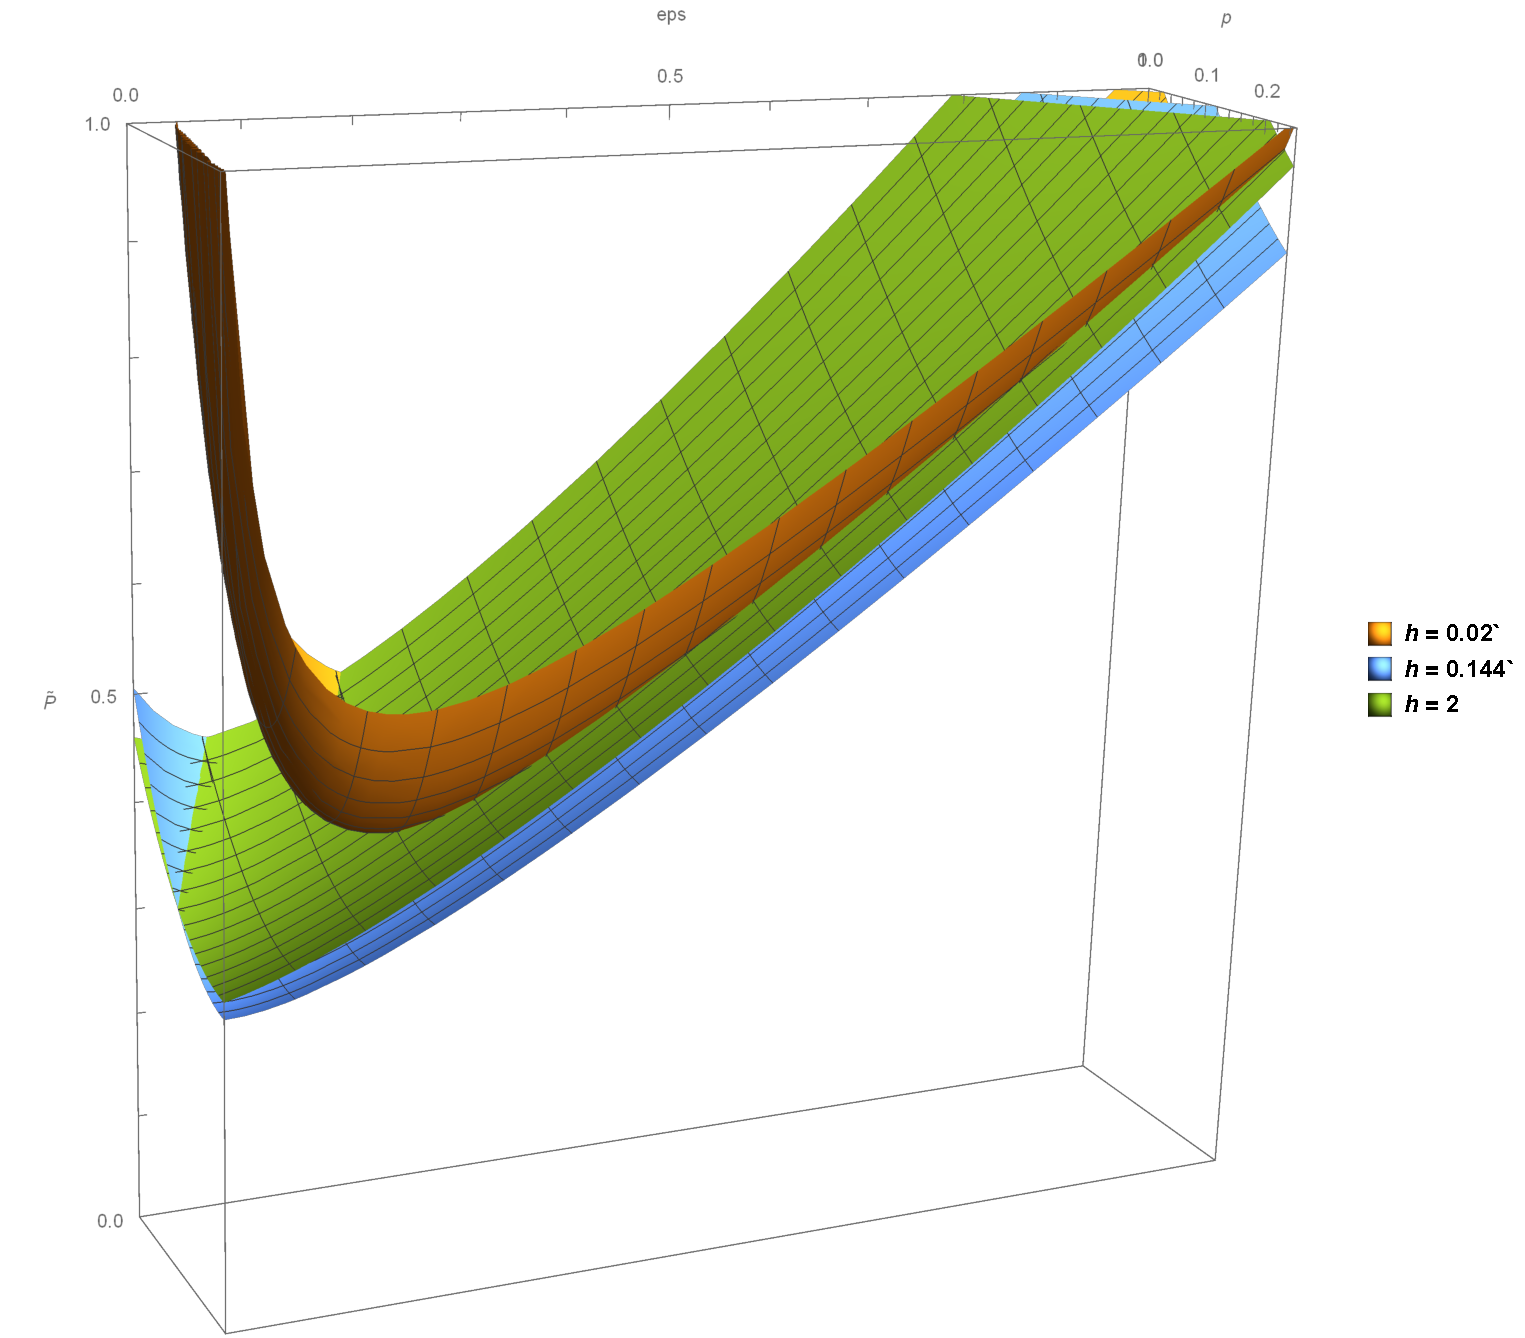
\includegraphics[width=0.9\textwidth]{Pepsandpone.pdf}
 \label{1b}\hfill}
%\subcaption{$h_1=0.144,h_2=0.6$}
 \caption{Global minima for fixed $\del=0.5$ and three heights $h=h_1$  over  $\eps\in[0,1]$ and $p=p_1\in[0,0.25]$.
   For $h=h_1=0.144$ the blue plot achieves the ``global'' minimum at $\eps=0$ and $p_1=0.25$. Note, that the brown curve
 not achiev its local minimum for same heights, since $\eps\sim0.15$.}\label{fig:globalnum_fixheight}
\end{figure}


\fi

\color{black}

%\section{Algorithms for deriving Möbius diagrams}
%
To obtain the ground terminal cells we need to derive for a given UAV deployment $\vQ=(\vP,\vH)$ its Möbius diagram. 
Since our performance function is a special case of a Möbius diagram, we might be simplify the algorithms for this
non-affine construction \cite{BWY07}.

Let us observe that for each $n\not=m$ we have by \lemref{lem:moebiusdia}
%
\begin{align}
  c_{nm}=c_{mn} \quad, \quad r_{nm}=r_{mn}
\end{align}
%
and by \eqref{eq:moebius}
%
\begin{align}
  V_{nm}=V_{mn}^c. 
\end{align}
%
Hence, we will reorder the $N$ coordinates $q_1,\dots,q_N$ in ascending order of their heights, i.e.,
%
\begin{align}
  \tQ=(\tq_1,\tq_2,\dots,\tq_N) \quad,\quad \tilde{h}_1\geq \tilde{h}_2\geq \dots\geq \tilde{h}_N.
\end{align}
%
This allows to derive two symmetric centroid and radii matrices
%
%\newcommand{\tilr}{\ensuremath{\tilde{r}}}
\begin{align}
  \tC=\begin{pmatrix}
    \tc_{11} & \tc_{12} & \dots & \tc_{1N}\\ 
    \tc_{21} & \tc_{22} & \dots & \tc_{2N}\\ 
    \vdots   &          & \ddots & \vdots\\
    \tc_{N1} & \tc_{N2} & \dots & \tc_{NN}\\ 
  \end{pmatrix}
  \quad,\quad
  \tR=\begin{pmatrix}
    \tilr_{11} & \tilr_{12} & \dots & \tilr_{1N}\\ 
    \tilr_{21} & \tilr_{22} & \dots & \tilr_{2N}\\ 
    \vdots   &          & \ddots & \vdots\\
    \tilr_{N1} & \tilr_{N2} & \dots & \tilr_{NN}\\ 
  \end{pmatrix}
\end{align}
%
Then $n$th row will generate the $n$th Möbius region by
%
\begin{align}
  \tV_n= \Big( \bigcap_{1\leq i< n}  B(\tc_{ni},\tilr_{ni})\Big) \cap \Big( \bigcap_{n<i\leq N}
  B(\tc_{ni},\tilr_{ni})^c\Big)
\end{align}
%
Obviously, if the centroids of two balls have distance larger then the sum of their radii, then the intersection will be
empty. We will therefore need to calculate  for $n<i<j\leq N$
%
\begin{align}
  d^{(n)}_{i,j}= |\tc_{ni}-\tc_{nj}|\quad,\quad \tilr^{(n)}_{i,j}=\tilr_{ni}+\tilr_{nj} 
\end{align}
%
Furthermore, if $\tilr_{ni}=\min\{\tilr_{ni},\tilr_{nj}\}\leq d^{(n)}_{i,j}$, then $C_{ni}$ is contained in $C_{nj}$ 

%\section{UAV as flying Base-Stations}
%
We will extend our UAV setup to a flying base-station scenario, where each UAV act as a relay between the base-station
and a ground terminal user, see for example \cite{AG18}.
We assume that the GTs are placed on $\Omega$ according to a time-invariant density function
$f:\mathbb{R}^2\to\mathbb{R}$, where $\int_{\Omega}f(\omega)d\omega=1$ \cite{GJ,Erdem1,ML,MLCS}. Further, the $N$ UAVs
are positioned at $(\vP,\vH)$ and will relay the communication from a base-station at $q^B=(p^B_x,p^B_y,h^B)$
as in \figref{fig:uavbasestation}. Thus, the total UAV
transmit power or average GT transmit power can be rewritten as
%
\begin{equation}
D\left(\bP,\bH\right)=\int_{\Omega}\min_{n}\left\{\beta\frac{\left(\|p_n-\omega\|^2+h^2_n\right)^{\frac{1+\alpha}{2}}}{h_n}
+ {\underbrace{\Norm{q_n-q^B}}_{=d_n^B}}^{{\alp}}\right\}f\left(\omega\right)d\omega,
\label{eq:Dbasestation}
\end{equation}
%
where we assume that the UAV has a directed perfectly aligned antenna to the base station, such that for $\tht=0$ by
\eqref{eq:Gdirected} it holds for the antenna relative radiation intensity $G_{BS}=1$. Hence, only the path loss exponent remains.
By setting the base-station at $q^B=(0,0,h^B)$ we get
\begin{align}
D\left(\bP,\bH\right)=\int_{\Omega}\min_{n}\left\{\beta\frac{\left(\|p_n-\omega\|^2+h^2_n\right)^{\frac{1+\alpha}{2}}}{h_n}
+ (\Norm{p_n}^2+(h_n-h^B)^2)^{\frac{\alp}{2}}\right\}f\left(\omega\right)d\omega.
\label{eq:Dbasestation2}
\end{align}

%
\begin{figure}
  \centering
  \def\svgwidth{.9\textwidth} \scriptsize{
    \input{UAVquacopter2_relay.pdf_tex}}
    \caption{UAV base-station deployment with directed antenna beam for $\alp=2$ and $N=2$ for a uniform GT distribution
    and perfect antenna alignment to the ground base-station at $q^B=(0,0,h^B)$.}
    \label{fig:uavbasestation}
\end{figure}



%\appendices
\appendix

\if0 % not relevant anymore, old Jun stuff
\junstart \section{Proof of Corollary \ref{corollary:continuity}}\label{proof:continuity} 

For convenience, we defined $\bar{\Vor}_n(p^*,
h^*)\triangleq\bigcup_{k=1}^{K_n}\bar{v}_{nk}$, be the $n$th normalized Voronoi region, where
$\bar{v}_{nk}\triangleq[a_{nk-1}-p^*_n,a_{nk}-p^*_n]$.
%Without loss of generality, we assume UAVs' ground projections are assigned in ascending order, i.e., $p_1 \le p_2 \le
%\cdots, \le p_N$.
In addition, the left and right Voronoi region of UAV $n$ is defined as $\bar{\Vor}^{L}_{n}(p^*, h^*) \triangleq
[s,p_n]\bigcap\bar{\Vor}_{n}(p^*, h^*)$ and $\bar{\Vor}^{R}_{n}(p^*, h^*) \triangleq [p_n, t]\bigcap\bar{\Vor}_{n}(p^*,
h^*)$, respectively.  Let $\mu^L_n\triangleq\mu\left(\bar{\Vor}^{L}_{n}(p^*, h^*)\right)$ and
$\mu^R_n\triangleq\mu\left(\bar{\Vor}^{R}_{n}(p^*, h^*)\right)$ be the Lebesgue measure of the left and right Voronoi
regions.

We assume that UAV $m$'s Voronoi region is discontinuous, i.e., $K_m\ge2$.  Let $(\widetilde{p},h^*)$ be an alternative
deployment where $\widetilde{p}_n=b_{n-1}+\mu^L_{n}$ is a point in $\widetilde{\Vor}_n$ and
$\widetilde{\Vor}_{n}=[b_{n-1}, b_n]$ is a continuous region where
$b_n=s+\sum_{i=1}^{n}\mu\left({\Vor}_{n}(p^*,h^*)\right)$.  By straightforward calculation, we have
$\mu(\widetilde{V}_{n})=b_n-b_{n-1}=\mu({V}_{n}(p^*,h^*))=\mu^L_n+\mu^R_n$.  The difference of the distortion of the two
deployment is
%
\begin{equation}
\begin{aligned}
    &\abPo\left(\bP^*,\bH^*\right) - \abPo\left(\widetilde{\bP},\bH^*\right)\\
    \overset{(a)}{=}&\sum_{n=1}^{N}\left[\int_{\Vor_n\left(p^*, h^*\right)}  \frac{ \left(\Norm{p^*_n- \ome}^2 \!+\!(h^*_n)^2\right)^{\gam}}{h^*_n} \df(\ome)d\ome-\int_{\widetilde{\Vor}_{n}} \frac{ \left(\Norm{\widetilde{p}_n- \ome}^2 \!+\!(h^*_n)^2\right)^{\gam}}{h^*_n} \df(\ome)d\ome\right]\\
    \overset{(b)}{=}&\frac{1}{t\!-\!s}\sum_{n=1}^{N}\left[\int_{\bar{\Vor}_n\left(p^*, h^*\right)}  \frac{ \left(u^2 \!+\!(h^*_n)^2\right)^{\gam}}{h^*_n} du-\int_{-\mu^L_n}^{\mu^R_n} \frac{ \left(\nu^2 \!+\!(h^*_n)^2\right)^{\gam}}{h^*_n} d\nu\right]\\
    \overset{(c)}{=}&\frac{1}{t\!-\!s}\sum_{n=1}^{N}\left[\int_{\bar{\Vor}^L_n\left(p^*, h^*\right)}  \frac{ \left(\ome^2 \!+\!(h^*_n)^2\right)^{\gam}}{h^*_n} d\ome-\int_{-\mu^L_n}^{0} \frac{ \left(\ome^2 \!+\!(h^*_n)^2\right)^{\gam}}{h^*_n} d\ome\right]\\
    &+\frac{1}{t\!-\!s}\sum_{n=1}^{N}\left[\int_{\bar{\Vor}^R_n\left(p^*, h^*\right)}  \frac{ \left(\ome^2 \!+\!(h^*_n)^2\right)^{\gam}}{h^*_n} d\ome-\int_{0}^{\mu^R_n} \frac{ \left(\ome^2 \!+\!(h^*_n)^2\right)^{\gam}}{h^*_n} d\ome\right]\\
    \overset{(d)}{=}&\frac{1}{t\!-\!s}\sum_{n=1}^{N}\left[\int_{\bar{\Vor}^L_n\left(p^*, h^*\right)\setminus[-\mu^L_n, 0]}  \frac{ \left(\ome^2 \!+\!(h^*_n)^2\right)^{\gam}}{h^*_n} d\ome-\int_{[ -\mu^R_n,0]\setminus\bar{\Vor}^R_n\left(p^*, h^*\right)} \frac{ \left(\ome^2 \!+\!(h^*_n)^2\right)^{\gam}}{h^*_n} d\ome\right]\\
    &+\frac{1}{t\!-\!s}\sum_{n=1}^{N}\left[\int_{\bar{\Vor}^R_n\left(p^*, h^*\right)\setminus[0, \mu^R_n]}  \frac{ \left(\ome^2 \!+\!(h^*_n)^2\right)^{\gam}}{h^*_n} d\ome-\int_{[0, \mu^R_n]\setminus\bar{\Vor}^R_n\left(p^*, h^*\right)} \frac{ \left(\ome^2 \!+\!(h^*_n)^2\right)^{\gam}}{h^*_n} d\ome\right]\\
    \overset{(e)}{\le}&0,
\end{aligned}
\end{equation}
where (a) follows from the definition of $\abPo\left(\bP,\bH\right)$, (b) follows from $u=\ome-p^*_n$ and $\nu=\ome-\widetilde{p}_n+p^*_n$, (e) follows from (i) $\ome^2\ge\mu^L_n$ when $\ome\in\bar{\Vor}^L_n\left(p^*, h^*\right)\setminus[-\mu^L_n, 0]$, (ii)  $\ome^2\le\mu^L_n$ when $\ome\in[-\mu^L_n, 0]\setminus\bar{\Vor}^L_n\left(p^*, h^*\right)$, (iii) $\ome^2\ge\mu^R_n$ when $\ome\in\bar{\Vor}^R_n\left(p^*, h^*\right)\setminus[0, \mu^R_n]$, and (iv) $\ome^2\le\mu^R_n$ when $\ome\in[0, \mu^R_n]\setminus\bar{\Vor}^R_n\left(p^*, h^*\right)$.
Note that (e) is an equality if and only if $\bar{\Vor}_n\left(p^*, h^*\right)=[-\mu^L_n,\mu^R_n]$ is a continuous region.
Since $\Vor_m\left(p^*, h^*\right)$ is discontinuous, $\bar{\Vor}_m\left(p^*, h^*\right)$ cannot be a continuous region, indicating the equality is not achievable.
Therefore, $(\widetilde{p}, h^*)$ is a better deployment than $(p^*, h^*)$, which contradicts our consumption.
Consequently, all optimal regions are continuous.

\section{Proof of Corollary \ref{corollary:linearity}}\label{proof:linearity}
The distortion for one UAV over the uniformly distributed one-dimensional space $[s,t]$ is
\begin{align}
    \abPo(p_1,h_1)= \int_{s}^{t} \frac{\left(\Norm{p_1-\ome}^2 + h^2_1\right)^\gam}{h_1} \df(\ome)d\ome
\end{align}
We get by substituting $\tome=p_1-\ome$
\begin{align}
    \abPo(p_1,h_1)= \frac{1}{\mu(\Omega)}\int_{p_1-t}^{p_1-s} \frac{\left(\tome^2 + h^2_1\right)^{\gam}}{h_1} d\tome
\end{align}
A critical point $q^*_1=\left(p^*_1, h^*_1\right)$ is only attained if all its first-order partial derivatives are vanishing, i.e.,  for  $n=1,2,\dots,N$, 
%
\begin{align}
  \frac{\partial \abPo(p_1,h_1)}{\partial p_1}\Big|_{(p^*_1,h^*_1)}\!\!= \frac{1}{\mu(\Omega)h_1}\left[\left(\left(p_1\!-\!s\right)^2\!+\!h_1^2\right)^{\gam\!-\!1}d\ome\!-\!\left(\left(p_1\!-\!t\right)^2!+\!h_1^2\right)^{\gam\!-\!1}d\ome\right] \Big|_{(p^*_1,h^*_1)} = 0 \label{dp}\\
  \frac{\partial\abPo(p_1,h_1)}{\partial h_1}\Big|_{(p^*_1,h^*_1)} = \frac{1}{\mu(\Omega)h_1^2}\int_{p_1-t}^{p_1-s}\!\!\left(\ome^2 +h_1^2\right)^{\gam\!-\!1}\!\cdot  \big(\left(2\gamma\!-\!1\right)h_1^2\!-\!\ome^2 \big)
  d \ome\Big|_{(p^*_1,h^*_1)} = 0
\label{dh}
\end{align}
Solving (\ref{dp}), we get the optimal projection
\begin{align}
    p^*_1 = \frac{s+t}{2}\label{eq:centroidProjection}
\end{align}
Then, the second-order derivative over $h_1$ at $p_1=p^*_1$ is
\begin{align}
    \frac{\partial^2 \abPo(p^*_1,h_1)}{\partial h^2_1} = \frac{1}{\mu(\Omega)}\int_{-\mu(\Omega)/2}^{\mu(\Omega)}\frac{2h(\ome^2+h^2)^{\gamma-2}\left[\frac{3}{4}\gamma^2+\left(\left(\frac{2-\gamma}{2}\right)h^2+\ome^2\right)^2\right]}{h^4}d\ome > 0
    \label{d2p}
\end{align}
Thus, $\frac{\partial \abPo(p^*_1,h_1)}{\partial h_1}$ has at most one real root, indicating that ${\abPo}(p^*_1,h_1)$ has at most one minimum. 
On the other hand, since ${\abPo}(p^*_1,h_1)>0$, $\lim\limits_{h_1\to0}{\abPo}(p^*_1,h_1)=+\infty$ and  $\lim\limits_{h_1\to+\infty}{\abPo}(p^*_1,h_1)=+\infty$ when $\gamma>=1$, we conclude that ${\abPo}(p^*_1,h_1)$ has at least one minimum.
As a result, ${\abPo}(\bP^*,\bH)$ has exact one minimum.

In what follows, we prove that the optimal flight height, $h^*_1$, is proportional to $\mu(\Omega)$.
Let $g(\gamma)\triangleq\arg\min\limits_{h}\int_{-1/2}^{1/2} \frac{\left(\ome^2 + h^2\right)^{\gam}}{h} d\ome$ be the optimal flight height over $[-\frac{1}{2}, \frac{1}{2}]$.
Then, we have 
\begin{align}
\frac{\partial\abPo(p_1,h_1)}{\partial h_1}\Big|_{(0,g(\gamma))}\!\!=\! \frac{1}{g^2(\gamma)}\!\int_{-1/2}^{1/2}\!\!\left(\ome^2\! +\!g^2(\gamma)\right)\!\!^{\gam\!-\!1}\!\!\cdot \big(\!\left(2\gamma\!-\!1\right)g^2(\gamma)\!-\!\ome^2 \big)
  d \ome \!=\!0
  \label{pphh}
\end{align}  
For an arbitrary target region $\Omega=[s,t]$, the first-order derivative over $h_1$ at $(p^*_1, g(\gamma)\mu(\Omega)$ is
\begin{align}
\frac{\partial\!\abPo(p_1,\!h_1)}{\partial h_1}
&\overset{(a)}{=}\frac{1}{\mu(\Omega)\left(g(\gamma)\mu(\Omega)\right)^2}\!\int_{-\frac{\mu(\Omega)}{2}}^{\frac{\mu(\Omega)}{2}}\!\!\left(\ome^2\!\!+\!\left(g(\gamma)\mu(\Omega)\right)^2\right)\!\!^{\gam\!-\!1}\!\!\cdot\!  \big(\!\left(2\gamma\!\!-\!\!1\right)\left(g(\gamma)\mu(\Omega)\right)^2\!\!-\!\!\ome^2 \big)
  d \ome\\
&\overset{(b)}{=}\frac{\left(\mu(\Omega)\right)^{2\gamma-2}}{g^2(\gamma)}\int_{-1/2}^{1/2}\!\!\left(\ome^2\! +\!g^2(\gamma)\right)\!\!^{\gam\!-\!1}\!\!\cdot \big(\!\left(2\gamma\!-\!1\right)g^2(\gamma)\!-\!\ome^2 \big)
  d \ome \overset{(c)}{=}0
\end{align}
where (a) follows from $p_1=p^*_1$ and $h_1=g(\gamma)\mu(\Omega)$, (b) follows from $\tome=\frac{1}{\mu(\Omega)}\ome$, and (c) follows from (\ref{pphh}).
Therefore, single UAV's optimal flight height $h^*_1$ is proportional to the Lebesgue measure $\mu(\Omega)$, i.e., $h^*_1=g(\gamma)\mu(\Omega)$.

\section{Proof of Theorem \ref{theorem:commonHeight}}\label{uniformQuantizer}
%Now we have enough materials to prove Theorem \ref{theorem:commonHeight}.
Let $(p^*,h^*)$ be the optimal UAV deployment over the one-dimension ground $\Omega=[s,t]$ with uniform density function $\lambda(\ome)=\frac{1}{\mu(\Omega)}$, where $\mu(\Omega)=t-s$ is the Lebesgue measure (volume).

Since the distortion function 
\begin{align}
  f(\ome,p,h)= \left(h_n^{-\frac{1}{\gamma}}\Norm{p-\ome}^2 + h_n^{2-\frac{1}{\gamma}}\right)^{\gamma}
\end{align}  
is a polynomial in $\ome$ of degree less than $2\gamma$ for each fixed $\bQ=(p,h)$, the average distortion function is continuous
differentiable, and we obtain by \cite[Thm.1]{WJ18} for the partial derivatives 
%
\begin{align}
  \frac{\partial \Pbar(q)}{\partial q_{n,i}} = \int_{\Vor_n(q)} \frac{\partial f(\ome,q)}{\partial q_{n,i}}
  \df(\ome)d\ome\quad,\quad i\in\{1,2,3\},n\in\{1,2,\dots,N\}.
\end{align}
%
Hence, a critical point is only attained if all its partial derivatives are vanishing, i.e.,  for  $n=1,2,\dots,N$ 
%
\begin{align}
 0\overset{!}{=} \nabla_n \Pbar(p,h) &= \begin{pmatrix} 
   \int_{\Vor_n} 2h_n^{-1} \gam (p_{n}-\ome)  \left(\Norm{p_n-\ome}^2 +h_n^2\right)^{\gam-1} 
    \df(\ome)d \ome\\
    \int_{\Vor_n} \left[-h_n^{-2}(\Norm{p_n-\ome}^2 + h_n^2)^{\gam} + 2\gam 
    (\Norm{p_n-\ome}^2 +h_n^2)^{\gam-1}\right]
    \df(\ome)d \ome
  \end{pmatrix} \in\R^3\notag\\
\LRA 0&= \begin{pmatrix}
  \int_{\Vor_n} (p_{n}-\ome) (\Norm{p_n-\ome}^2 +h_n^2)^{\gam-1} \df(\ome)d \ome\\
  \int_{\Vor_n} (\Norm{p_n-\ome}^2 +h_n^2)^{\gam-1}\cdot \big(\Norm{p_n-\ome}^2+h_n^2 - 2\gam h_n^2 \big)
  \df(\ome)d \ome
  \end{pmatrix}\label{eq:gradient}
\end{align}
%
By Corollary \ref{corollary:continuity}, the optimal Voronoi regions are continuous intervals. 
Without loss of generality, we assume that the Voronoi regions are assigned in ascending order, i.e., 
\begin{align}
\Vor(p^*, h^*)=[b^*_{n-1}, b^*_n], \forall n\in\{1,\dots,N\},
\label{eq:1DoptV}
\end{align}
where $b^*_0\le b^*_1\le\dots\le b^*_N$ are the optimal Voronoi region boundaries. In particular, we have $b^*_0=s$ and $b^*_N=t$.
By Lemma \ref{lemma:allActive}, all UAVs has positive volume indicating $b_n > b_{n-1}, \forall n\in\{0,1,\dots,N\}$.
In other words, the boundaries are strictly increasing, i.e., $b^*_0< b^*_1<\dots< b^*_N$.
Let $\mu_n=b^*_n-b^*_{n-1}, \forall n\in\{1,\dots,N\}$ be the volume of partition $\Vor_n(p^*, h^*)$, where $\sum_{n=1}^{N}\mu_n=\mu(\Omega)$.
By Corollary \ref{corollary:linearity}, UAV $n$'s optimal deployment is $p^*_n=\frac{b^*_{n-1}+b^*_{n}}{2}$ and $h^*_n=g(\gamma)\mu_n$.
Accordingly, the minimum distortion can be rewritten as
\begin{align}
    &\abPo(\bP^*,\bH^*)=\sum_{n=1}^{N}\int_{b^*_{n-1}}^{b^*_{n}}\frac{\left(\|p_n-\ome\|^2+h^*_n\right)^{\gamma}}{h^*_n}\df(\ome) d\ome\\
    \overset{(a)}{=}&\sum_{n=1}^{N}\int_{-1/2}^{1/2} \frac{\left(\mu^2_n\ome^2_n+(h^*_n)^2\right)^{\gamma}}{h^*_n} \frac{\mu_n}{\mu(\Omega)}d\ome_n\\
    \overset{(b)}{=}&\sum_{n=1}^{N}\int_{-1/2}^{1/2}\frac{\left(\mu^2_n\ome^2_n+g^2(\gamma)\mu^2_n\right)^{\gamma}}{g(\gamma)\mu_n} \frac{\mu_n}{\mu(\Omega)}d\ome_n\\
    \overset{(c)}{=}&\int_{-1/2}^{1/2}\frac{\left(\ome^2_n+g^2(\gamma)\right)^{\gamma}}{g(\gamma)} \frac{1}{\mu(\Omega)}d\ome\sum_{n=1}^{N}\mu^{2\gamma}_n\\
    \overset{(d)}{\ge}&\frac{\left(\mu(\Omega)\right)^{2\gamma-1}}{N^{2\gamma-1}}\int_{-1/2}^{1/2}\frac{\left(\ome^2+g^2(\gamma)\right)^{\gamma}}{g(\gamma)} d\ome
  \end{align}
where (a) follows from $\ome_n=\frac{p_n-\ome}{\mu_n}$, (b) follows from $h^*_n=g(\gamma)\mu_n$, and (d) is an equality if and only if $\mu_n=\frac{\mu(\Omega)}{N}$.
Therefore, the optimal flight heights are $h^*_n=g(\gamma)\mu_n=\frac{g(\gamma)\mu(\Omega)}{N}, \forall n\in\{1,\dots,N\}$, the optimal partition boundaries are $b^*_n=s+\frac{t-s}{N}n, \forall n\in\{1,\dots,N\}$, the optimal projections are $p^*_n=\frac{b^*_{n-1}+b^*_{n}}{2}=s+\frac{(n-1/2)(t-s)}{N}, \forall n\in\{1,\dots,N\}$, and the minimum distortion is $\frac{\left(\mu(\Omega)\right)^{2\gamma-1}}{N^{2\gamma-1}}\int_{-1/2}^{1/2}\frac{\left(\ome^2+g^2(\gamma)\right)^{\gamma}}{g(\gamma)} d\ome$.
%In other words, UAV $n$'s optimal ground projection should be at the centroid of its Vonoroi region $\Vor_n(p^*_n, h^*_n)$.
%Substituting (\ref{eq:centroidProjection}) and (\ref{eq:1DoptV}) to (\ref{eq:gradient}), we have
\fi
\junend
\philippstart
%% Detailed proof of uniform scalar quantizer (bounded)
\section{Proof of Uniform Scalar Quantizer}\label{app:UniformScalarQuantizer}
\begin{proof}[Proof of \lemref{lem:UniformScalarQuantizer}]
  By the \emph{conservation law of
  mass} \cite[Thm.2.2]{CMB05}, the partial derivatives of $H_V(\vx)$ after $x_n$ are given by
  %
  \begin{align}
   \frac{\partial H_V(\vx)}{\partial x_n} &= \int_{\Vor_n(\vx)} \frac{ \partial (x_n-\ome)^2}{\partial x_n} d\ome 
    &\RA\quad   0\overset{!}{=}  \int_{\Vor_n(\vx^*)}(x_n^*-\ome) d\ome \LRA x_n^*=\frac{\int_{\Vor_n(\vx^*)}
  \ome d\ome}{\int_{\Vor_n(\vx^*)} d\ome}
    \label{eq:nint}
  \end{align}
  %
  which is the centroid of the optimal Voronoi region $\Vor_n(\vx^*)$. 
  %
  Since the Voronoi region depend on all $x_n$ we need the explicit parameterization of the regions.  W.l.o.g. we can
  label the $N$ quantizer points such that their ground positions are in increasing order, i.e., $0\leq x_1 < x_2 < \dots < x_N\leq
  A$, where we assume that all $N$ points are different and contained in the target region $\Ome=[0,A]$,
  otherwise not all points would be active and the number of effective points would be less than $N$. We will show later,
  that inactive points will increase the objective function and therefore not yield the global minimum. Each Euclidean
  Voronoi region is by definition  the intersection of $N-1$ dominance regions $\Vor_{nm}(\vx)=[0,(x_m+x_n)/2]$ for
  $n<m$ and $[(x_n+x_m)/2,A]$ for $n>m$ given by
  %
   \begin{align}
       \Vor_n(\vx) &= \bigcap_m \Vor_{nm}(\vx)=\bigcap_{n<m} [0,\frac{x_m\!+\!x_n}{2}] \bigcap_{n>m} [\frac{x_n\!+\!x_m}{2},A] \\
       &=[b_{n-1},b_n]
       =\begin{cases} 
       [0,\frac{x_2+x_1}{2}] &, n=1\\
       [\frac{x_{N}+x_{N-1}}{2},A] &, n=N\\
       [\frac{x_{n}+x_{n-1}}{2},\frac{x_{n+1}+x_n}{2}] &,\text{else}
       \end{cases}\label{eq:Vorn}
  \end{align}
  %
  The integral of the centroid \eqref{eq:nint} can then be calculated  as
  %
  \begin{align}
      x_n^* &= \frac{ \frac{1}{2} \ome^2 \Big|_{a_n^*}^{b_n^*}}{ b_n^*-a_n^*}
      = \frac{1}{2} \frac{(b_n^*)^2-(a_n^*)^2}{b_n^*-a_n^*} = \frac{b_n^*+a_n^*}{2} \label{eq:xniterative}.
  \end{align}
  %
  For $1<n<N$ we get
  %
  \begin{align}
    x_n^*=\frac{x_{n+1}^*+ 2x_n^*+x_{n-1}^*}{4} = \frac{x_{n+1}^*+x_{n-1}^*}{4} +\frac{x_n^*}{2}\quad\RA \quad x_n^*
    =\frac{x_{n+1}^*+x_{n-1}^*}{2}\label{eq:midpoints}.
  \end{align}
  %
  For $n=1$ and $n=N$ we get 
  %
  \begin{align}
      x_1^*=\frac{1}{3}x_2^* \quad,\quad x_N^* = \frac{1}{3}(2A+x^*_{N-1})\label{eq:firstlast}.
  \end{align}
  %
  The two equations contain $4$ unknowns and are therefore under-determined. To resolve the positions, we need to
  extract from \eqref{eq:midpoints} two more equations in the same $4$ unknowns $x_1,x_2,x_N,x_{N-1}$
  (Let us omit the star-index for now).
  We prove by induction that it holds for each $N-1\geq m\geq 2$ 
  %
  \begin{align}
    P(m) :\LRA x_1 = m x_{m} -(m-1) x_{m+1} \label{eq:Pm}.
  \end{align}
  %
  Let us resolve \eqref{eq:midpoints} to 
  %
  \begin{align}
    x_{n-1}=2x_n-x_{n+1} \quad,\quad N-1\geq n\geq 2\label{eq:xn1}
  \end{align}
  %
  then for $m=n=2$ this proofs the induction start $P(2)$. Let us assume $P(m)$ is true, than we get with
  $m=n-1\geq 2$ in \eqref{eq:xn1}  
  %
  \begin{align}
    x_1=mx_m - (m-1)x_{m+1} = m(2x_{m+1} -x_{m+2})-(m-1)x_{m+1}= (m+1)x_{m+1}  -mx_{m+2}\notag
  \end{align}
  %
  which proofs  $P(m+1)$ and therefore the assumption $P(m)$ for all $N-1\geq m\geq 2$.
  %
  Similar we can show for $N-1\geq m\geq 2$ the assertion 
  %
  \begin{align}
    \tP(m):\LRA x_N= mx_{N-(m-1)} - (m-1)x_{N-m}.
  \end{align}
  %
  Resolving \eqref{eq:xn1} to $x_{n+1}=2x_n-x_{n-1}$ yields for $m=2$ and $n=N-m+1$ the
  induction start $\tP(2)$ and with $\tP(m)$ and $n=N-m$ this shows $\tP(m+1)$.  
  Then from \eqref{eq:firstlast}, $P(N-1)$, and $\tP(N-1)$ we get the two equations
  %
  \begin{align}
    x_1 &= (N-1)(3x_{N}-2A)-(N-2)x_{N} = (2N-1)x_{N} -2(N-1)A\\
    x_N &= (N-1)x_{2} -(N-2)x_1=(N-1)3x_1-(N-2)x_1=(2N-1)x_1\label{eq:xN}
  \end{align}
  %
  which yields to
  %
  \begin{align}
    x_1= (2N-1)(2N-1)x_1-2(N-1)A \LRA A = \frac{4N^2-4N+1-1}{2(N-1)} x_1 \LRA x_1= \frac{A}{2N}.\label{eq:x1A}
  \end{align}
  %
  Inserting in \eqref{eq:xN} gives
  %
  \begin{align}
    x_N= \frac{(2N-1)A}{2N}.\label{eq:xNA}
  \end{align}
  %
  Together with \eqref{eq:xn1} this shows $x_n=(2n-1)A/(2N)$ for $n=1,2,\dots,N$ and $N=1,2,3$.
  For $N\geq 4$ we need to derive the pairwise ground distances, given for $N-1\geq m\geq 3$ by
  %
  \begin{align}
    \Del_m &= x_m-x_{m-1}\overset{P(m-1)}{=}x_m -\frac{x_1+(m-2)x_m}{m-1} = \frac{x_m-x_1}{m-1}\\
    \Del_m &= x_m-x_{m-1}\overset{\tP(N-m+1)}{=} x_m + \frac{x_N -(N-m+1)x_m}{N-m} = \frac{x_N-x_m}{N-m}  
  \end{align}
  %
  Eliminating $x_m$ yields to 
  %
  \begin{align}
    (m-1)\Del_m + x_1 = x_N-\Del_m(N-m) \LRA \Del_m= \frac{x_N-x_1}{N-1}
  \end{align}
  %
  Finally, inserting \eqref{eq:xNA} and \eqref{eq:x1A} yields to
  %
  \begin{align}
    \Del_m=\Del=\frac{(2N-1)A-A}{2N(N-1)}= \frac{A}{N}\label{eq:Del}
  \end{align}
  %
  and since $x_2-x_1= A/N=x_N-x_{N-1}$ by \eqref{eq:firstlast} and \eqref{eq:xN} resp. \eqref{eq:xNA}  \eqref{eq:Del}
  holds for $2\leq m\leq N$.  Hence, we get for $n=1,2,\dots,N$ and any $N\geq 1$
  %
  \begin{align}
      x_n^* =x_1^*+ (n-1) \Del=\frac{(2n-1)A}{2N}\label{eq:quantizern}.
  \end{align}
  %
  To derive the optimal height we need to calculate $H_V(\vx^*)$.  
  Calculating explicitly the integrals we get for the Euclidean distortion 
  %
  \begin{align}
   A H_V(\vx^{*}):= (\frac{1}{3} \Big((\ome-x_1^*)^3\Big|_{0}^{b_1}+ (\ome-x_N^*)^3\Big|_{b_{N-1}}^A \Big)
    + \sum_{n=2}^{N-1} \frac{1}{3}(\ome-x_n^{*})^3 \Big|_{b_{n-1}}^{b_n}
  \intertext{with the bisectors given by \eqref{eq:Vorn} and \eqref{eq:quantizern}}
    b_{n-1}=\frac{x^*_n+x^*_{n-1}}{2}= \frac{(2n-1 +(2(n-1)-1)))A}{2\cdot 2N}= \frac{(n-1)A}{N} \quad\text{and}\quad b_0=0,
    b_N=A.
  \end{align}
  %
  The difference is then given by
  %
  \begin{align}
     \frac{1}{3}\sum_n \left( \Big(\frac{(2n - (2n-1))A }{2N}\Big)^3-\Big(\frac{(2n-2-(2n-1))A}{2N}\Big)^3\right)
     = \sum_n \frac{2 A^3}{3 \cdot 8 N^3} = (N-2)\frac{A^3}{12 N^3} \notag
  \end{align}
  %
  which yields with the first and last cell
  %
  \begin{align}
    \frac{1}{3}\left(\Big( \frac{2A\!-\!A}{2N}\Big)^3- \frac{-A^3}{(2N)^3} +
    \Big(\frac{2N A- (2N\!-\!1)A}{2N}\Big)^3 - \Big(\frac{2(N\!-\!1)A-(2N\!-\!1)A}{2N}\Big)^3\right)
    = \frac{4}{3} \Big(\frac{A}{2N}\Big)^3\notag
  \end{align}
  %
  to
  %
  \begin{align}
     H_V(\vx^{*})= \frac{1}{A} \left( (N-2) \frac{A^3}{12 N^3} + 2 \frac{A^3}{12 N^3}\right)= \frac{A^2}{12N^2}.
  \end{align}
  %
  Now we see, that if there are inactive quantization points, $N$ would decrease and the power consumption increase. Therefore, inactive
  point configurations can be seen as local minima and the all active case as the global minima.  
\end{proof}

\philippend
%\input{derivativeminmum}
%\input{generalizedVoronoi}
\printbibliography
\end{document}


